\chapter{Results}
This chapter aims to present the results to the reader.
As indicated in the methodology, we tested four mechanisms (three variants of kd-Laplace and Piecewise) for their utility and privacy.
\begin{enumerate}
      \item Cluster utility: Visualise the utility of kD-Laplace and Piecewise for 2/3/n-dimensional data.
            The results are displayed using a line diagram, using \gls{ami} and \gls{sc}.
      \item Mechanism utility: Visualise the utility of kD-Laplace and Piecewise using a heatmap plot.
            The results for each dimension and privacy budget are provided for only the \gls{ami} score.
      \item Mechanism privacy: Visualise the privacy of kD-Laplace and Piecewise using a heatmap plot.
            The results for each dimension and privacy budget are provided for only the adversary advantage and privacy distance.
      \item Mechanism comparison: Visualise the comparison between the variants of kD-Laplace and Piecewise.
            The results for each mechanism \& variant are provided using a bar-plot for the \gls{ami} score (utility) and the adversary advantage (privacy).
\end{enumerate}
All results are reported for each dataset (See methodology: \ref{datasets-section}) separately.
\section{Cluster utility}
The results below display the difference in external and internal utility for the three cluster algorithms using the kd-Laplace and Piecewise mechanisms.
The x-axis shows the privacy budget, and the y-axis shows the \gls{ami}.
Please refer to the plots in the appendix for the same scores for kD-Laplace variants (See \ref{appendix:results-mechanism-utility}).
\newpage
\subsection{2-dimensional data}
\begin{figure}[H]
      \centering
      \begin{subfigure}{0.3\textwidth}
            \includegraphics[width=\textwidth]{Results/kd-laplace/kd-Laplace/seeds-dataset/legend_2.png}
      \end{subfigure}
      \begin{subfigure}{1\textwidth}
            \centering
            \caption{\textbf{AMI (top) and SC (bottom) for the kD-Laplace mechanism for the 2-dimensional data seeds-dataset}}
            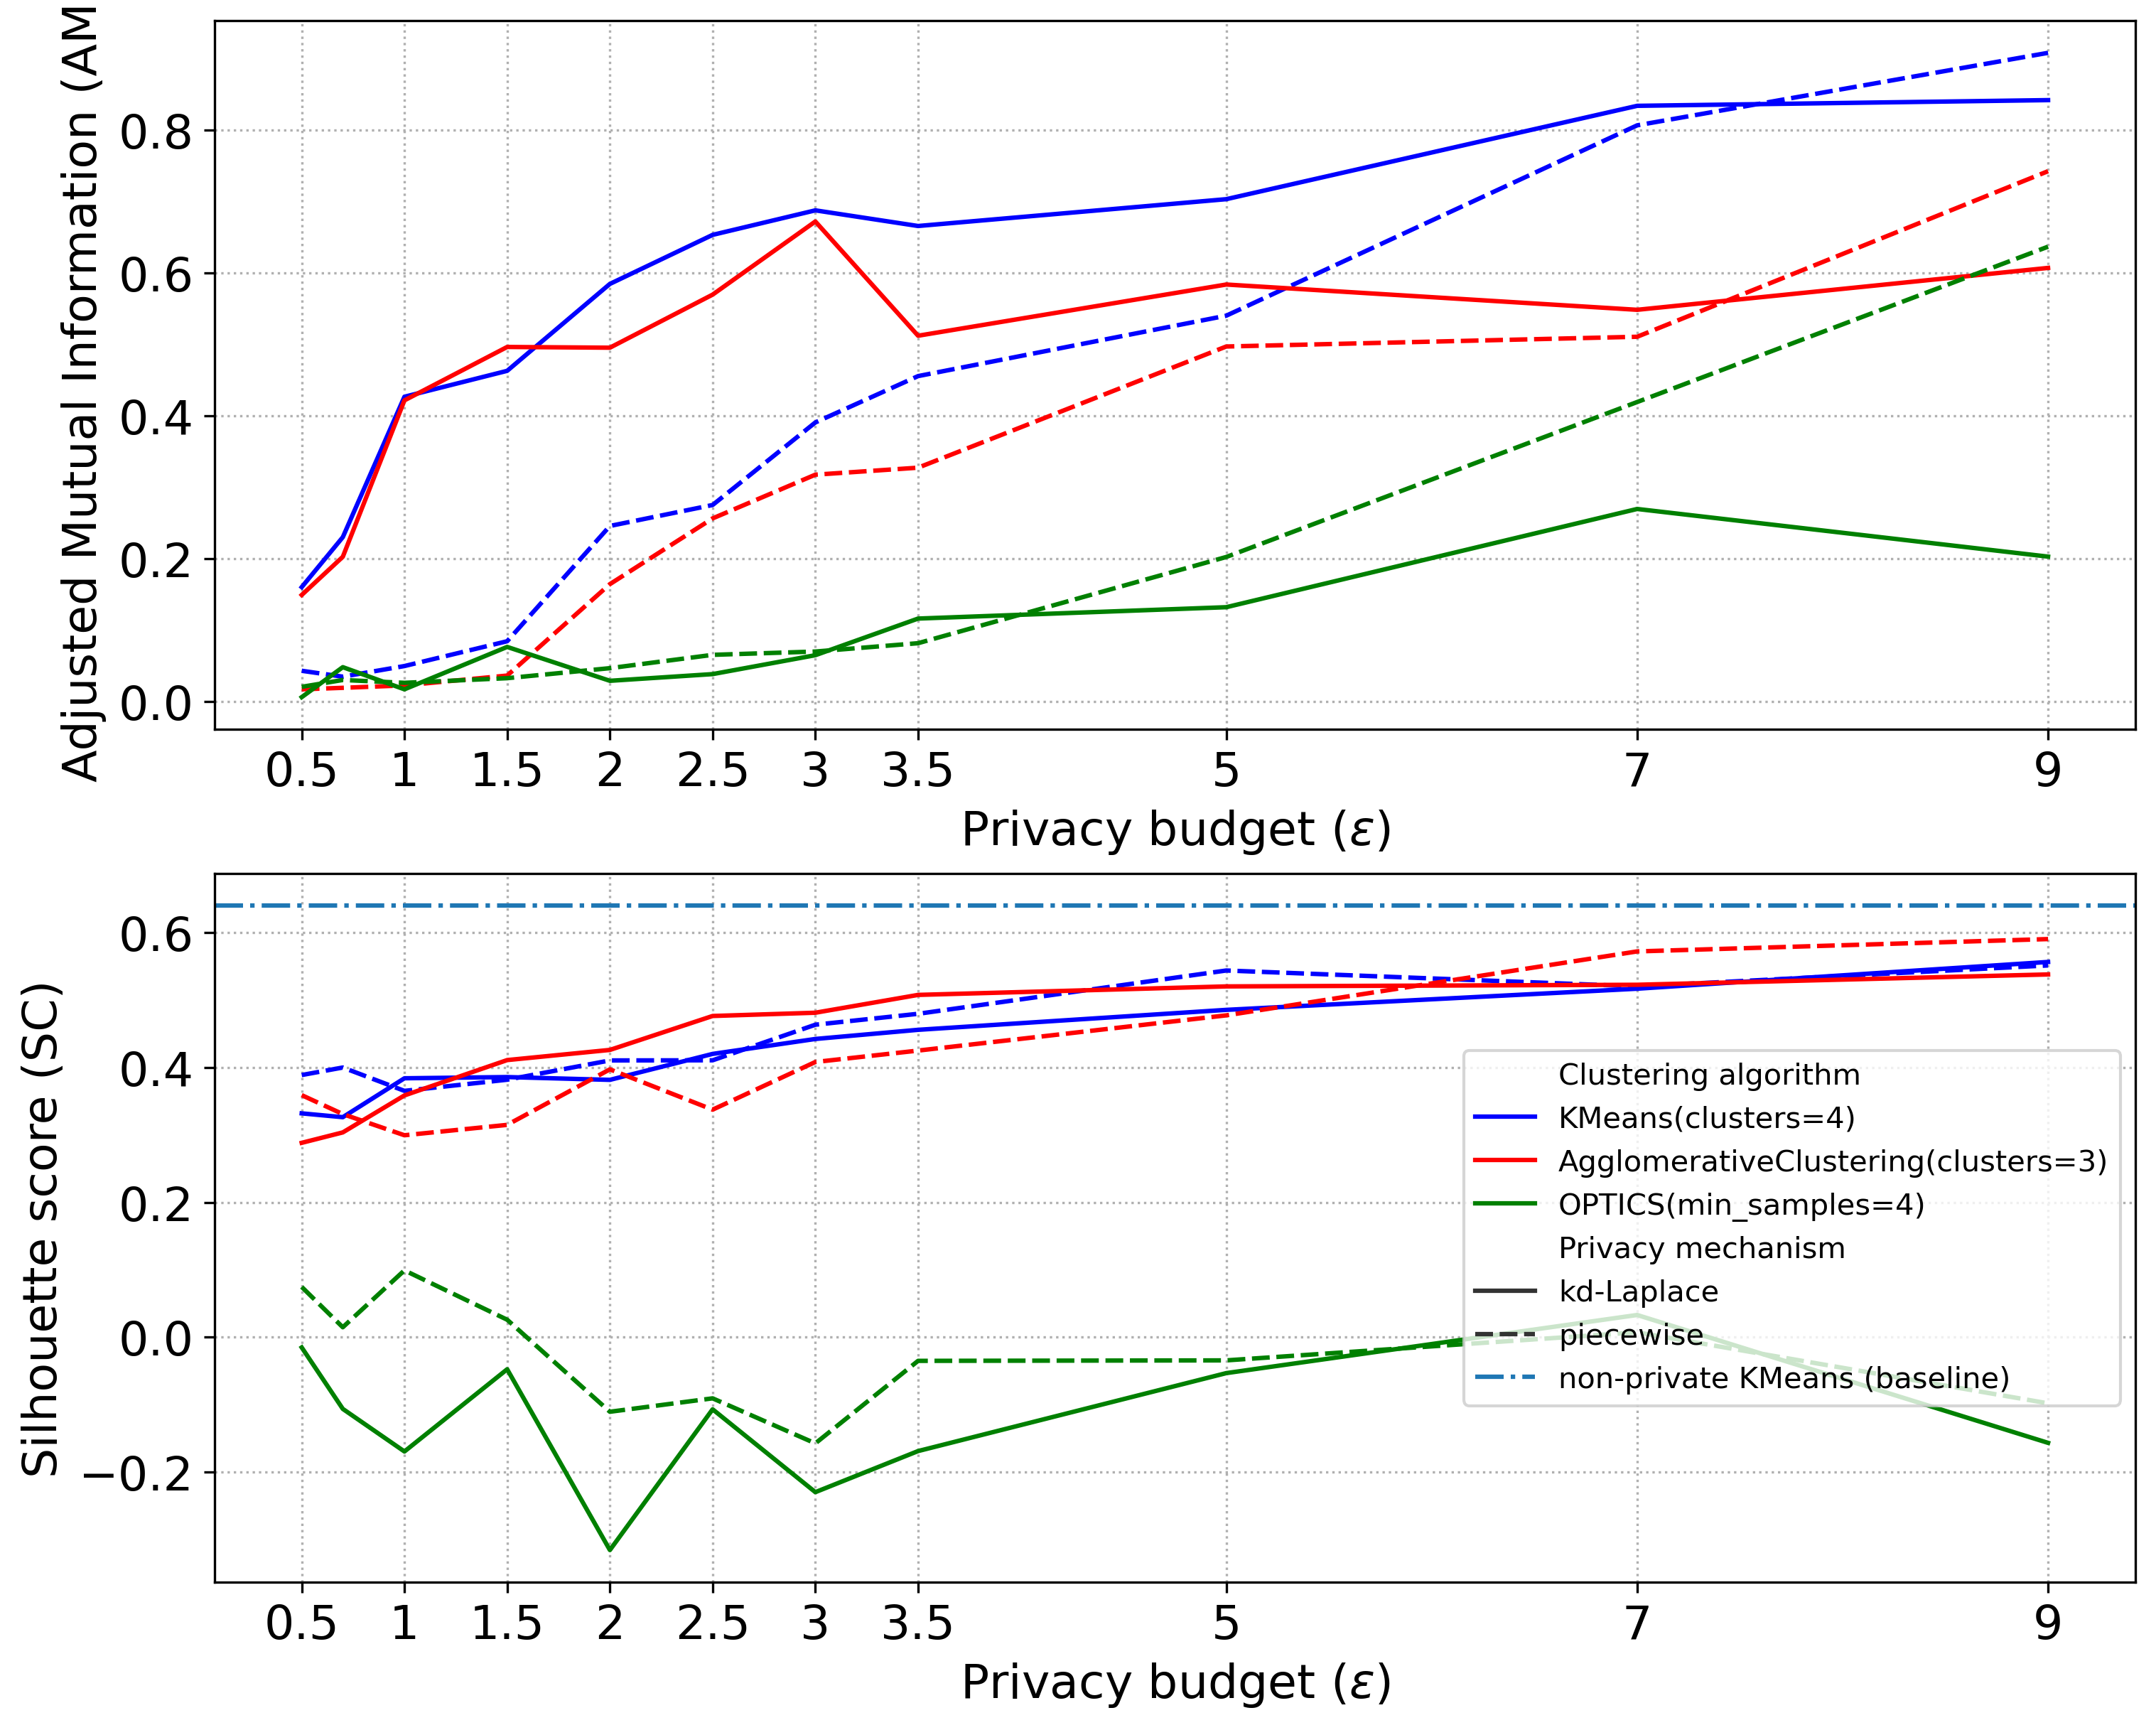
\includegraphics[width=0.65\textwidth]{Results/kd-laplace/kd-Laplace/seeds-dataset/ami-and-sc_2_dimensions.png}
            \centering
      \end{subfigure}
      \begin{subfigure}{1\textwidth}
            \centering
            \caption{\textbf{AMI (top) and SC (bottom) for the Piecewise mechanism for the 2-dimensional data seeds-dataset}}
            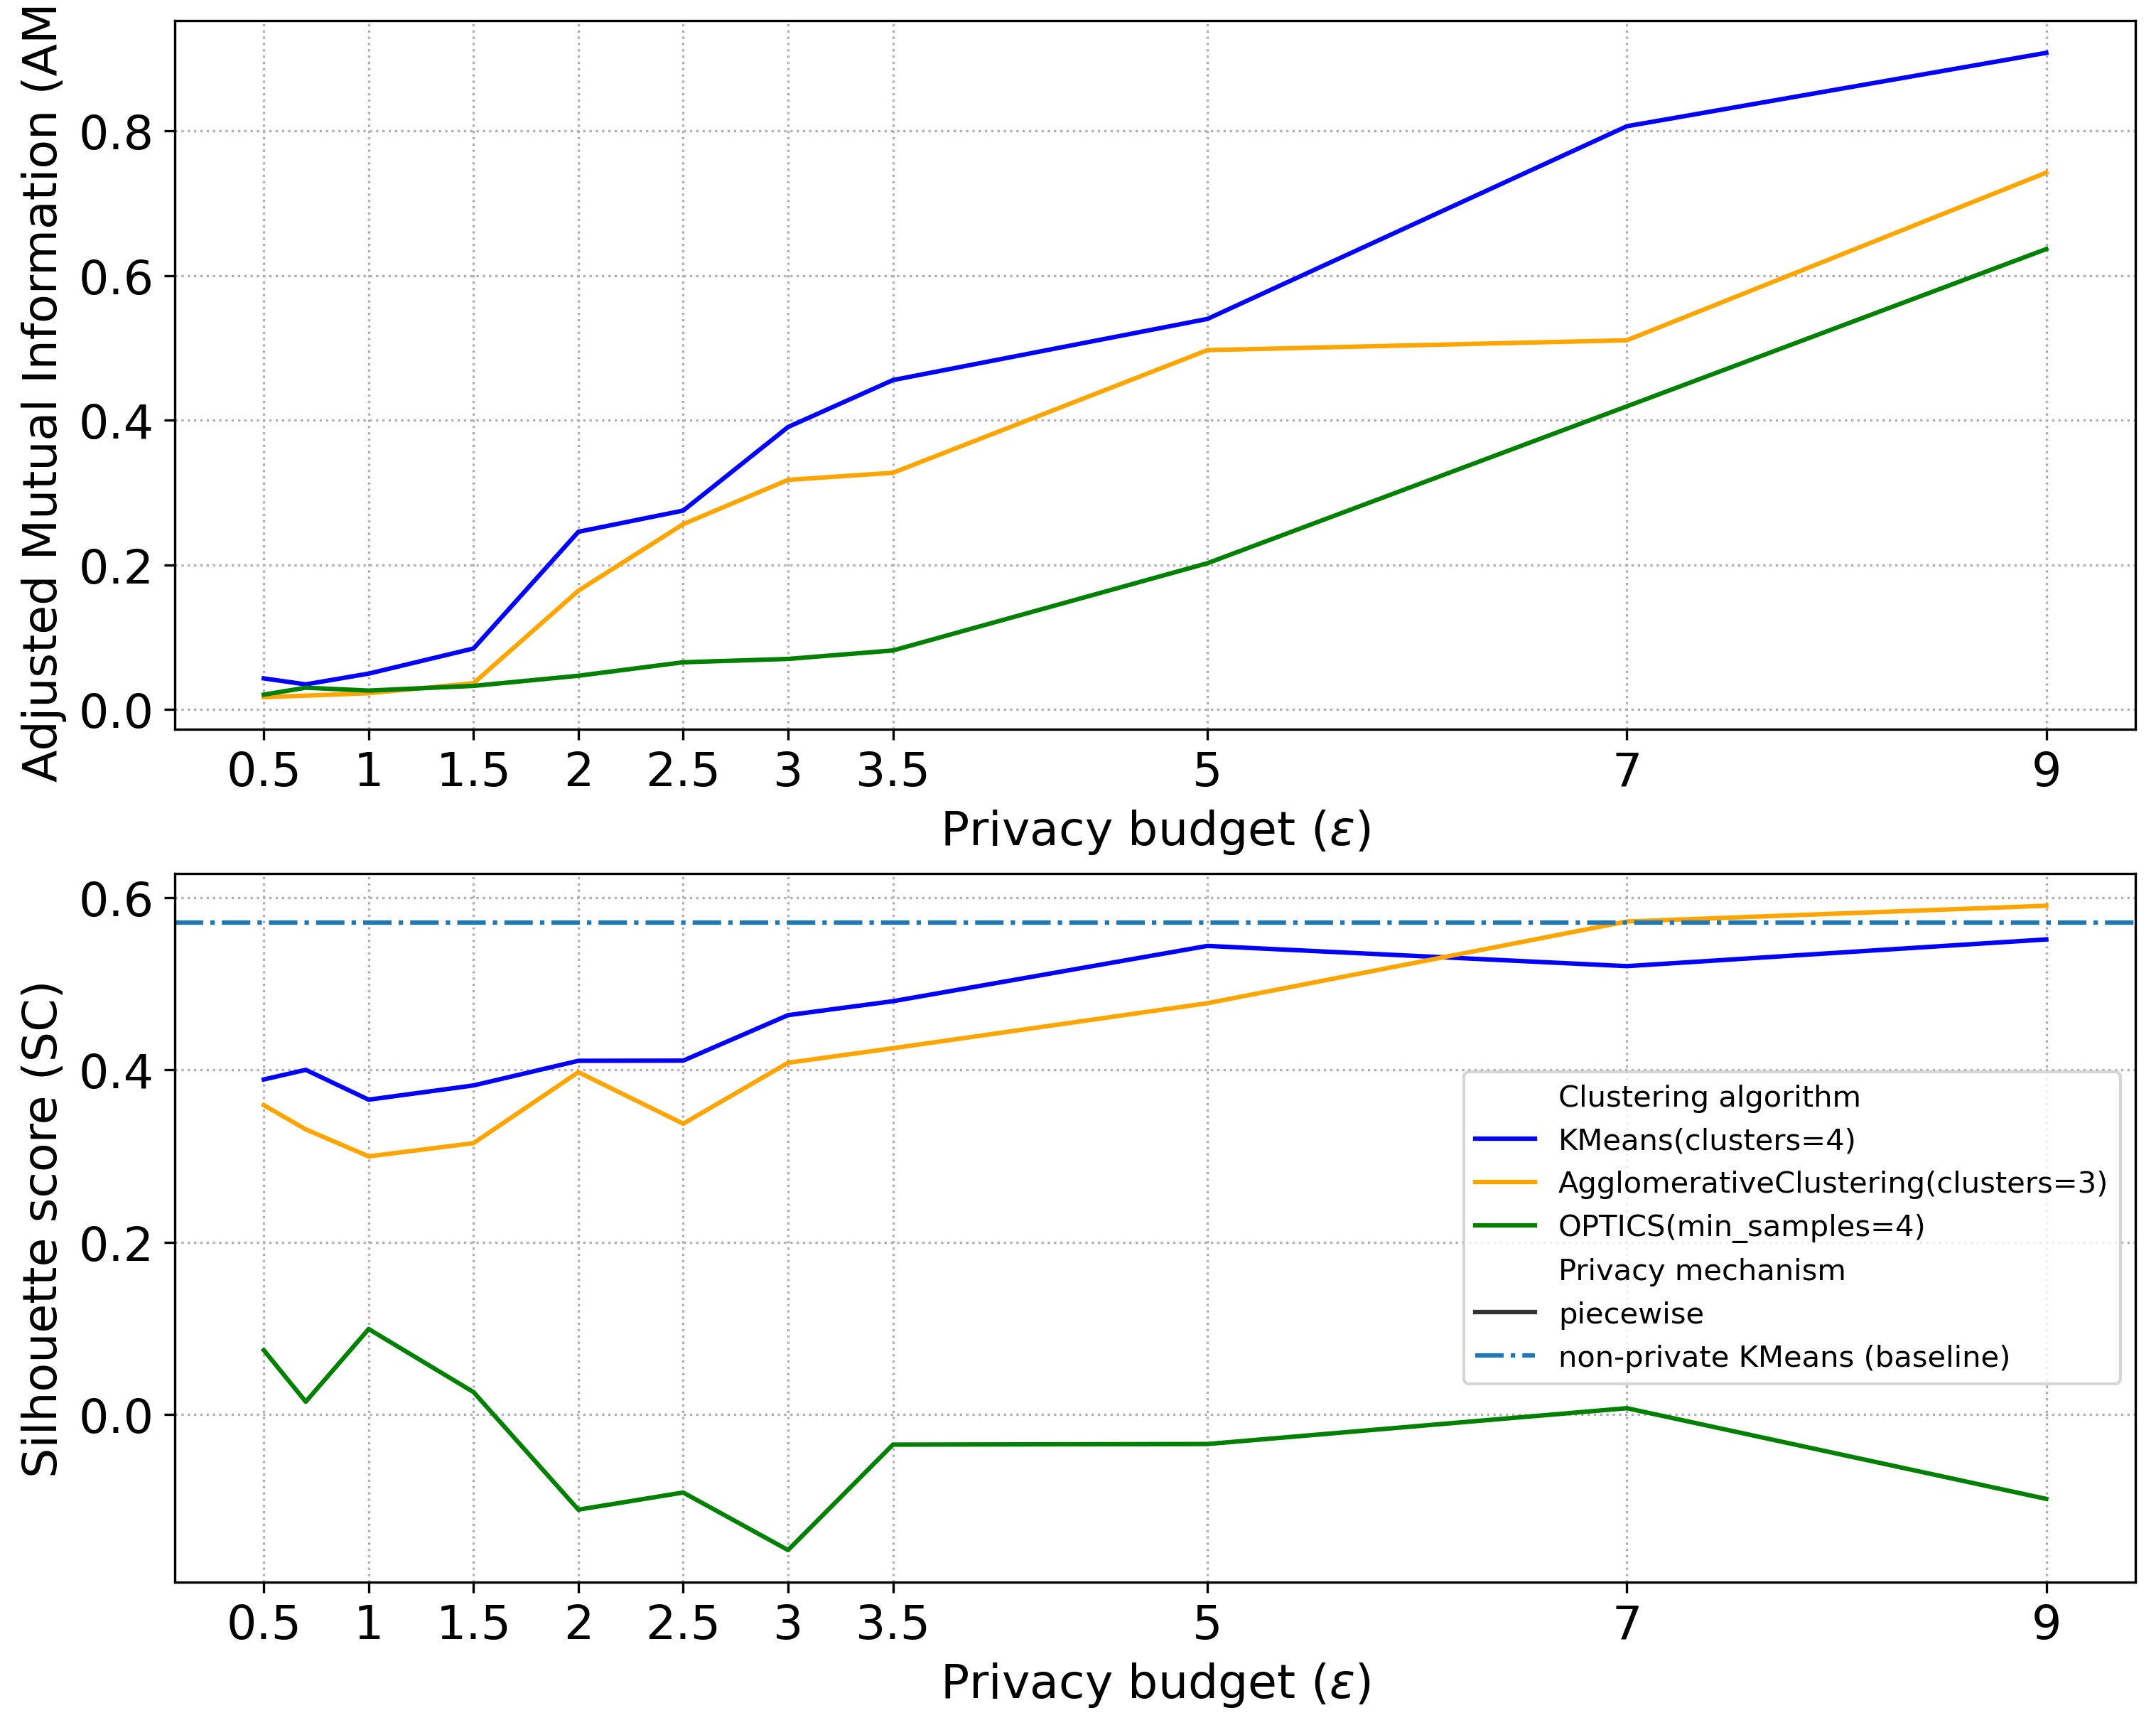
\includegraphics[width=0.65\textwidth]{Results/kd-laplace/piecewise/seeds-dataset/ami-and-sc_2_dimensions.png}
      \end{subfigure}
      \label{fig:validation-seeds-dataset_comparison_2d-laplace}
\end{figure}
%The above plots show the AMI and ARI scores for the seeds-dataset with kd-laplace/grid/optimal (left-side) and piecewise (right-side).
Piecewise shows a higher \gls{ami} for privacy budgets (epsilon) 7 and 9. In contrast, the kd-Laplace mechanism scores higher for all the other epsilons (0.1 onward 7).
K-Means achieves the best score for both mechanisms with a slight margin compared to \gls{ag}, but they score equal for \gls{sc}
For both the mechanisms, OPTICS underperforms heavily but still scores the same as AP for Piecewise.
\newpage
\begin{figure}[H]
      \centering
      \begin{subfigure}{0.3\textwidth}
            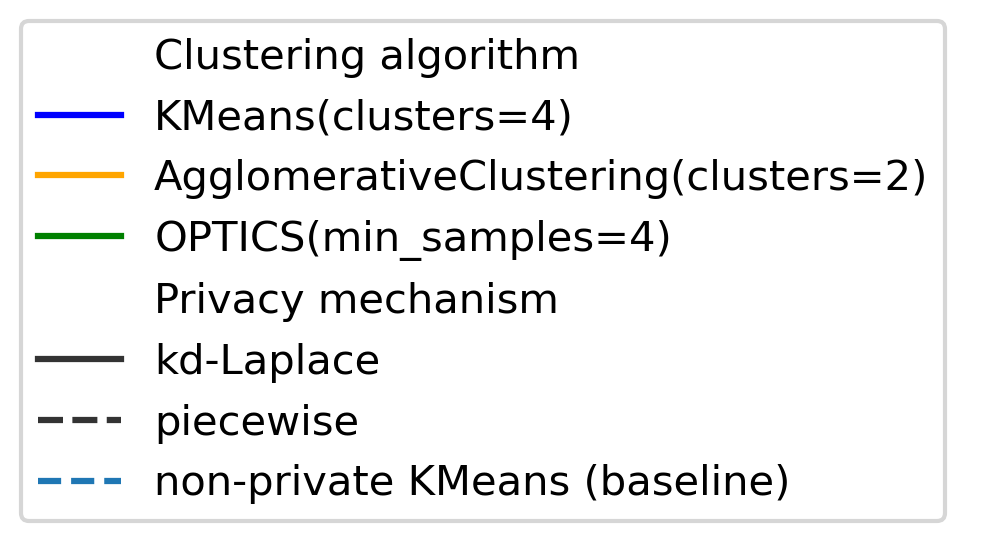
\includegraphics[width=\textwidth]{Results/kd-laplace/kd-Laplace/heart-dataset/legend_2.png}
      \end{subfigure}
      \begin{subfigure}{1\textwidth}
            \caption{\textbf{AMI (top) and SC (bottom) for the kD-Laplace mechanism for the 2-dimensional data heart-dataset}}
            \centering
            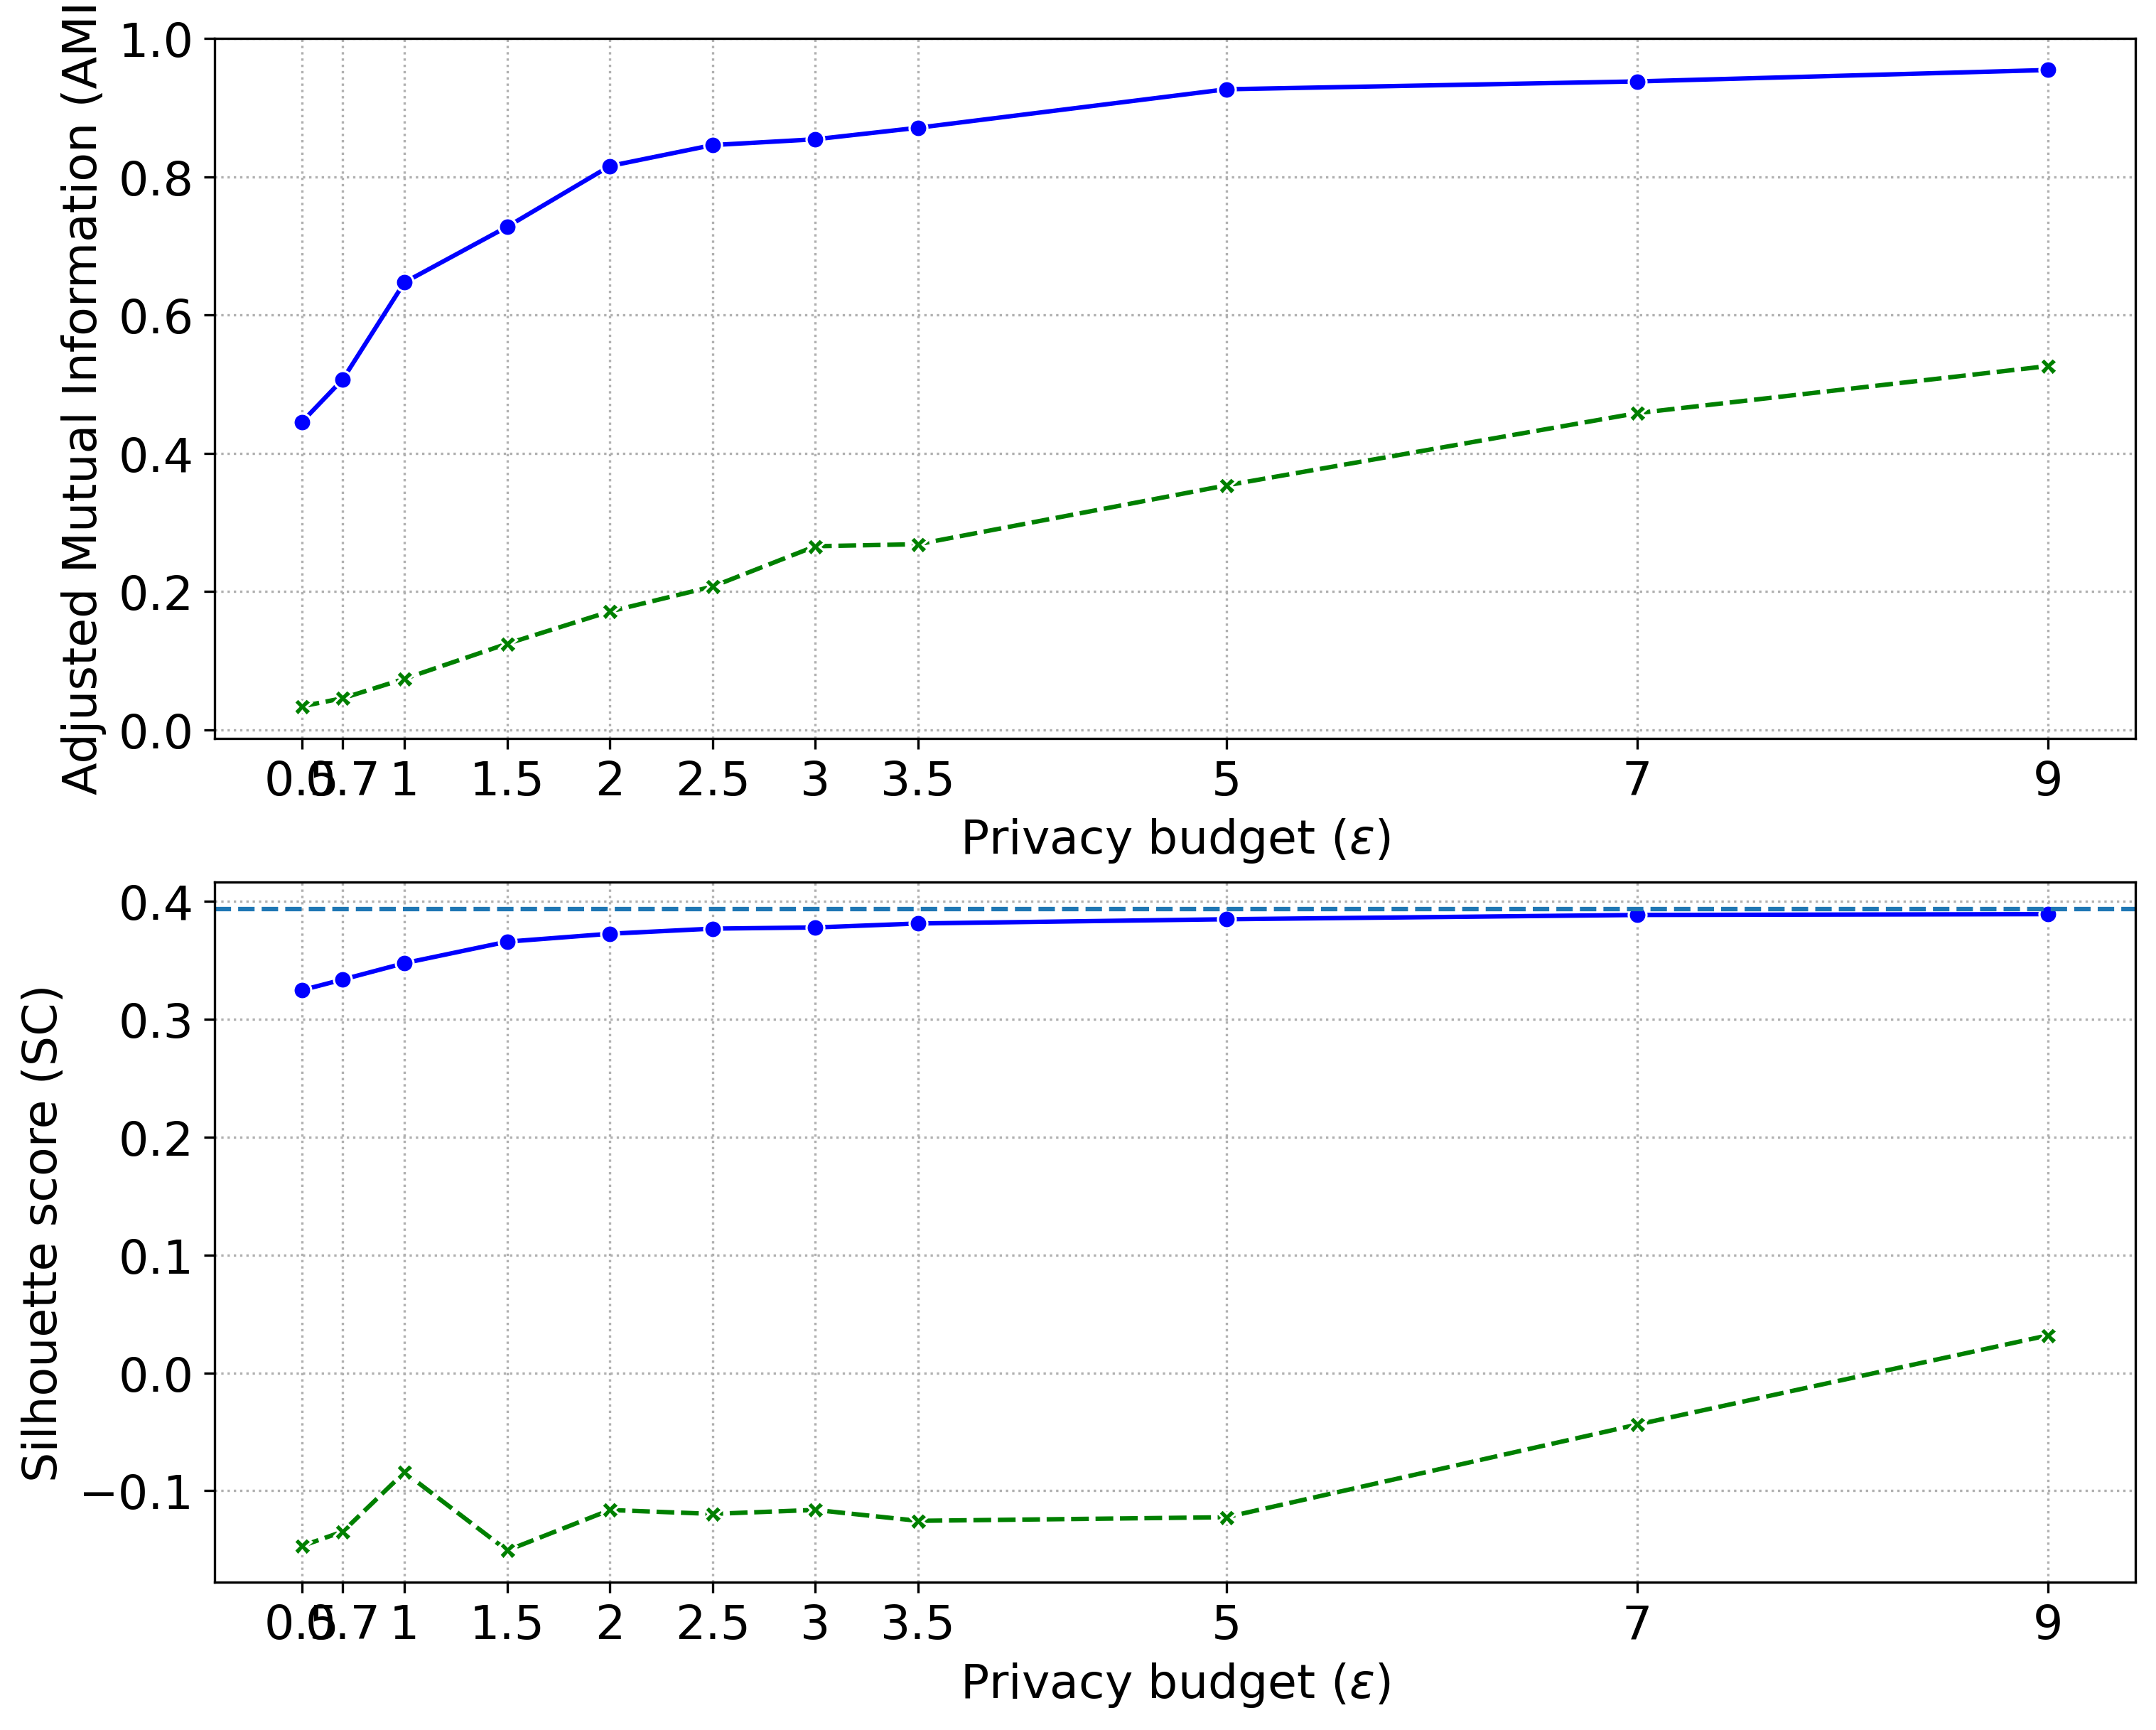
\includegraphics[width=0.65\textwidth]{Results/kd-laplace/kd-Laplace/heart-dataset/ami-and-sc_2_dimensions.png}
            \centering
      \end{subfigure}
      \begin{subfigure}{1\textwidth}
            \caption{\textbf{AMI (top) and SC (bottom) for the Piecewise mechanism for the 2-dimensional data heart-dataset}}
            \centering
            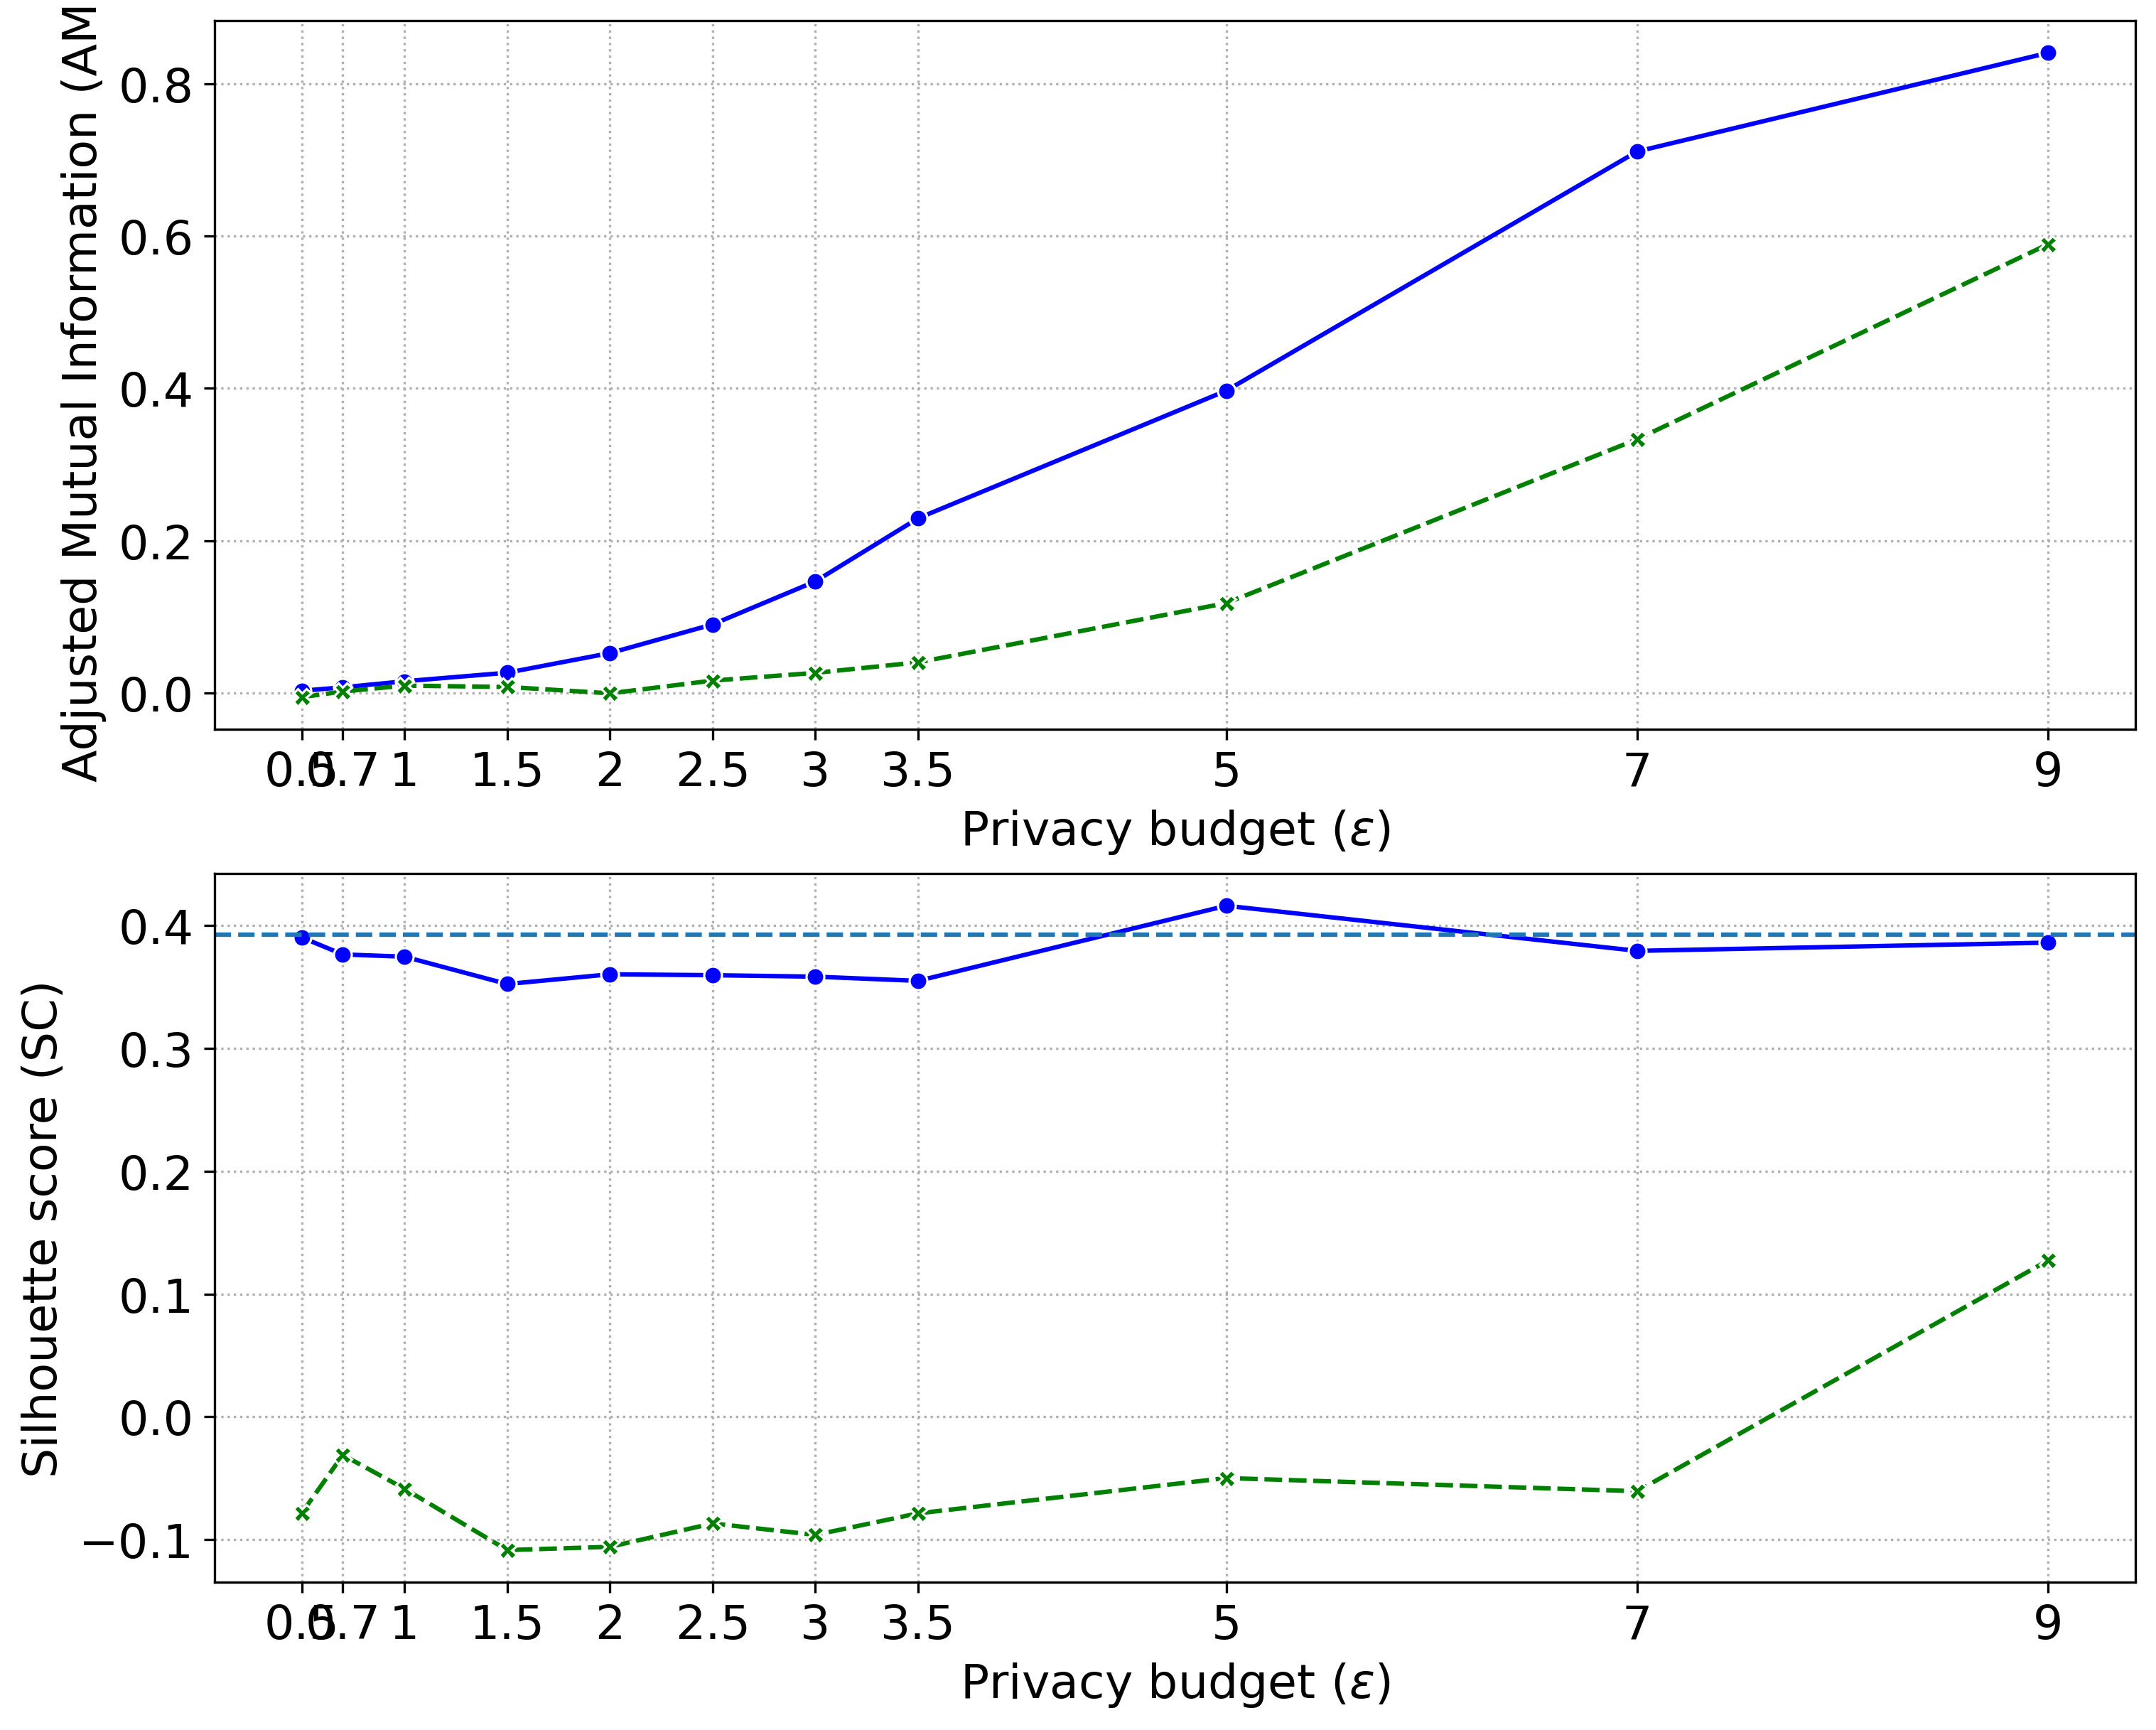
\includegraphics[width=0.65\textwidth]{Results/kd-laplace/piecewise/heart-dataset/ami-and-sc_2_dimensions.png}
      \end{subfigure}
      \label{fig:validation-heart-dataset_comparison_2d-laplace}
\end{figure}
K-Means achieves a high \gls{ami} score of 0.95+ using kD-Laplace from privacy budgets 5 to 9, compared to Piecewise scoring between 0.4 to 0.8.
Both mechanisms score high for \gls{ag} and K-Means, reaching the baseline value, but \gls{optics} performs poorly.
\gls{ag} fluctuates more with kD-Laplace. For \gls{sc}, both kD-Laplace and Piecewise reach the baseline for \gls{ag} and K-Means, while \gls{optics} performs poorly.
\newpage
\begin{figure}[H]
      \centering
      \begin{subfigure}{0.3\textwidth}
            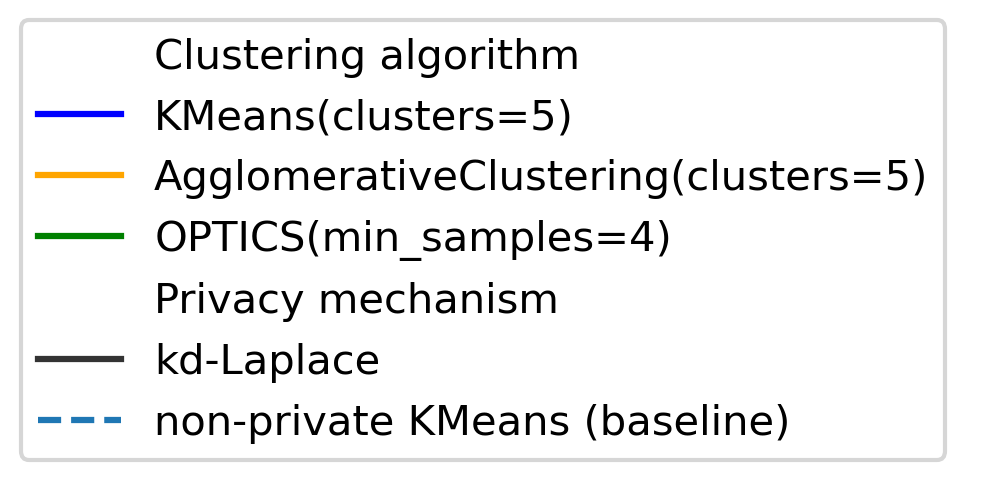
\includegraphics[width=\textwidth]{Results/kd-laplace/kd-Laplace/circle-dataset/legend_2.png}
      \end{subfigure}
      \begin{subfigure}{1\textwidth}
            \centering
            \caption{\textbf{AMI (top) and SC (bottom) for the kD-Laplace mechanism for the 2-dimensional data circle-dataset}}
            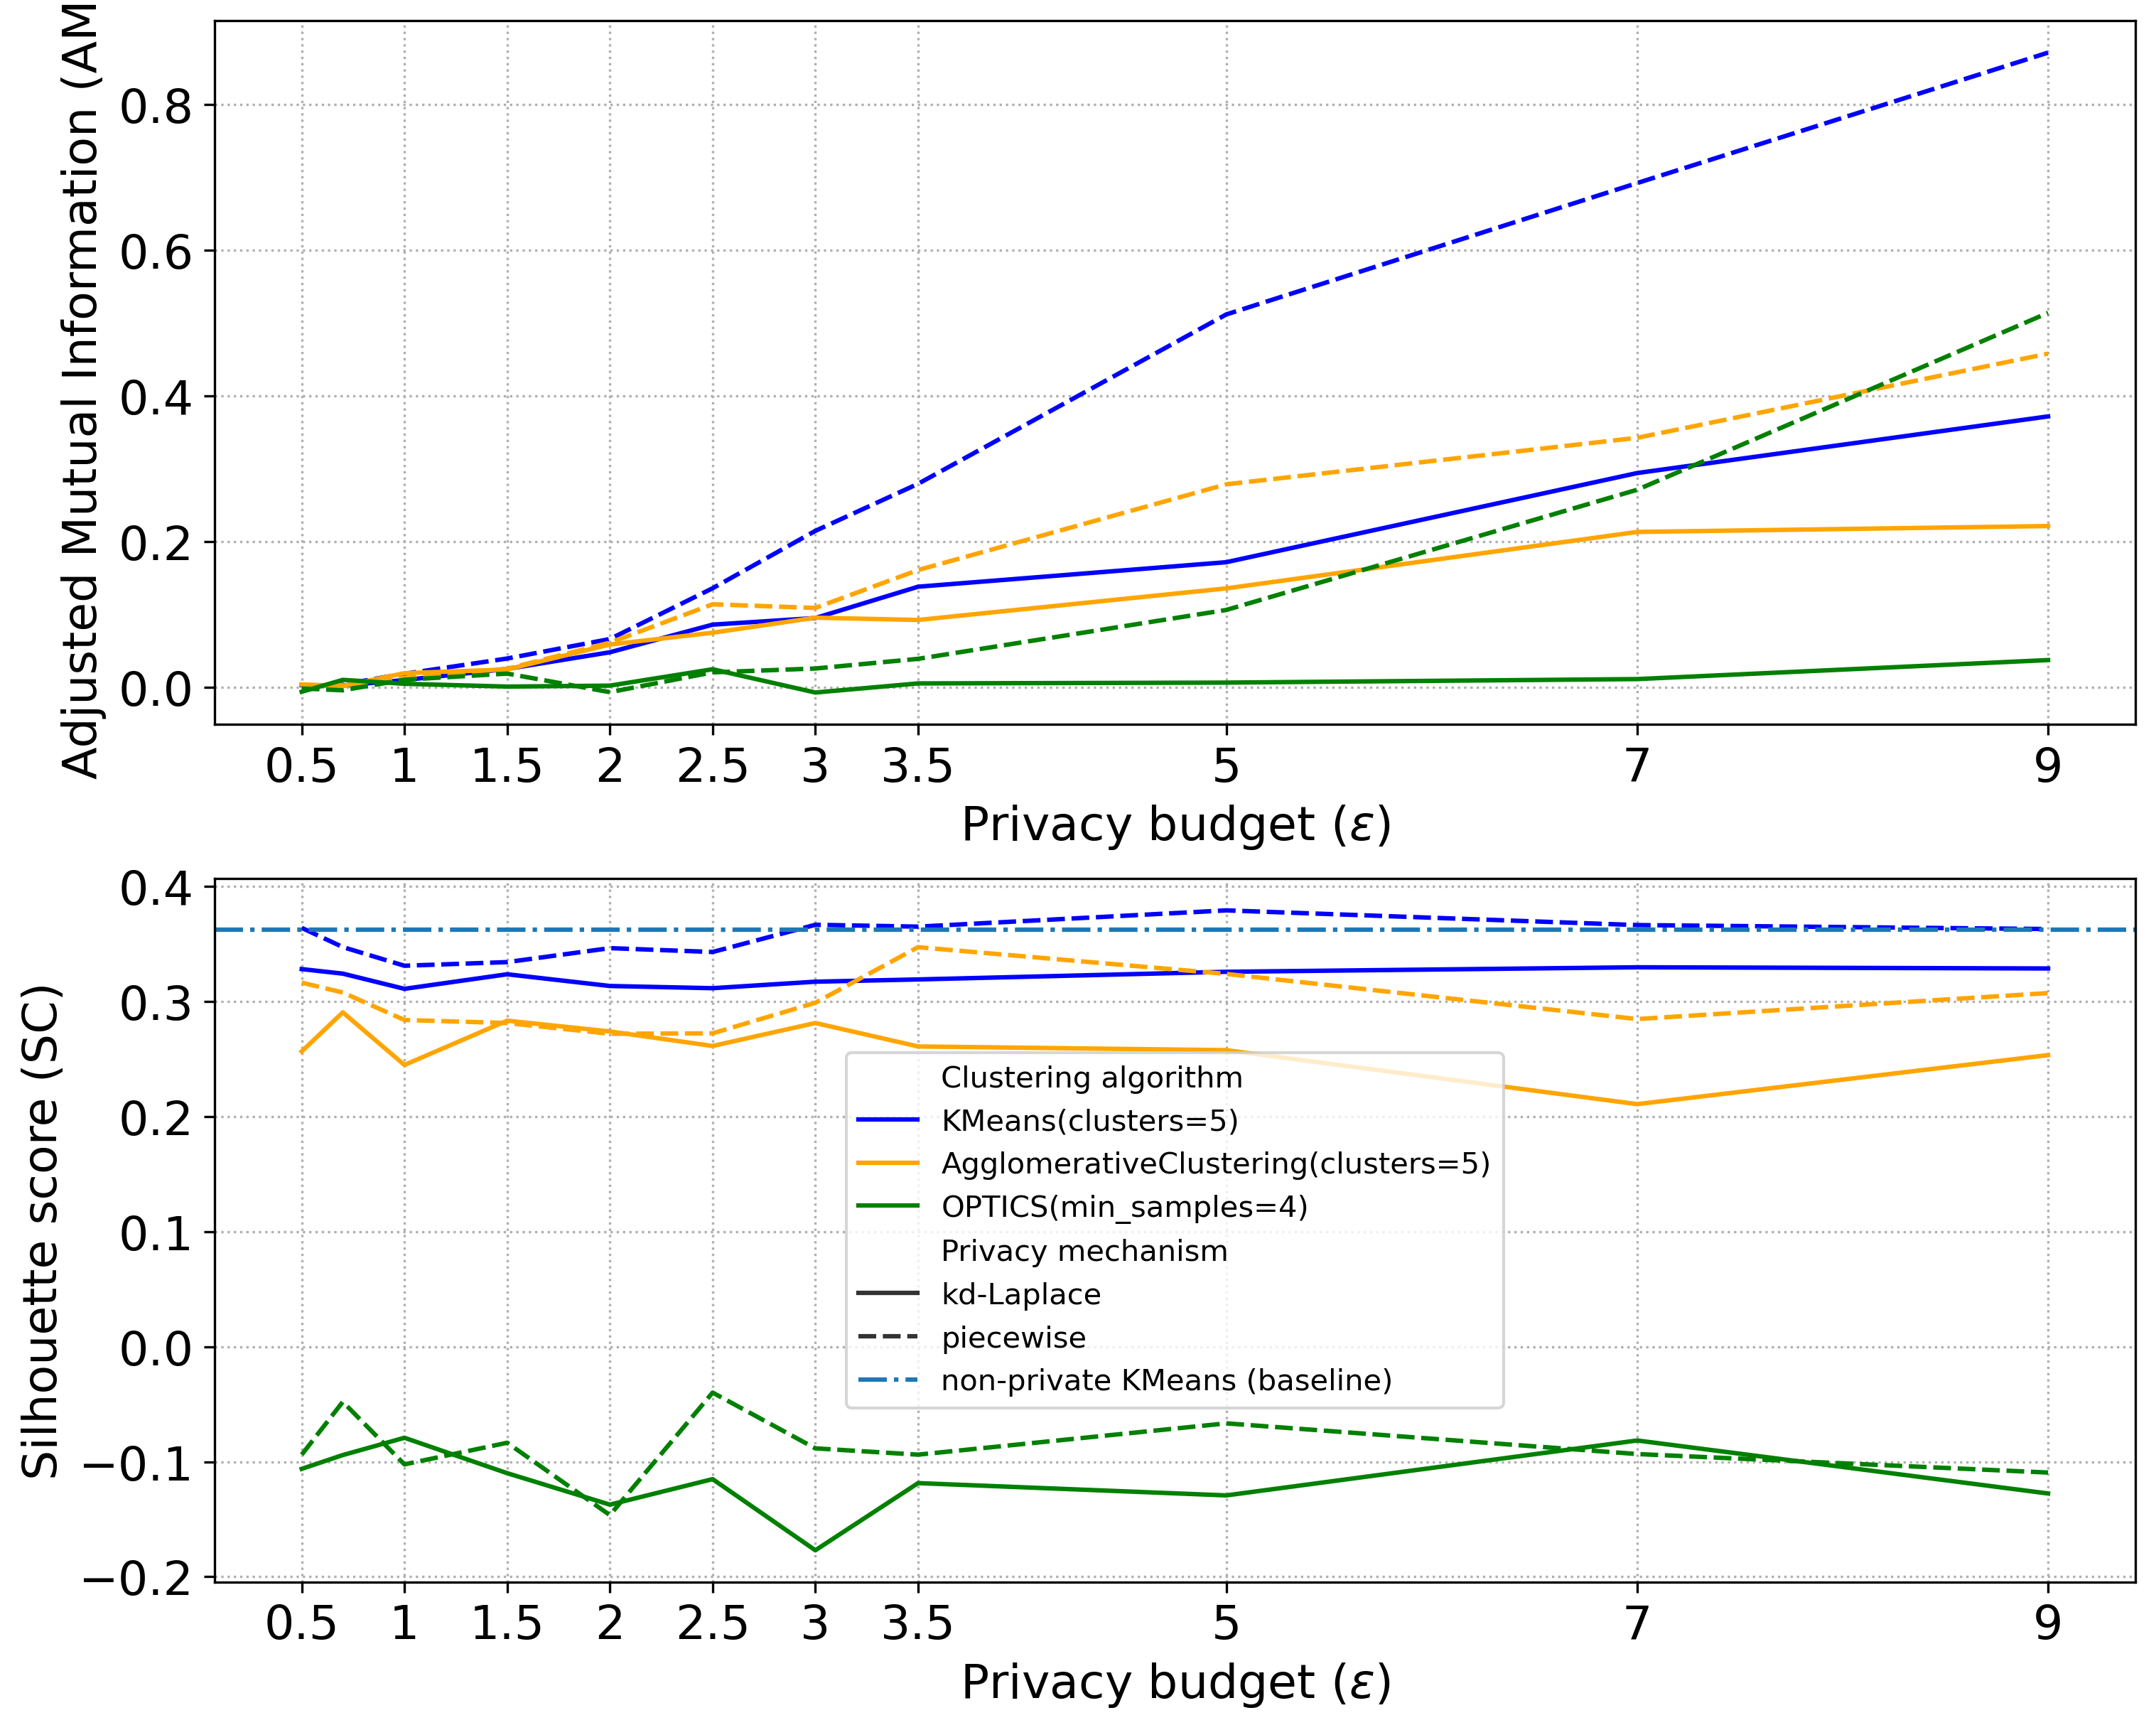
\includegraphics[width=0.65\textwidth]{Results/kd-laplace/kd-Laplace/circle-dataset/ami-and-sc_2_dimensions.png}
            \centering
      \end{subfigure}
      \begin{subfigure}{1\textwidth}
            \centering
            \caption{\textbf{AMI (top) and SC (bottom) for the Piecewise mechanism for the 2-dimensional data circle-dataset}}
            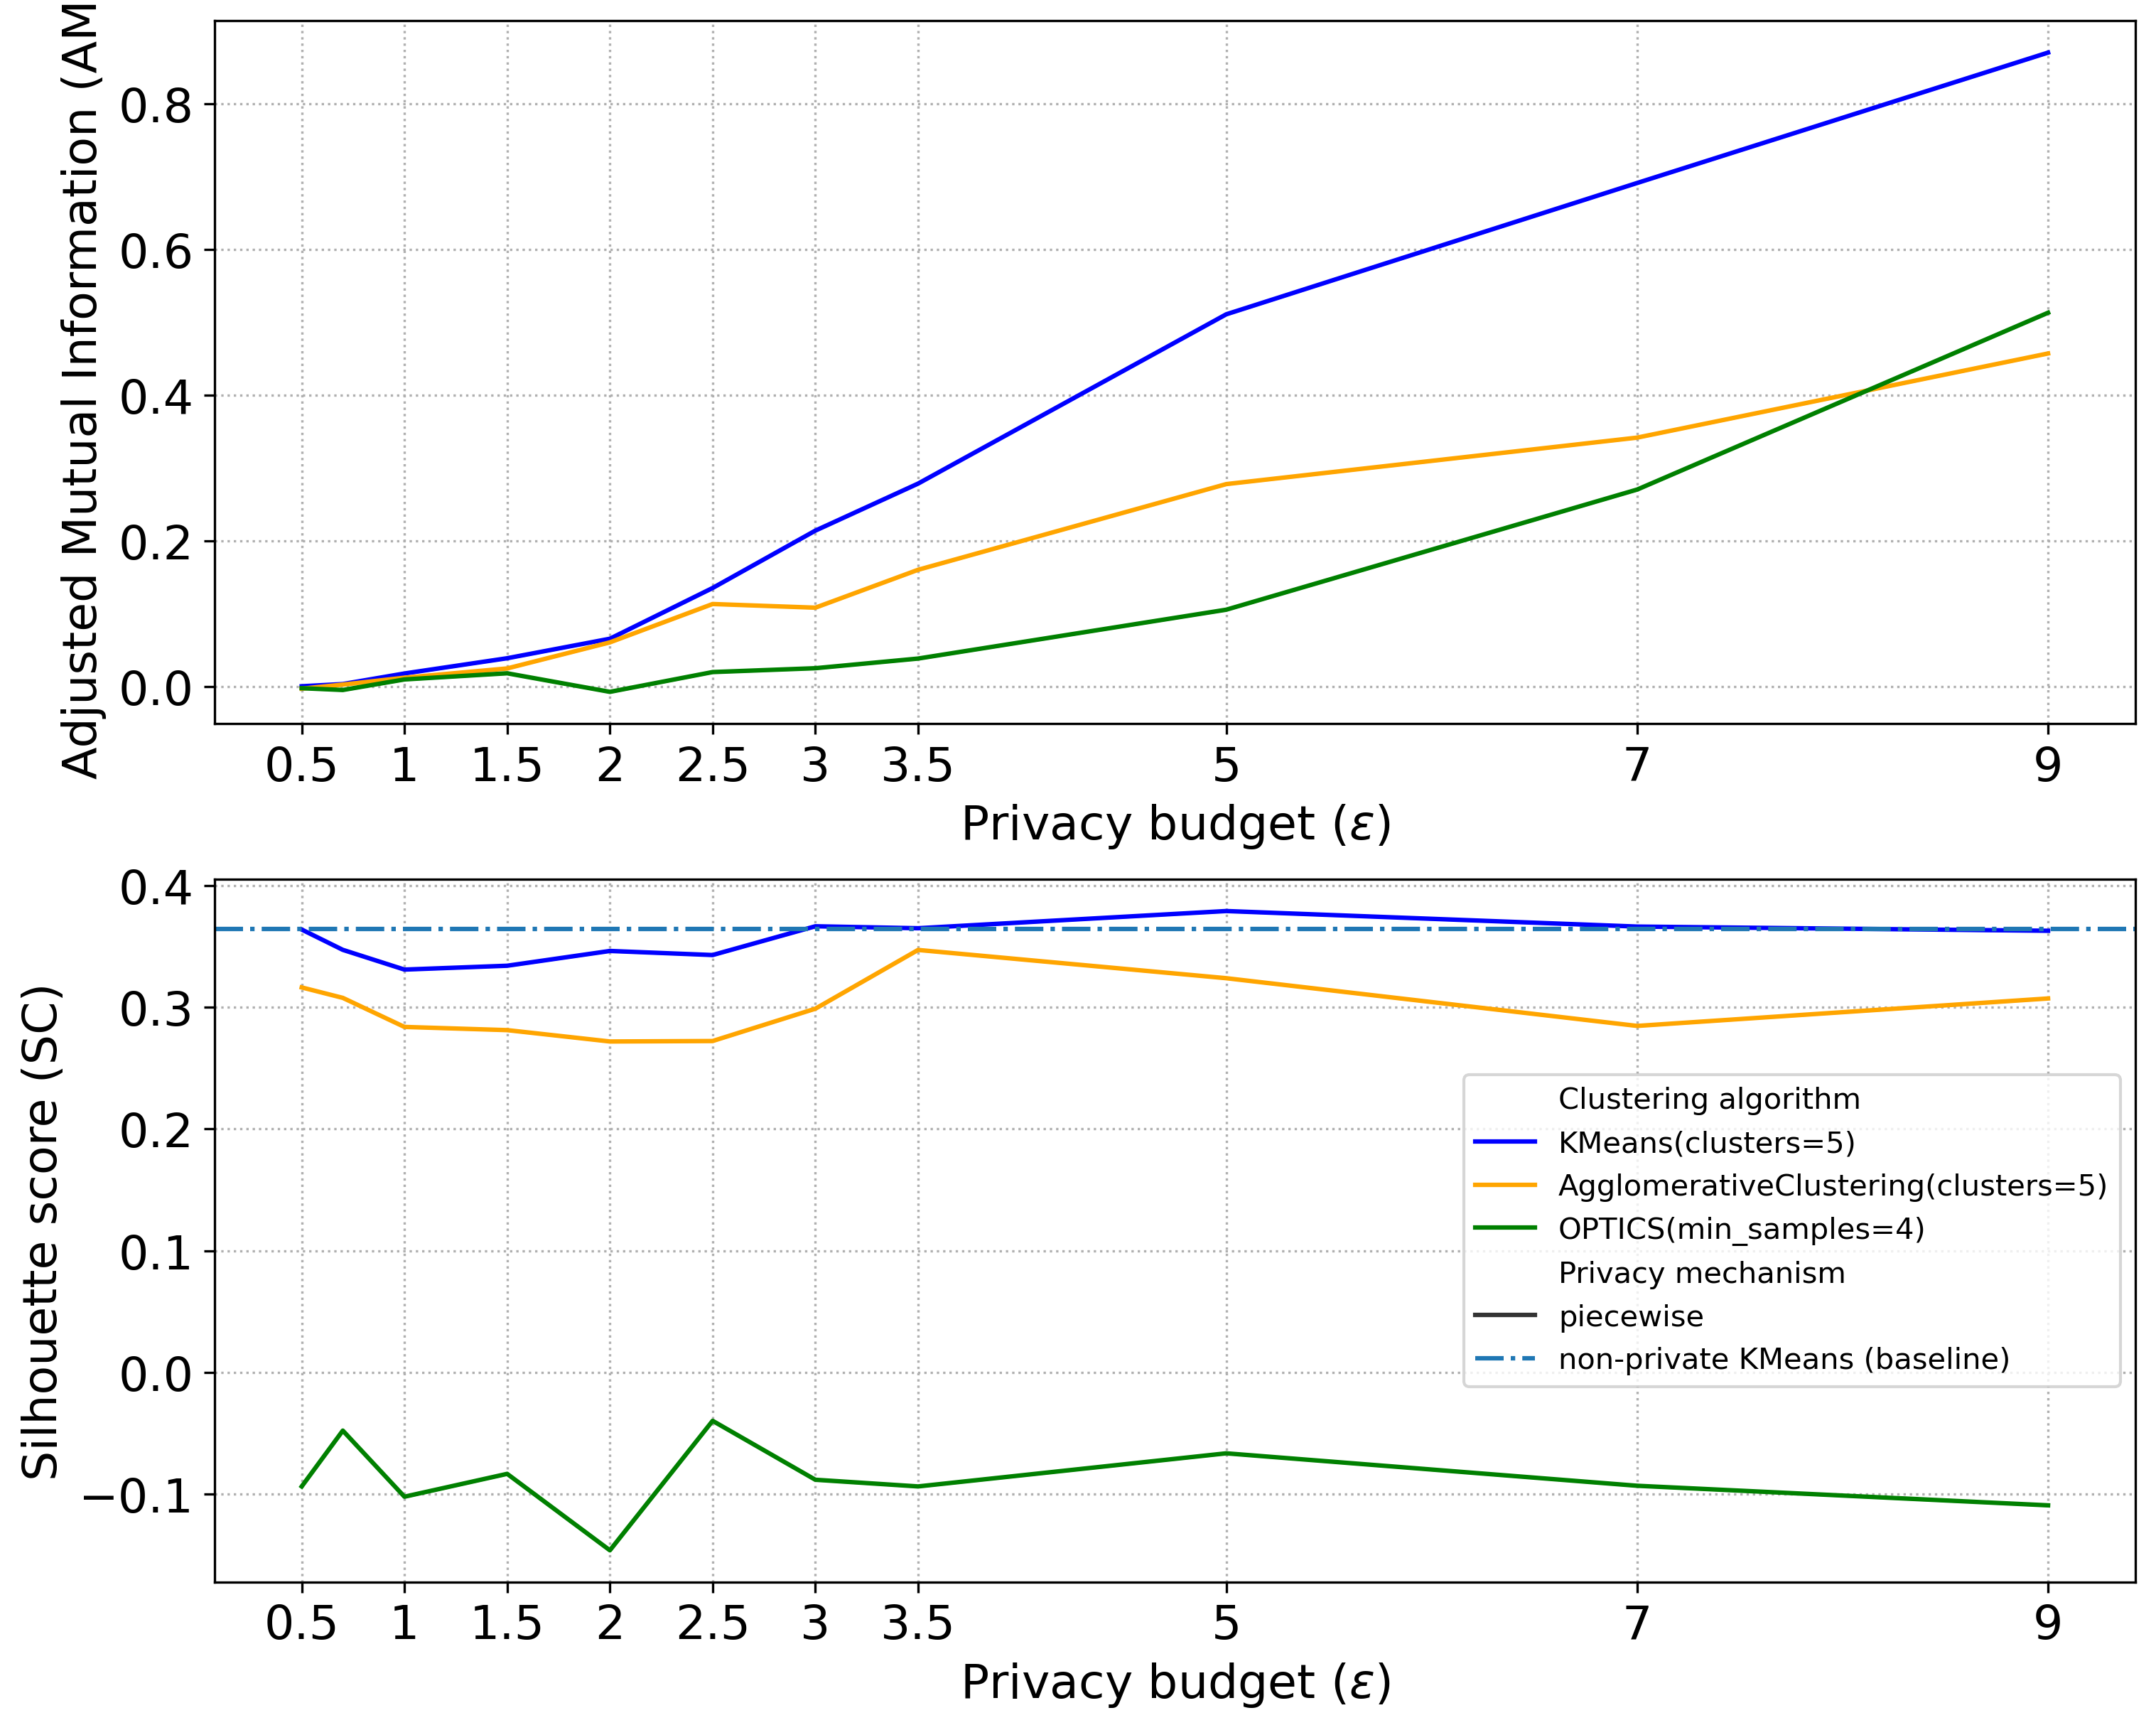
\includegraphics[width=0.65\textwidth]{Results/kd-laplace/piecewise/circle-dataset/ami-and-sc_2_dimensions.png}
      \end{subfigure}
      \label{fig:validation-circle-dataset_comparison_2d-laplace}
\end{figure}
For both mechanisms, K-Means scores the privacy budgets from 2.5.
Compared to Piecewise, the kD-Laplace mechanism scores the worst overall for almost all privacy budgets.
The Piecewise algorithm scores 0.84 as the highest \gls{ami} for K-Means, while kd-Laplace scores 0.36.
The difference is a little less for \gls{sc}, but overall Piecewise is 0.10 higher.
K-Means is for Piecewise on the baseline value for privacy budgets 3 to 9.
\newpage
\begin{figure}[H]
      \centering
      \begin{subfigure}{0.3\textwidth}
            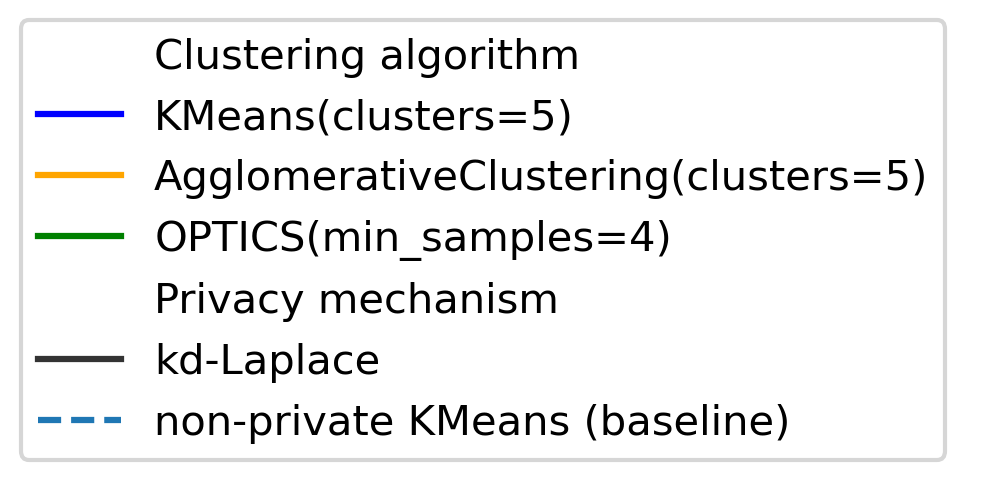
\includegraphics[width=\textwidth]{Results/kd-laplace/kd-Laplace/circle-dataset/legend_2.png}
      \end{subfigure}
      \begin{subfigure}{1\textwidth}
            \centering
            \caption{\textbf{AMI (top) and SC (bottom) for the kD-Laplace mechanism for the 2-dimensional data line-dataset}}
            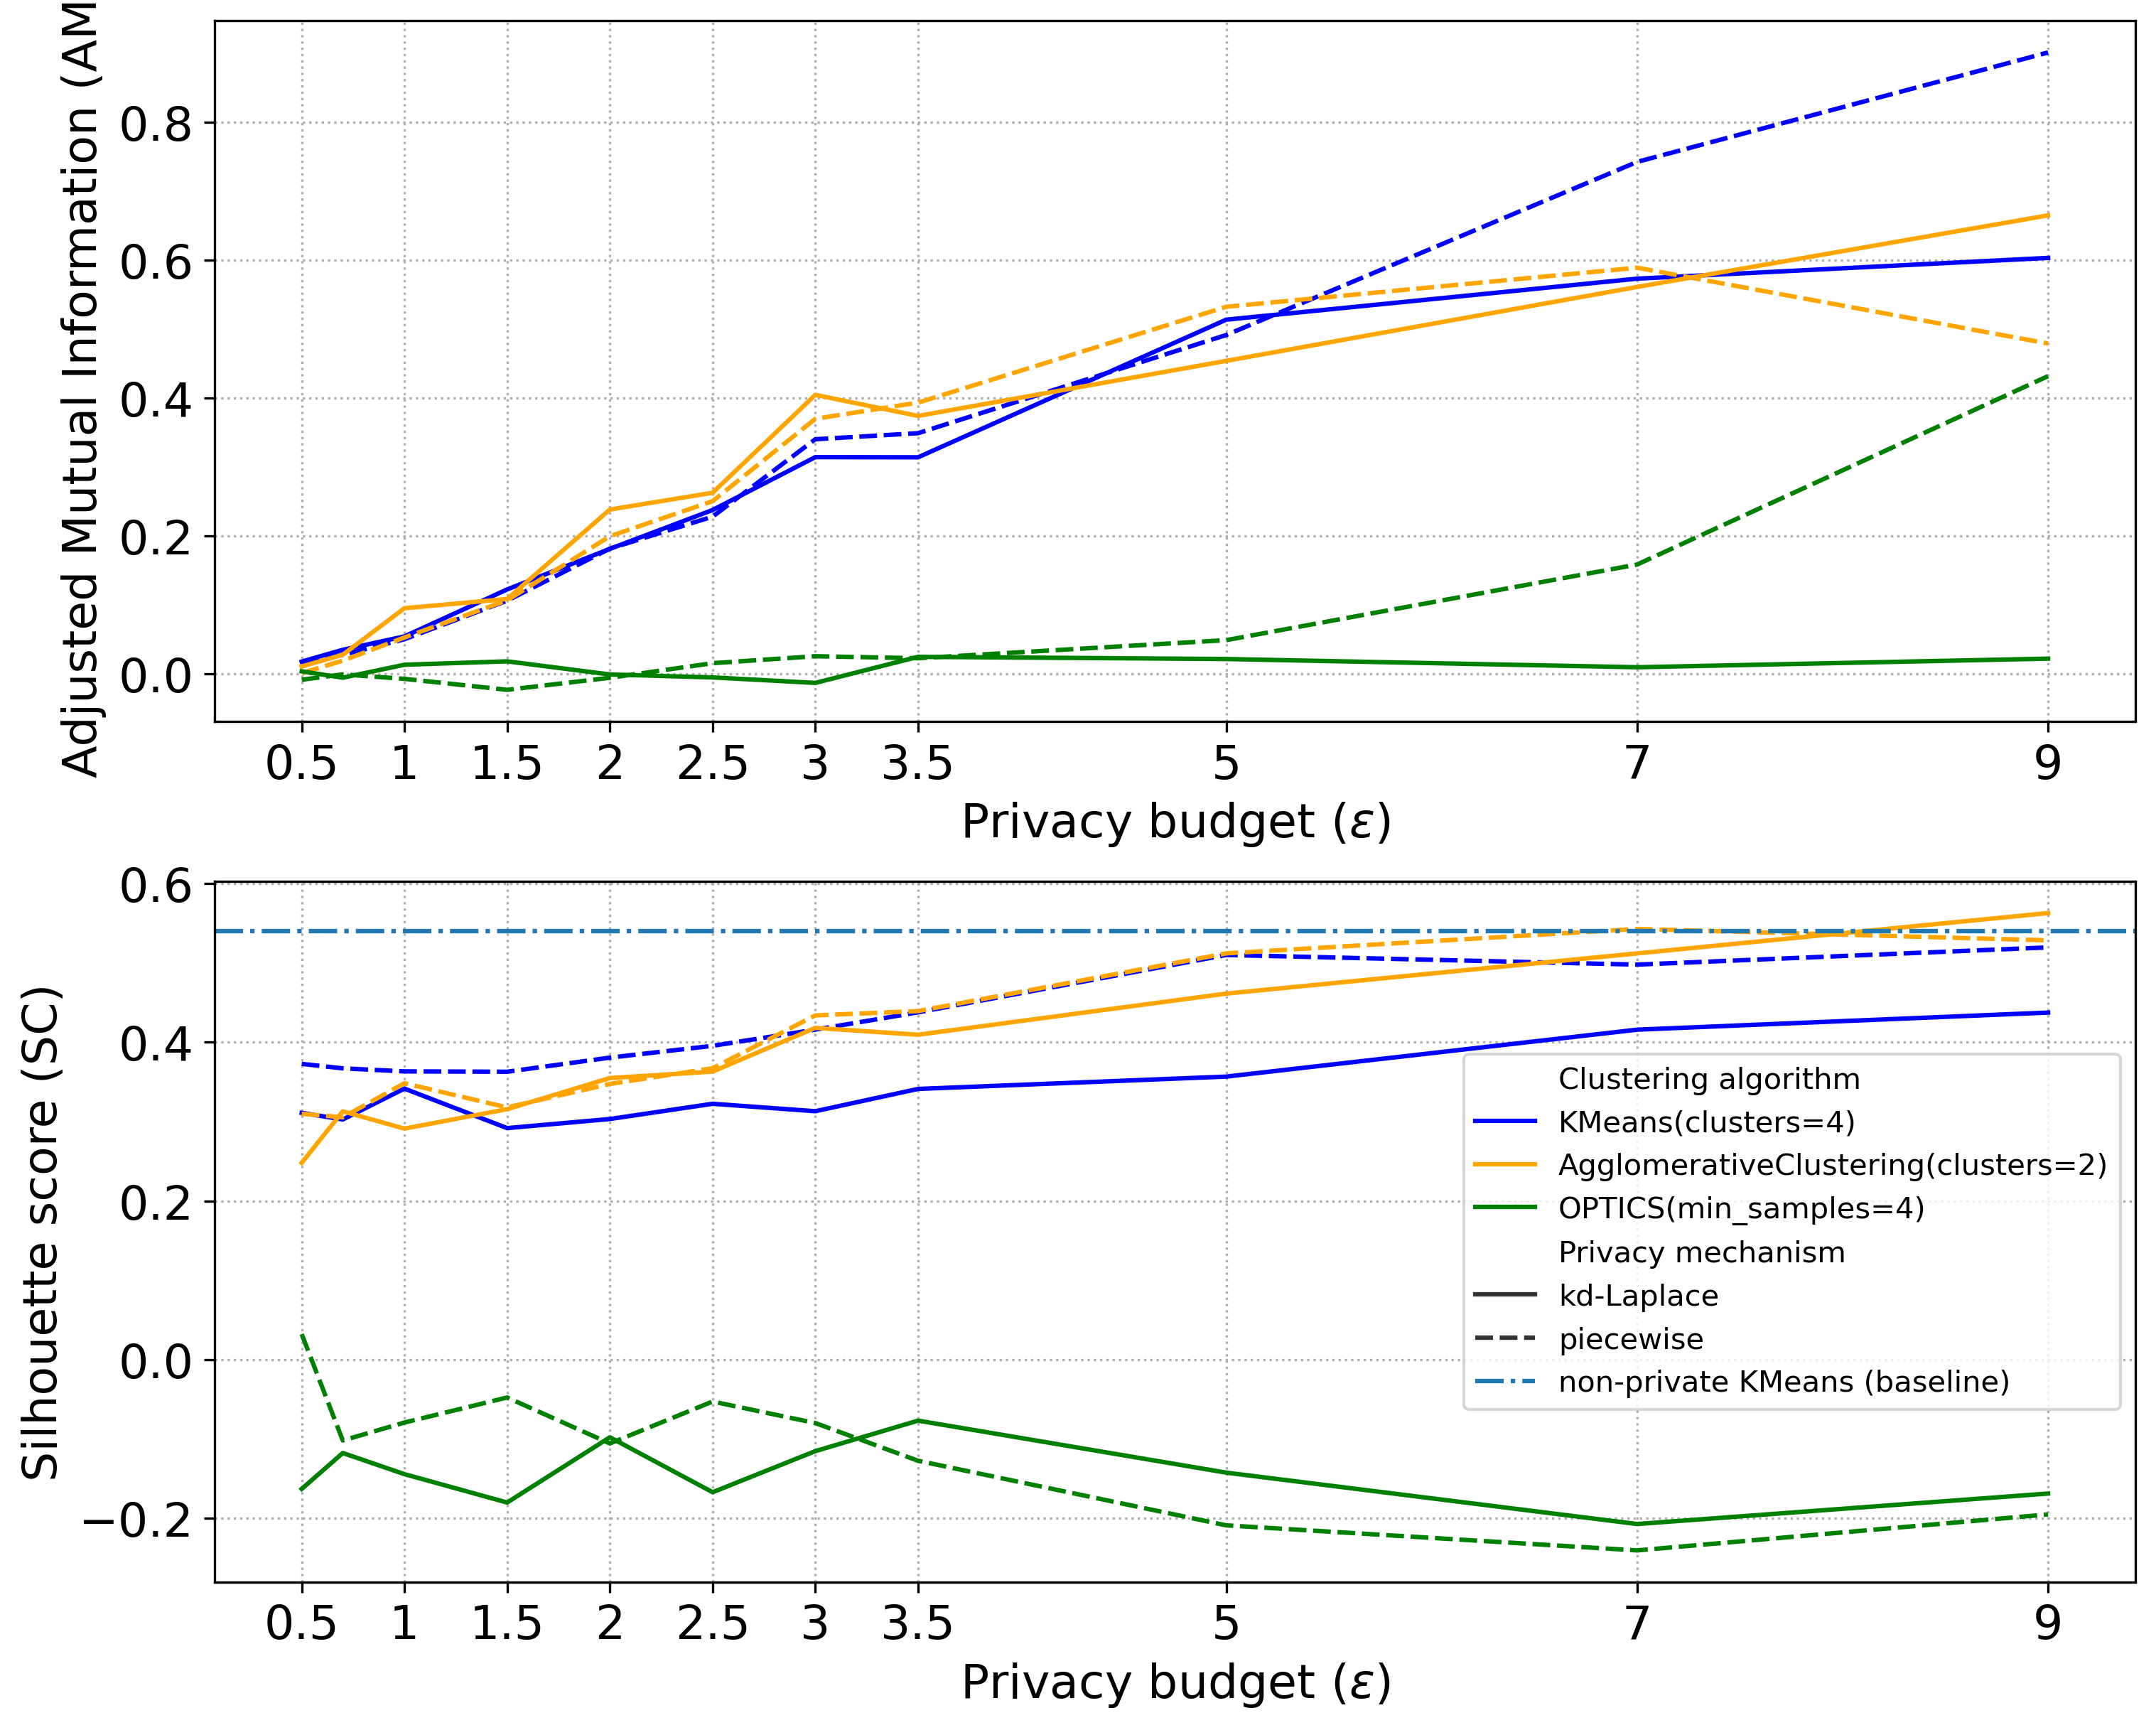
\includegraphics[width=0.65\textwidth]{Results/kd-laplace/kd-Laplace/line-dataset/ami-and-sc_2_dimensions.png}
            \centering
      \end{subfigure}
      \begin{subfigure}{1\textwidth}
            \centering
            \caption{\textbf{AMI (top) and SC (bottom) for the Piecewise mechanism for the 2-dimensional data line-dataset}}
            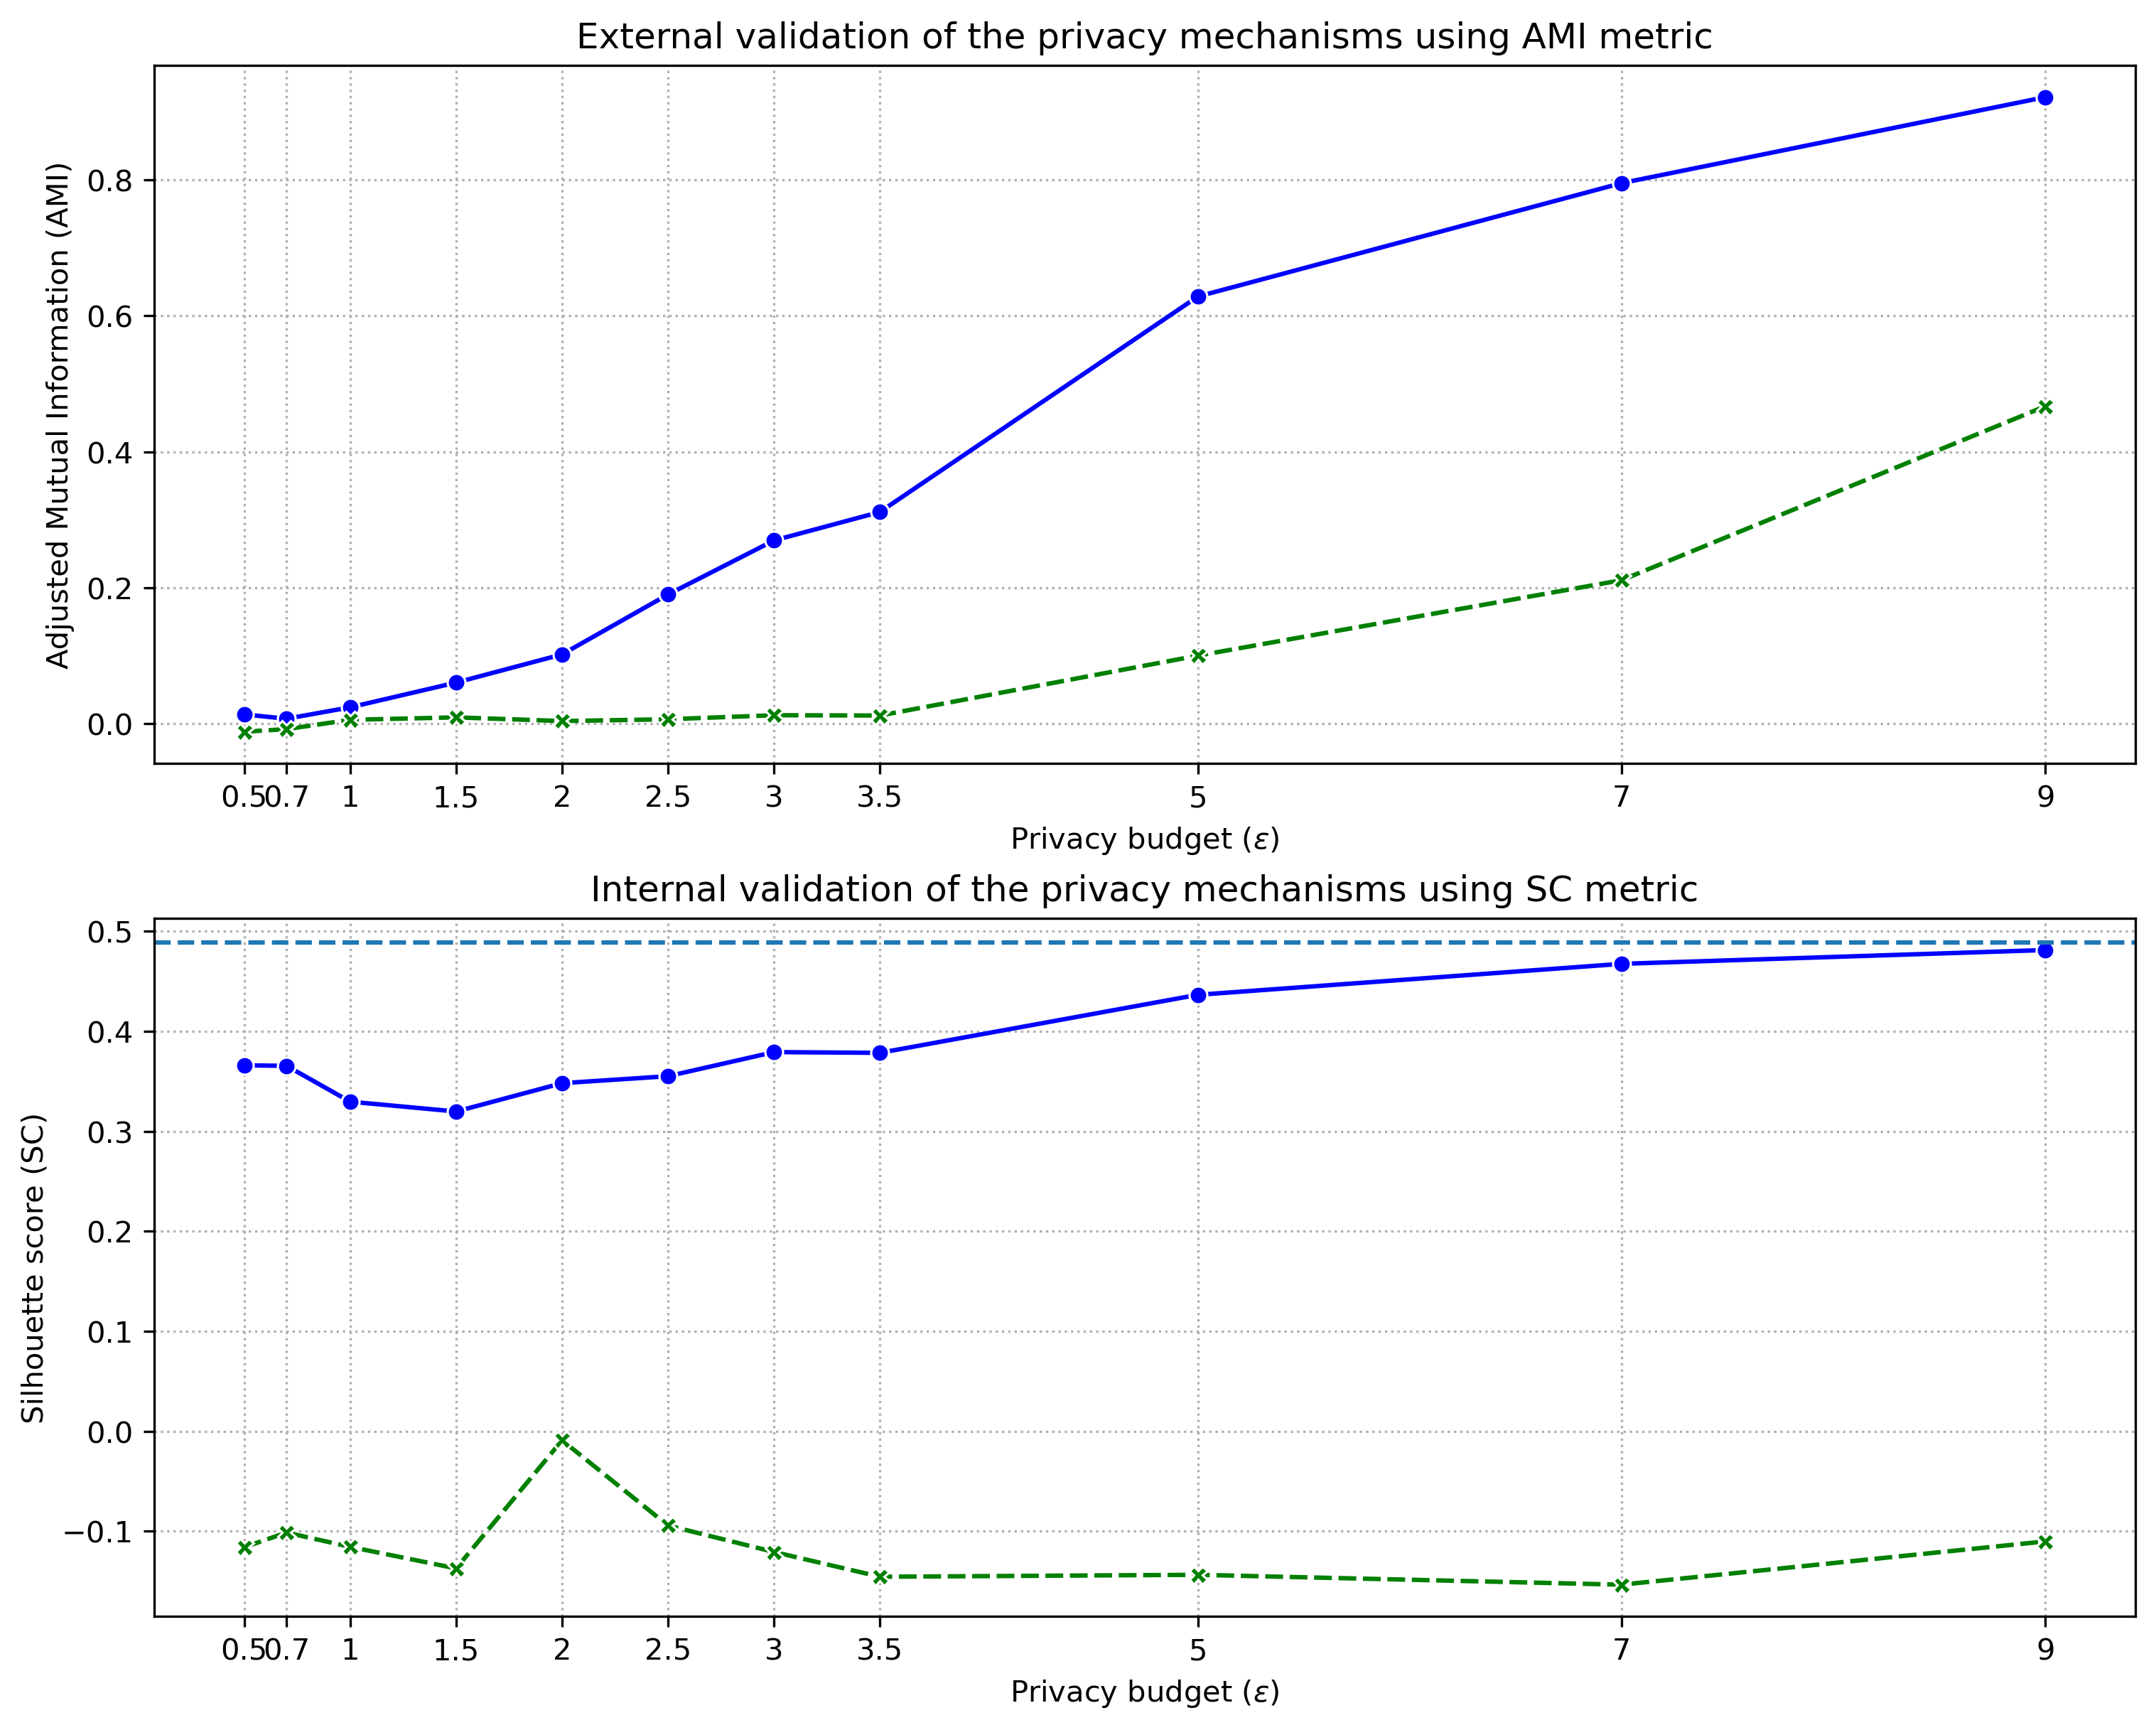
\includegraphics[width=0.65\textwidth]{Results/kd-laplace/piecewise/line-dataset/ami-and-sc_2_dimensions.png}
      \end{subfigure}
      \label{fig:validation-line-dataset_comparison_2d-laplace}
\end{figure}
The kD-Laplace algorithm performs best with a privacy budget of 5 for K-Means (\gls{ami} 0.55 - 0.6).
\gls{ag} performs slightly better with a budget of 9 (\gls{ami} 0.63).
Piecewise outperforms other methods, scoring 0.83 \gls{ami} for K-Means at budget 9 and better for different budgets, except for \gls{ag}.
For \gls{sc}, the mechanisms have similar scores, with Piecewise at baseline from budget 5, kD-Laplace at 7, and \gls{ag} beyond baseline from budget 9.

\newpage
\begin{figure}[H]
      \centering
      \begin{subfigure}{0.3\textwidth}
            \includegraphics[width=\textwidth]{Results/kd-laplace/kd-Laplace/skewed-dataset/legend_2.png}
      \end{subfigure}
      \begin{subfigure}{1\textwidth}
            \centering
            \caption{\textbf{AMI (top) and SC (bottom) for the kD-Laplace mechanism for the 2-dimensional data skewed-dataset}}
            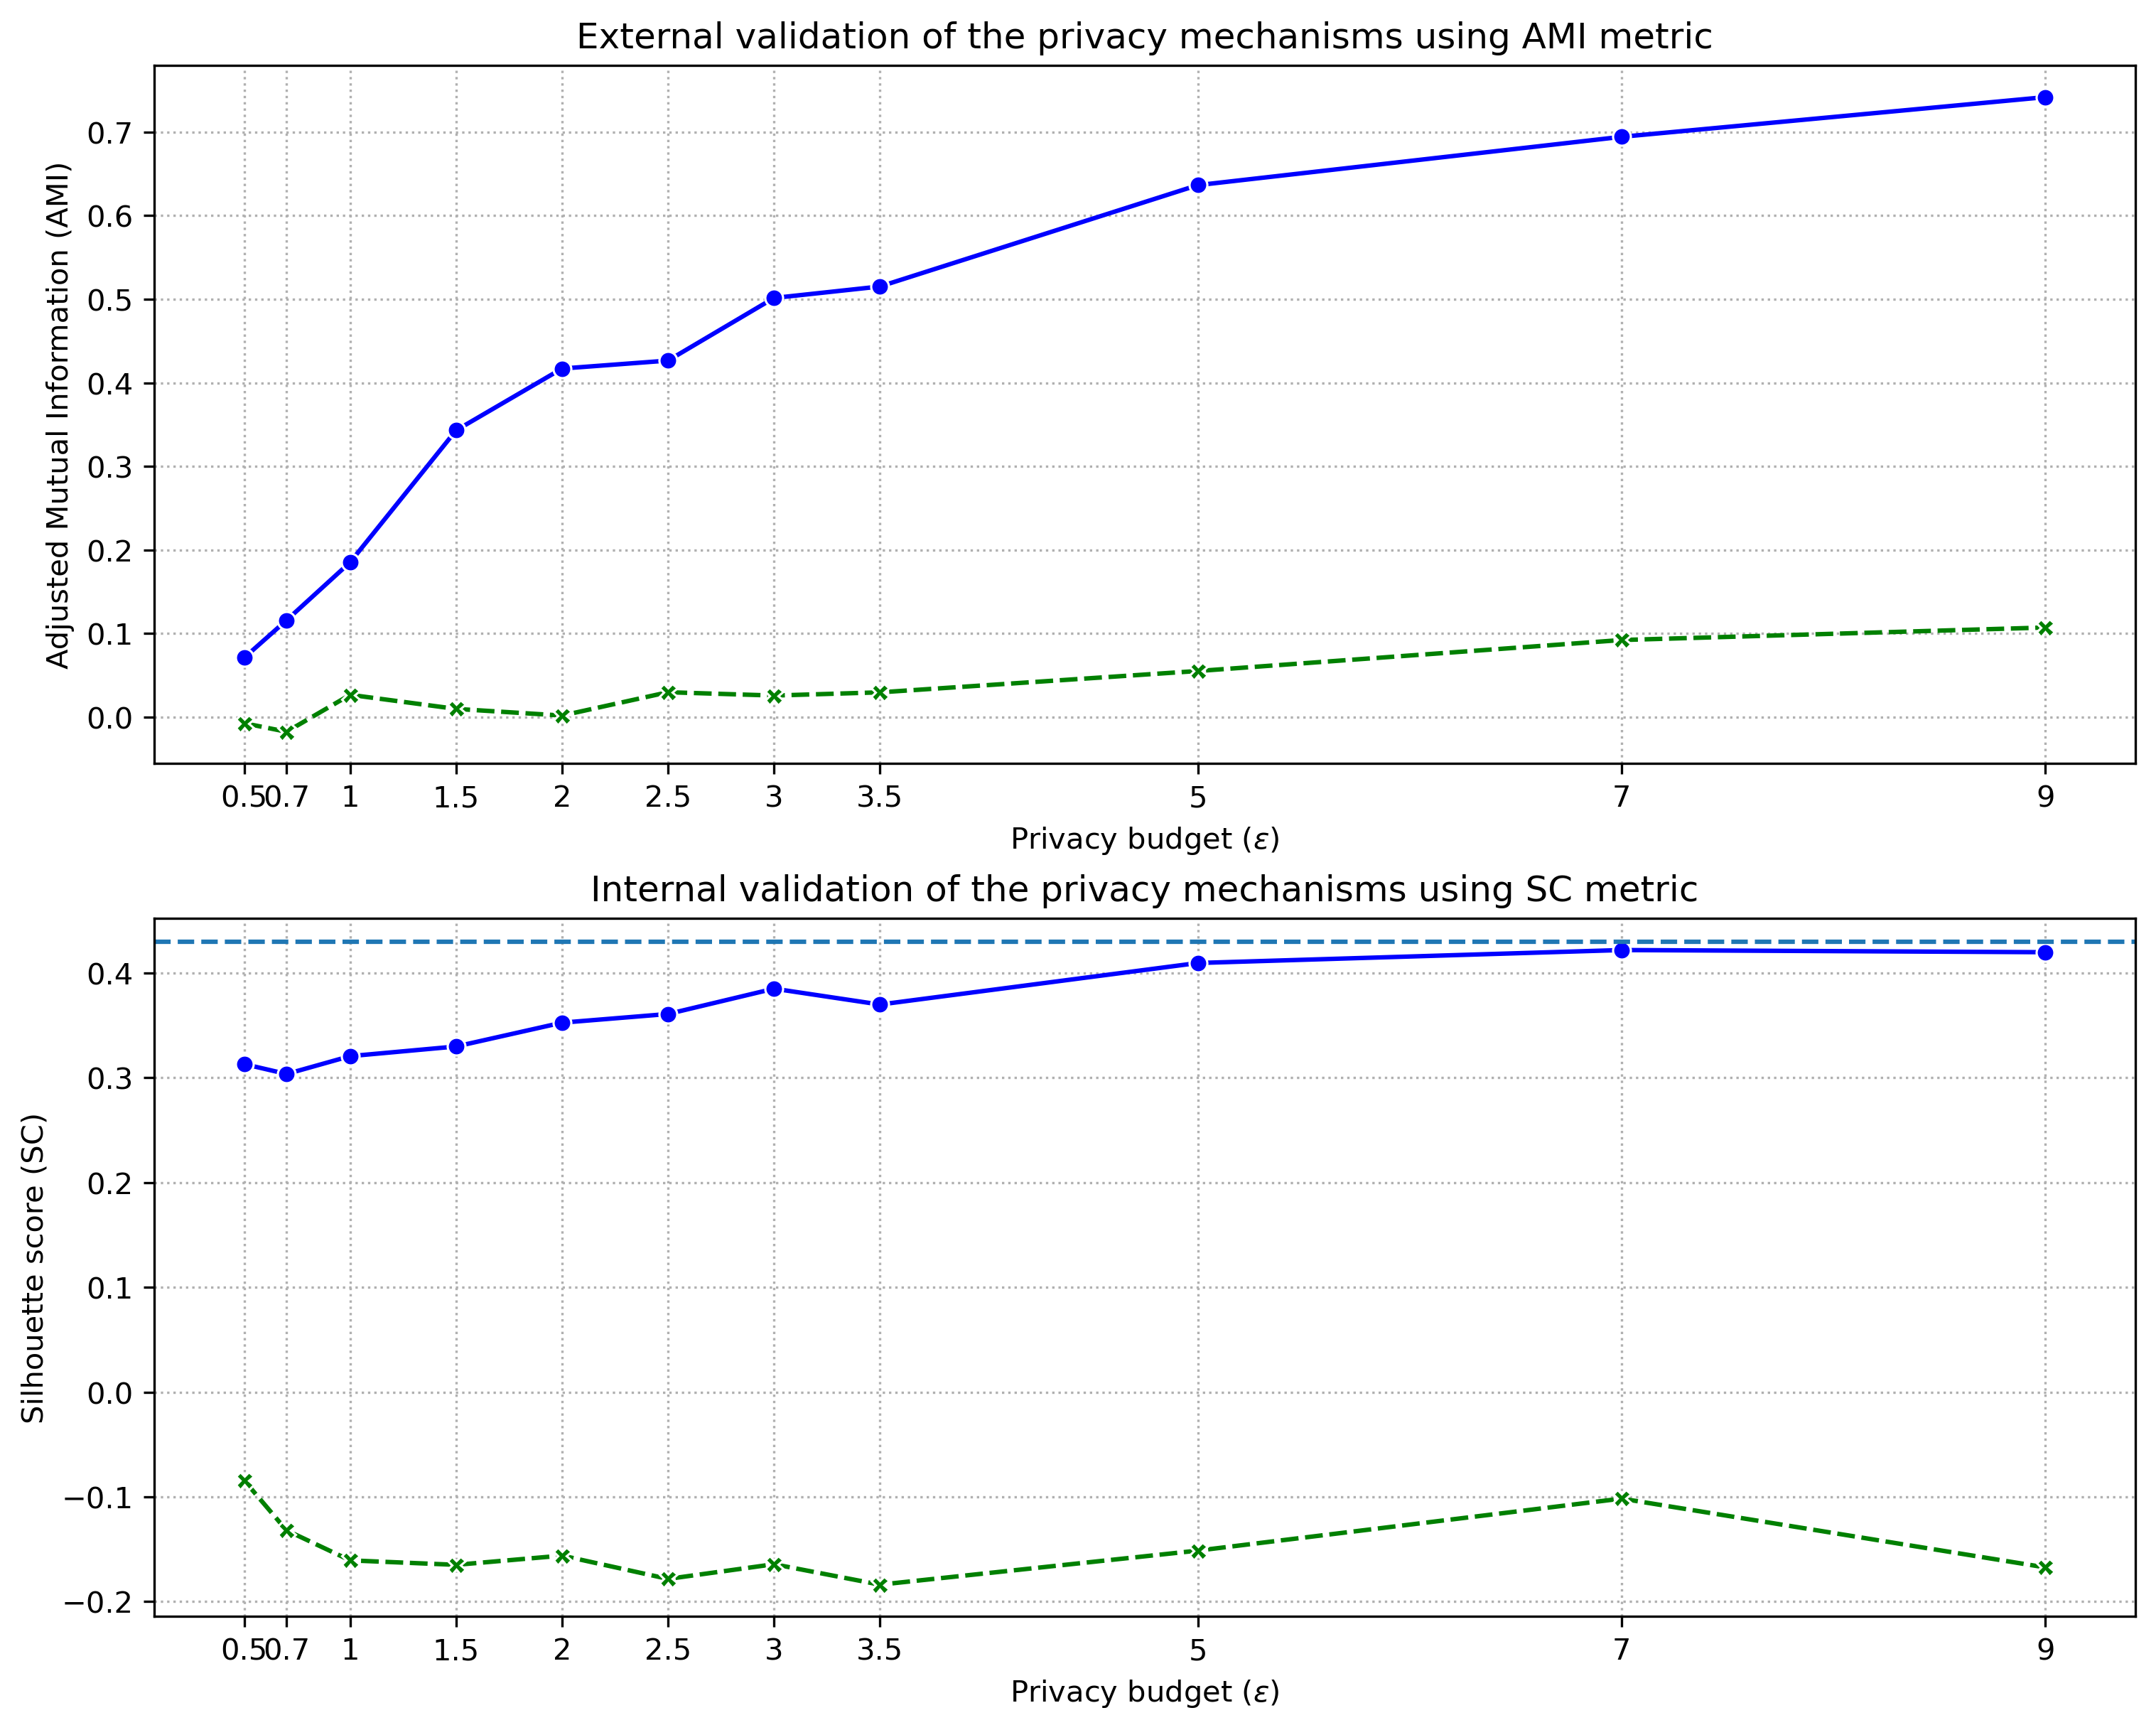
\includegraphics[width=0.65\textwidth]{Results/kd-laplace/kd-Laplace/skewed-dataset/ami-and-sc_2_dimensions.png}
            \centering
      \end{subfigure}
      \begin{subfigure}{1\textwidth}
            \centering
            \caption{\textbf{AMI (top) and SC (bottom) for the Piecewise mechanism for the 2-dimensional data skewed-dataset}}
            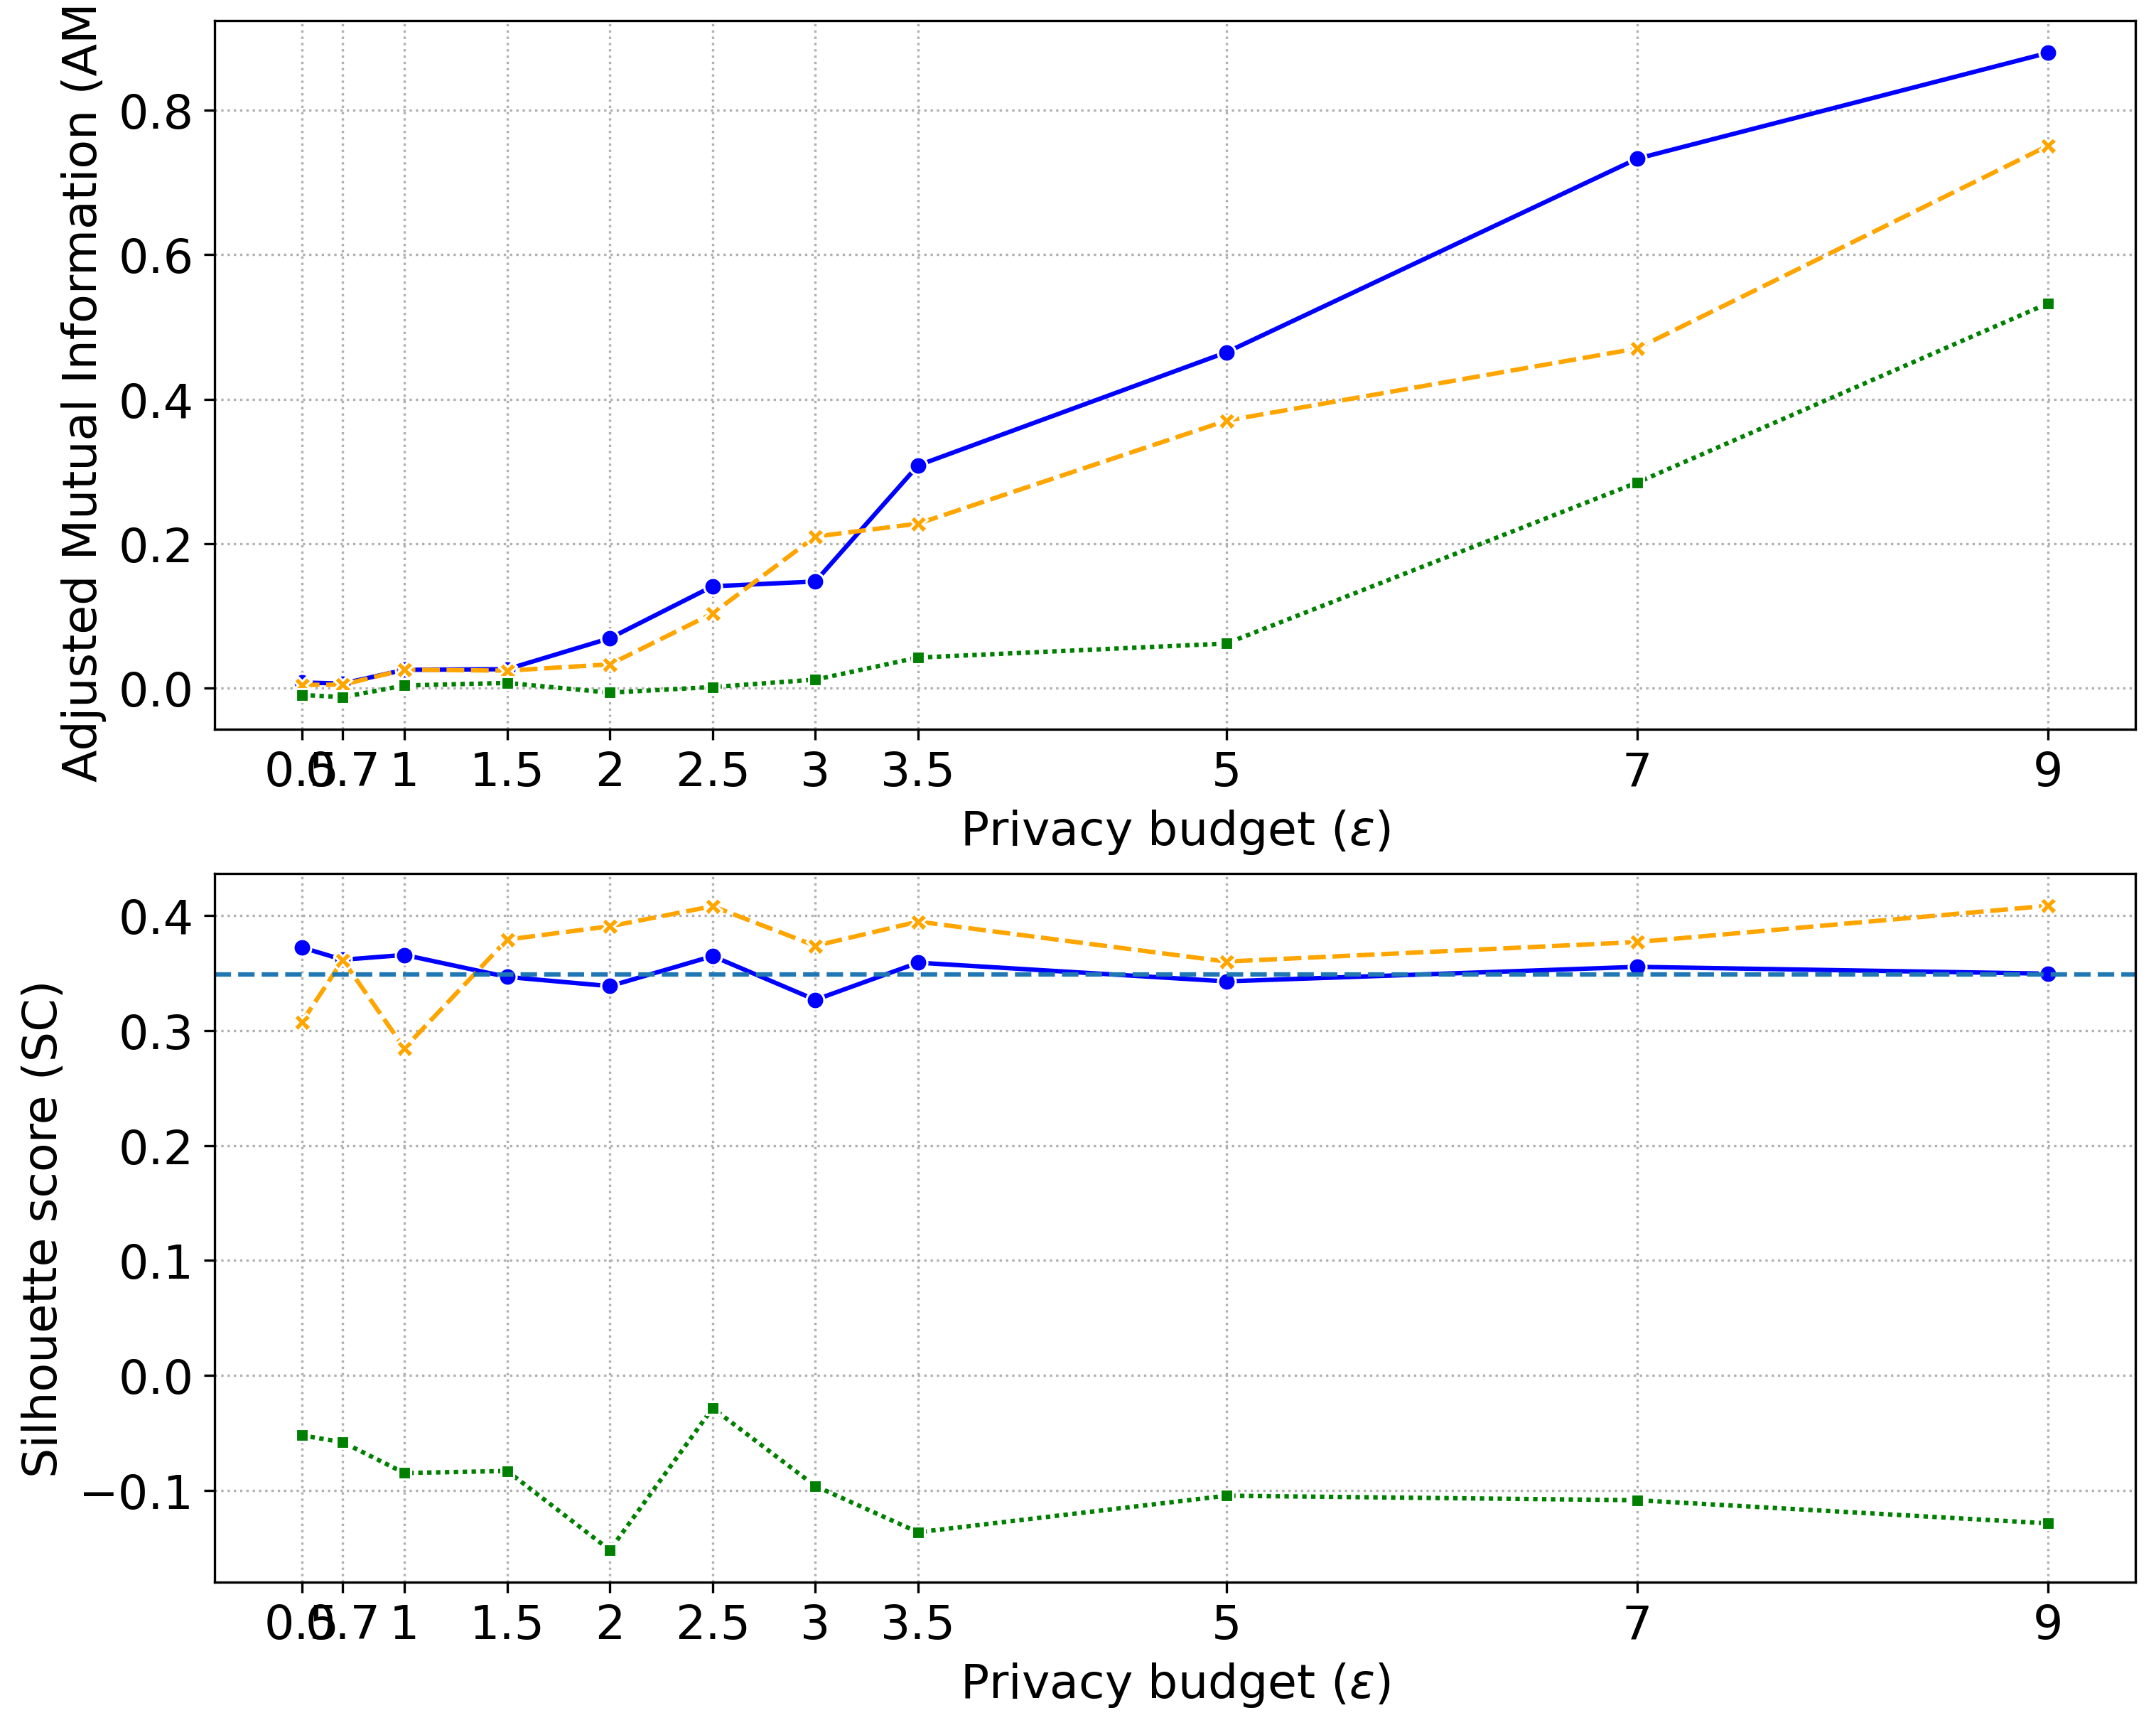
\includegraphics[width=0.65\textwidth]{Results/kd-laplace/piecewise/skewed-dataset/ami-and-sc_2_dimensions.png}
      \end{subfigure}
      \label{fig:validation-skewed-dataset_comparison_2d-laplace}
\end{figure}
kD-Laplace performs best with K-Means, reaching 0.63 \gls{ami} at privacy budget 9.
\gls{ag} follows, scoring 0.38 \gls{ami} at budgets 7 and 9.
Piecewise outperforms kD-Laplace for all clustering algorithms, scoring 0.82 \gls{ami} for K-Means at budget 9.
In terms of \gls{sc}, Piecewise also outperforms both K-Means and \gls{ag}, scoring above the baseline (0.4), while kD-Laplace is slightly worse (around 0.3).
\newpage
\subsection{3-dimensional data}
\begin{figure}[H]
      \centering
      \begin{subfigure}{0.30\textwidth}
            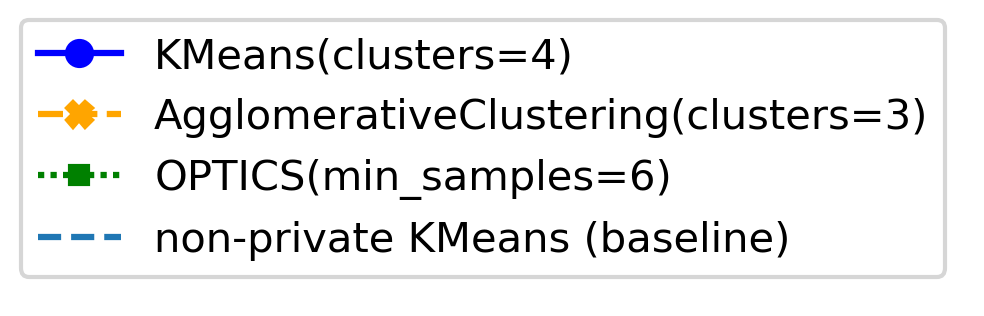
\includegraphics[width=\textwidth]{Results/kd-laplace/kd-Laplace/seeds-dataset/legend_3.png}
      \end{subfigure}
      \begin{subfigure}{1\textwidth}
            \caption{\textbf{AMI (top) and SC (bottom) for the kD-Laplace mechanism for the 3-dimensional data seeds-dataset}}
            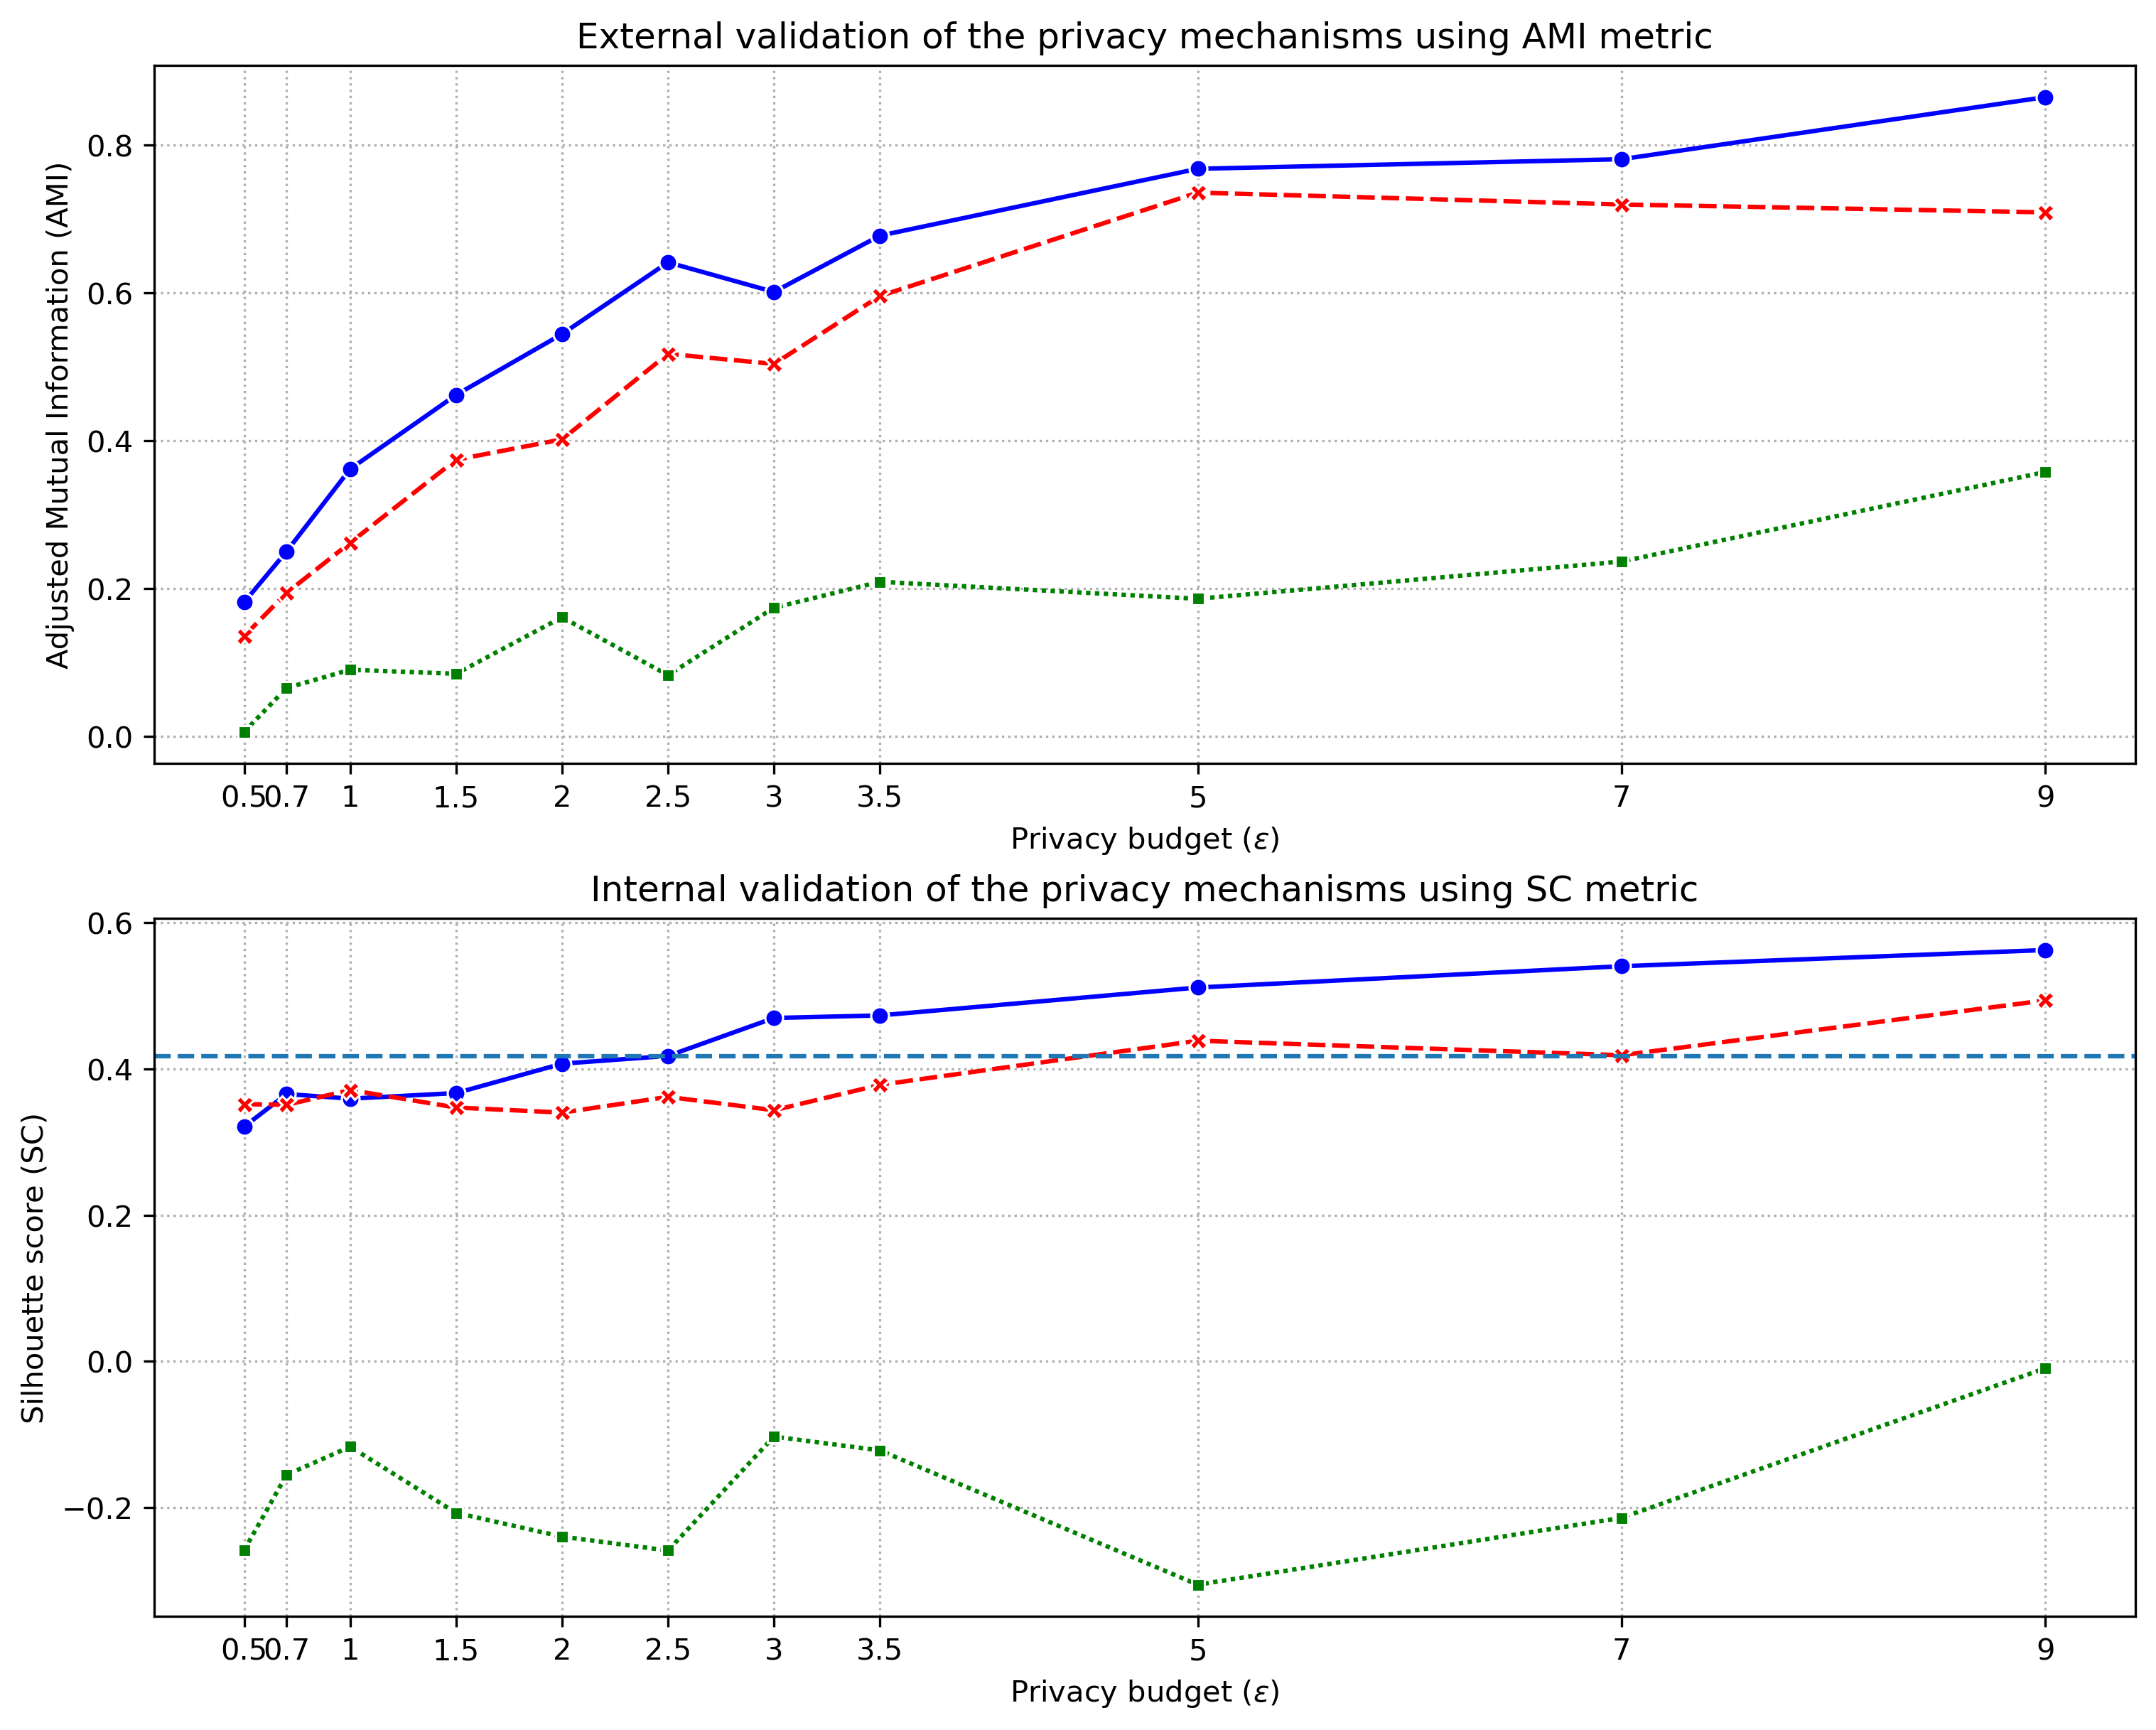
\includegraphics[width=0.65\textwidth]{Results/kd-laplace/kd-Laplace/seeds-dataset/ami-and-sc_3_dimensions.png}
            \centering
      \end{subfigure}
      \begin{subfigure}{1\textwidth}
            \caption{\textbf{AMI (top) and SC (bottom) for the Piecewise mechanism for the 3-dimensional data seeds-dataset}}
            \centering
            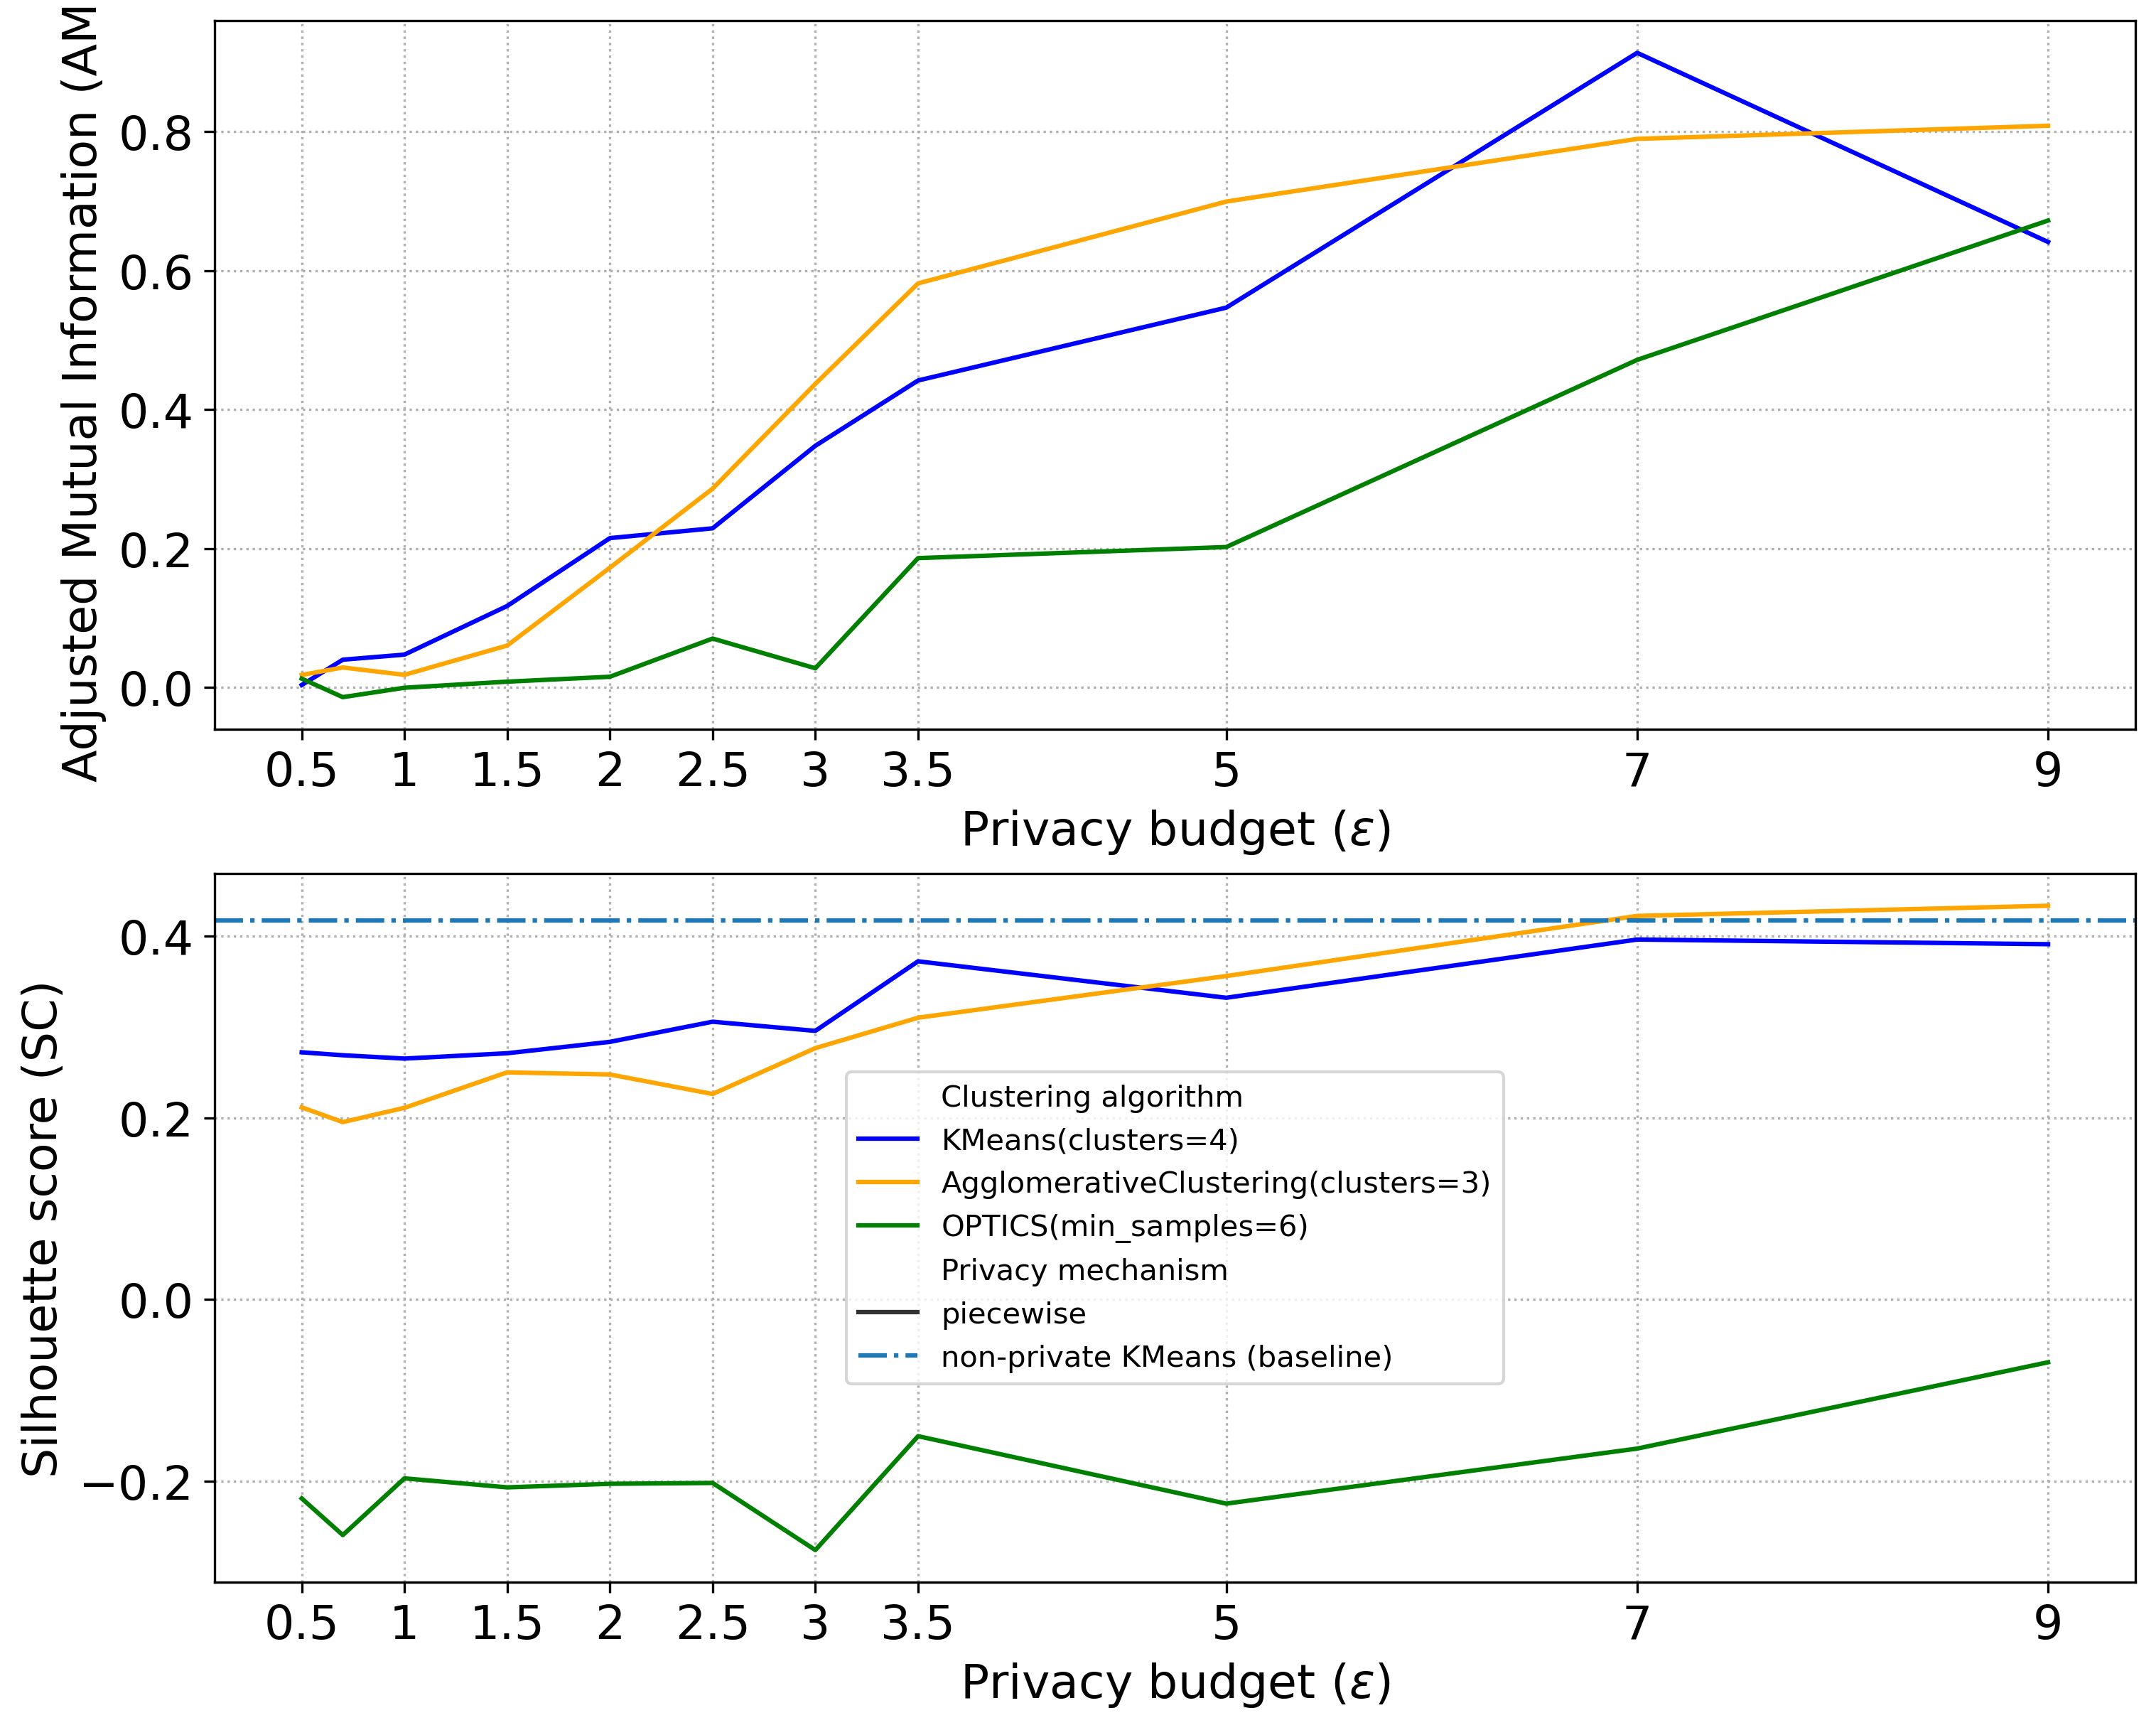
\includegraphics[width=0.65\textwidth]{Results/kd-laplace/piecewise/seeds-dataset/ami-and-sc_3_dimensions.png}
      \end{subfigure}
      \label{fig:validation-seeds-dataset_comparison_3d-laplace}
\end{figure}
Piecewise performs better for the \gls{ami} for privacy budgets 3.5 to 9 but worse for the lower epsilons (0.1 - 3.5).
K-Means scores 0.5 from epsilon 2 to 9 for kD-Laplace.
For both mechanisms, \gls{ag} scores the same as K-Means for both \gls{ami} and \gls{sc}.
\gls{optics} scores low (< 0.1) for kD-Laplace, but for Piecewise, it scores 0.4 and 0.6 for epsilon 7 and 9, respectively.
\newpage
\begin{figure}[H]
      \centering
      \begin{subfigure}{0.3\textwidth}
            \includegraphics[width=\textwidth]{Results/kd-laplace/kd-Laplace/heart-dataset/legend_3.png}
      \end{subfigure}
      \begin{subfigure}{1\textwidth}
            \caption{\textbf{AMI (top) and SC (bottom) for the kD-Laplace mechanism for the 3-dimensional data heart-dataset}}
            \centering
            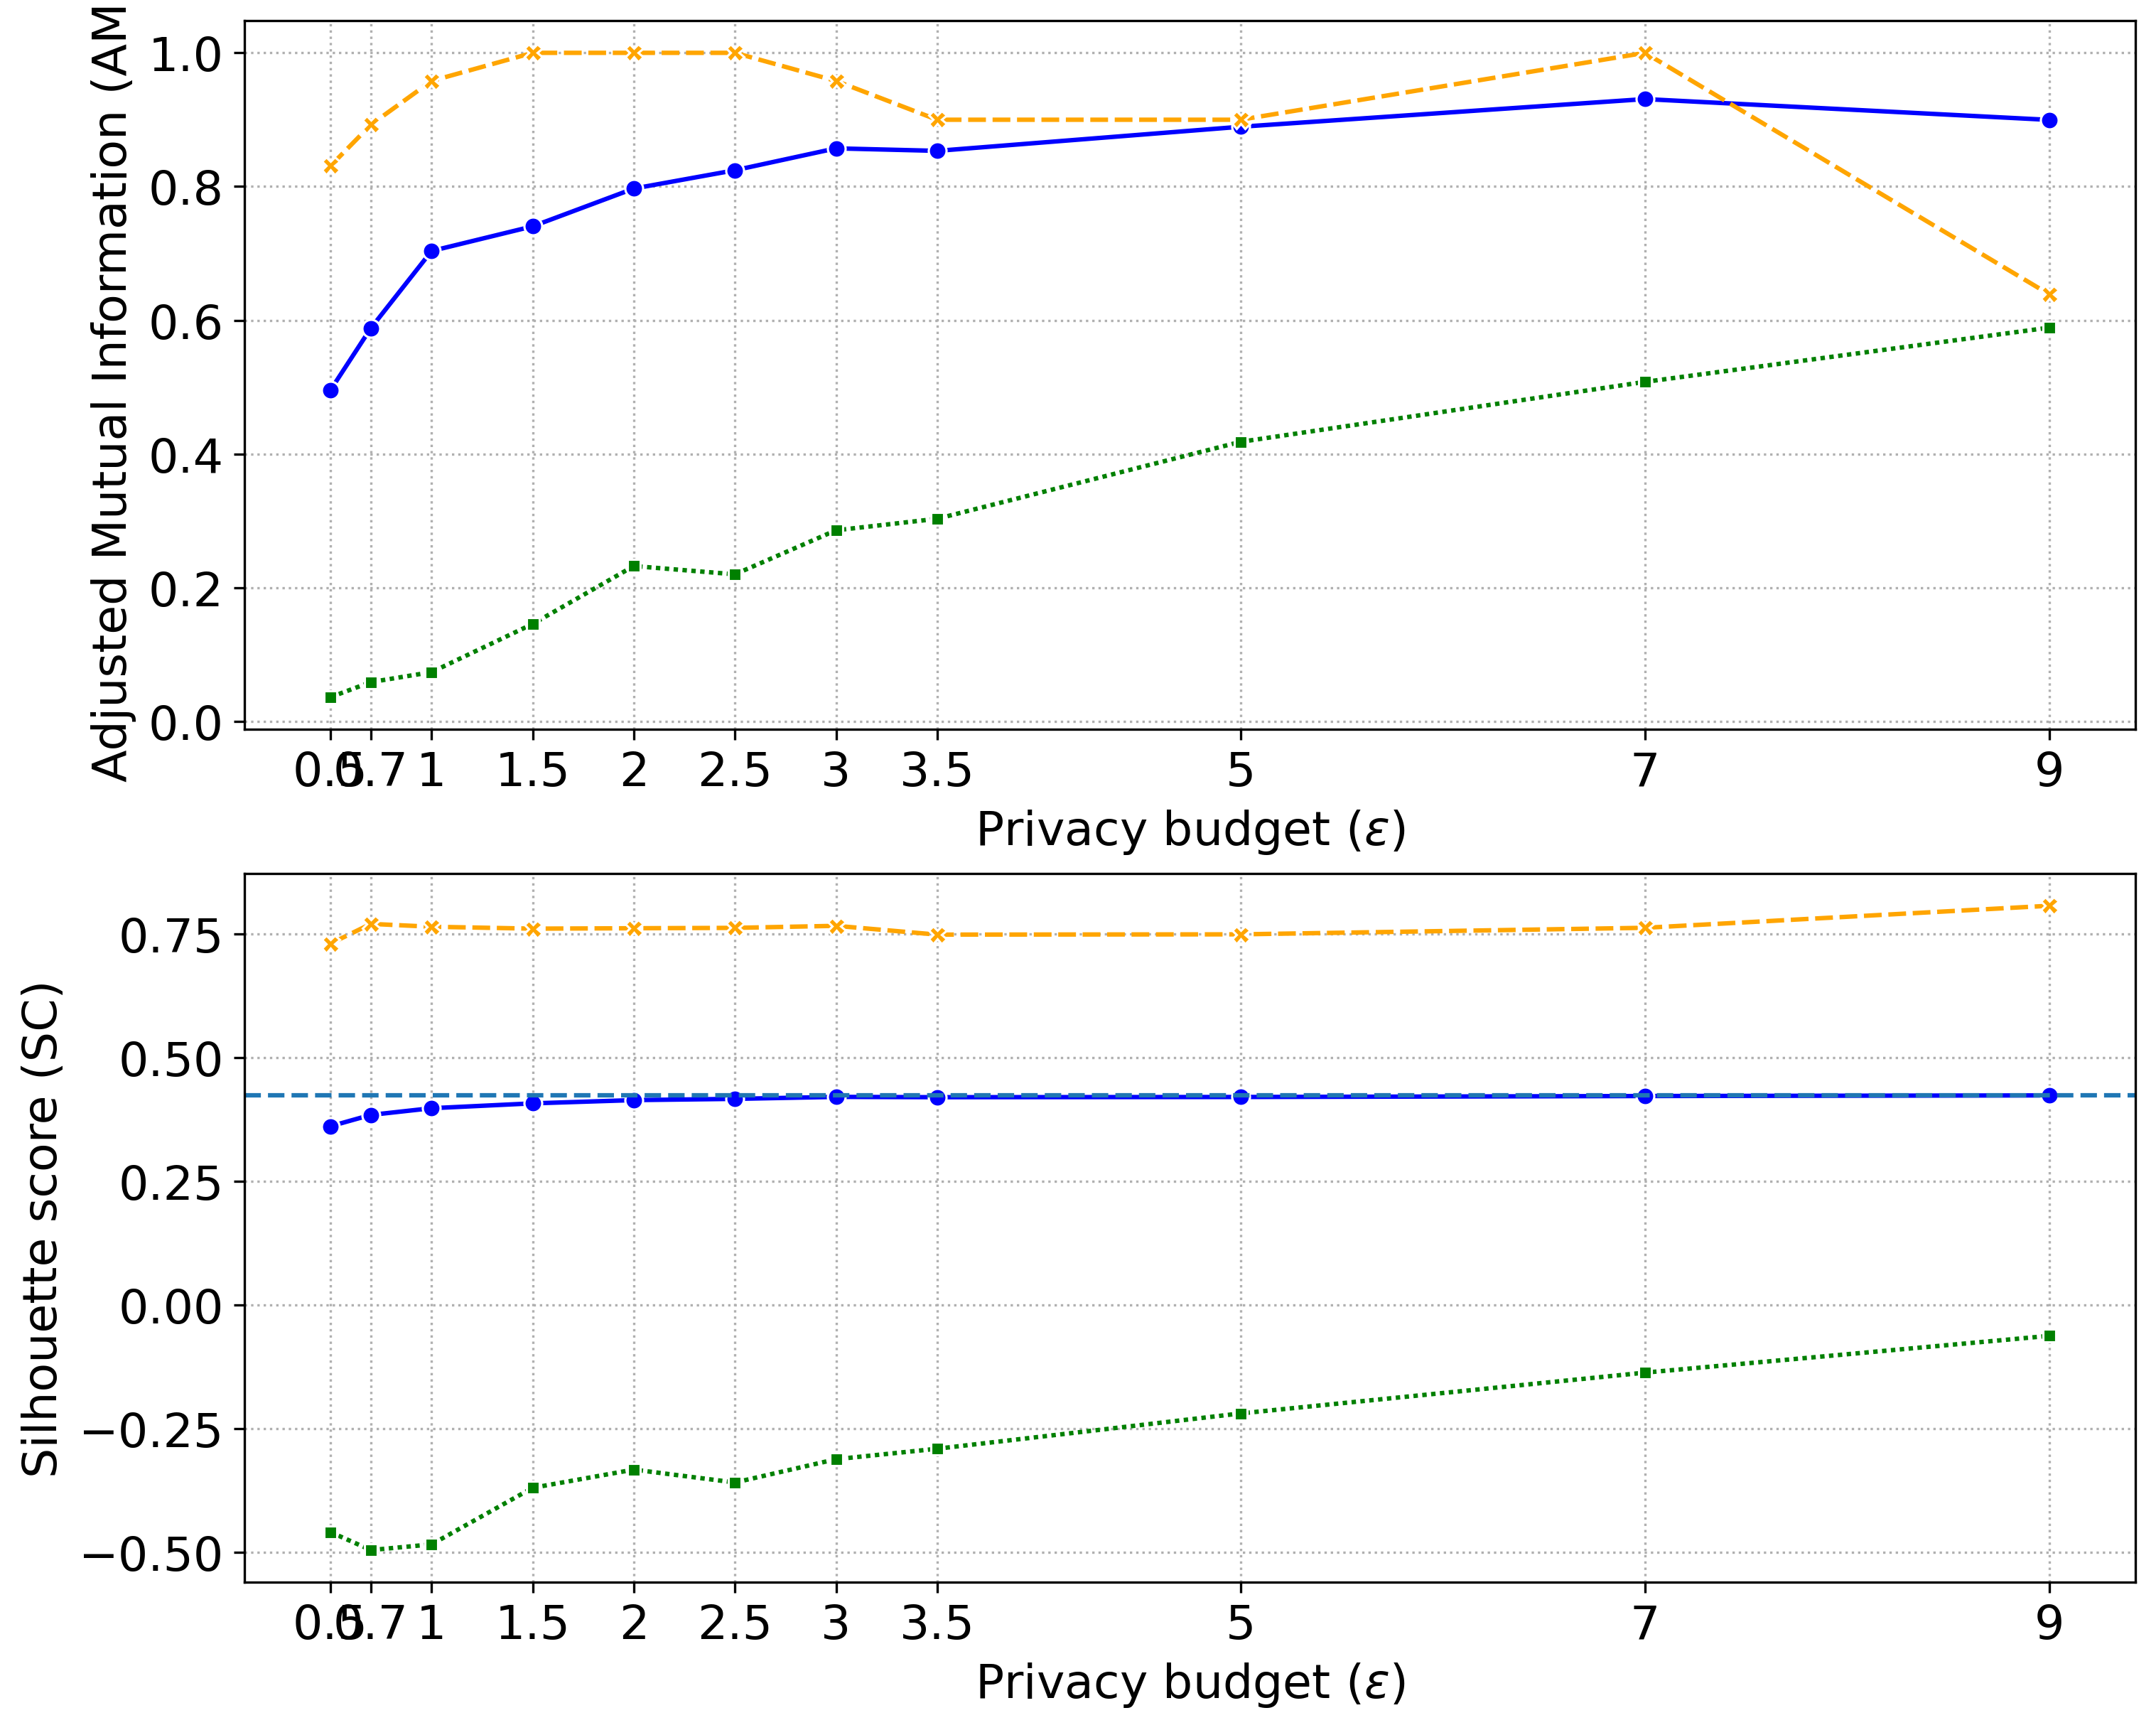
\includegraphics[width=0.65\textwidth]{Results/kd-laplace/kd-Laplace/heart-dataset/ami-and-sc_3_dimensions.png}
            \centering
      \end{subfigure}
      \begin{subfigure}{1\textwidth}
            \caption{\textbf{AMI (top) and SC (bottom) for the Piecewise mechanism for the 3-dimensional data heart-dataset}}
            \centering
            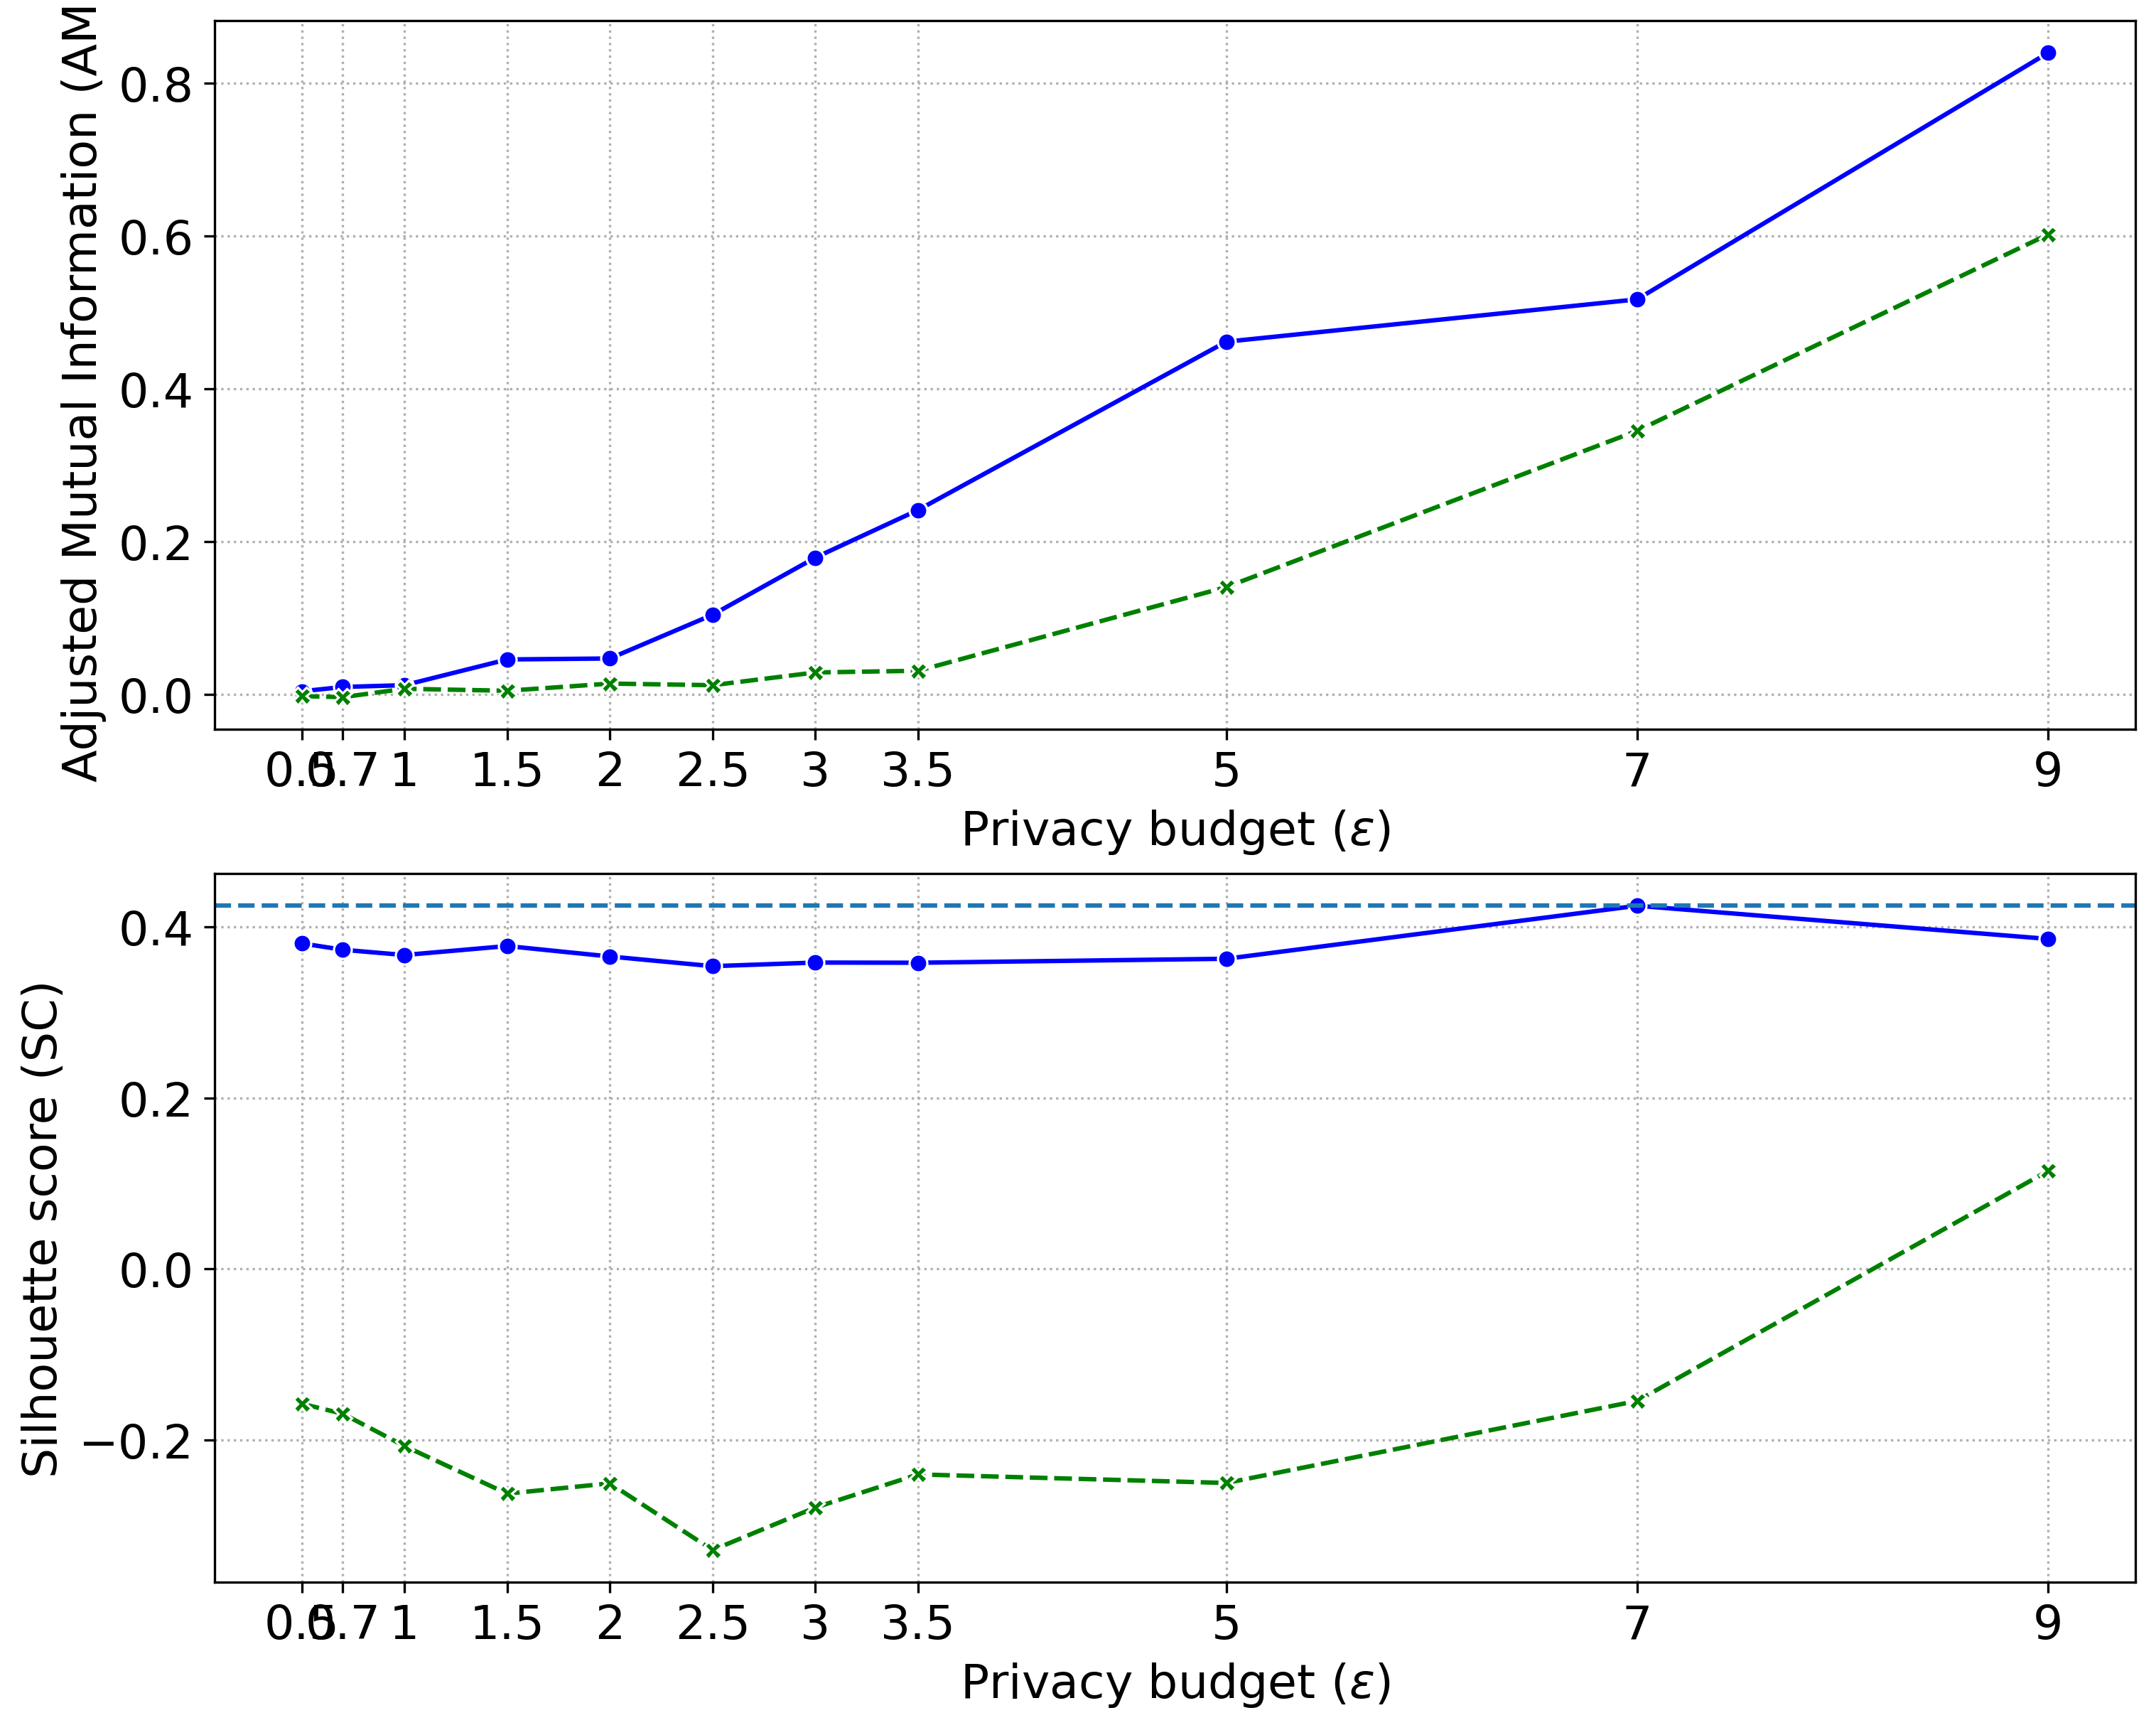
\includegraphics[width=0.65\textwidth]{Results/kd-laplace/piecewise/heart-dataset/ami-and-sc_3_dimensions.png}
      \end{subfigure}
      \label{fig:validation-heart-dataset_comparison_3d-laplace}
\end{figure}
KD-Laplace performs well (+/- 0.90 \gls{ami}) for K-Means at budgets 7 and 9.
\gls{ag} scores around +/- 1.0 \gls{ami} for epsilon values of 1.5 to 2.5, staying above 0.8 for most budgets.
\gls{optics} scores better (0.6 \gls{ami} at budget 9).
Piecewise scores below 0.6 \gls{ami} for budgets < 7, reaching a maximum of 0.8 \gls{ami} for K-Means.
For \gls{sc}, both Piecewise and kD-Laplace reach the baseline for \gls{ag} and K-Means.
KD-Laplace surpasses the baseline by 0.25 for \gls{ag}.
\newpage
\begin{figure}[H]
      \centering
      \begin{subfigure}{0.3\textwidth}
            \includegraphics[width=\textwidth]{Results/kd-laplace/kd-Laplace/circle-dataset/legend_3.png}
      \end{subfigure}
      \begin{subfigure}{1\textwidth}
            \caption{\textbf{AMI (top) and SC (bottom) for the kD-Laplace mechanism for the 3-dimensional data circle-dataset}}
            \centering
            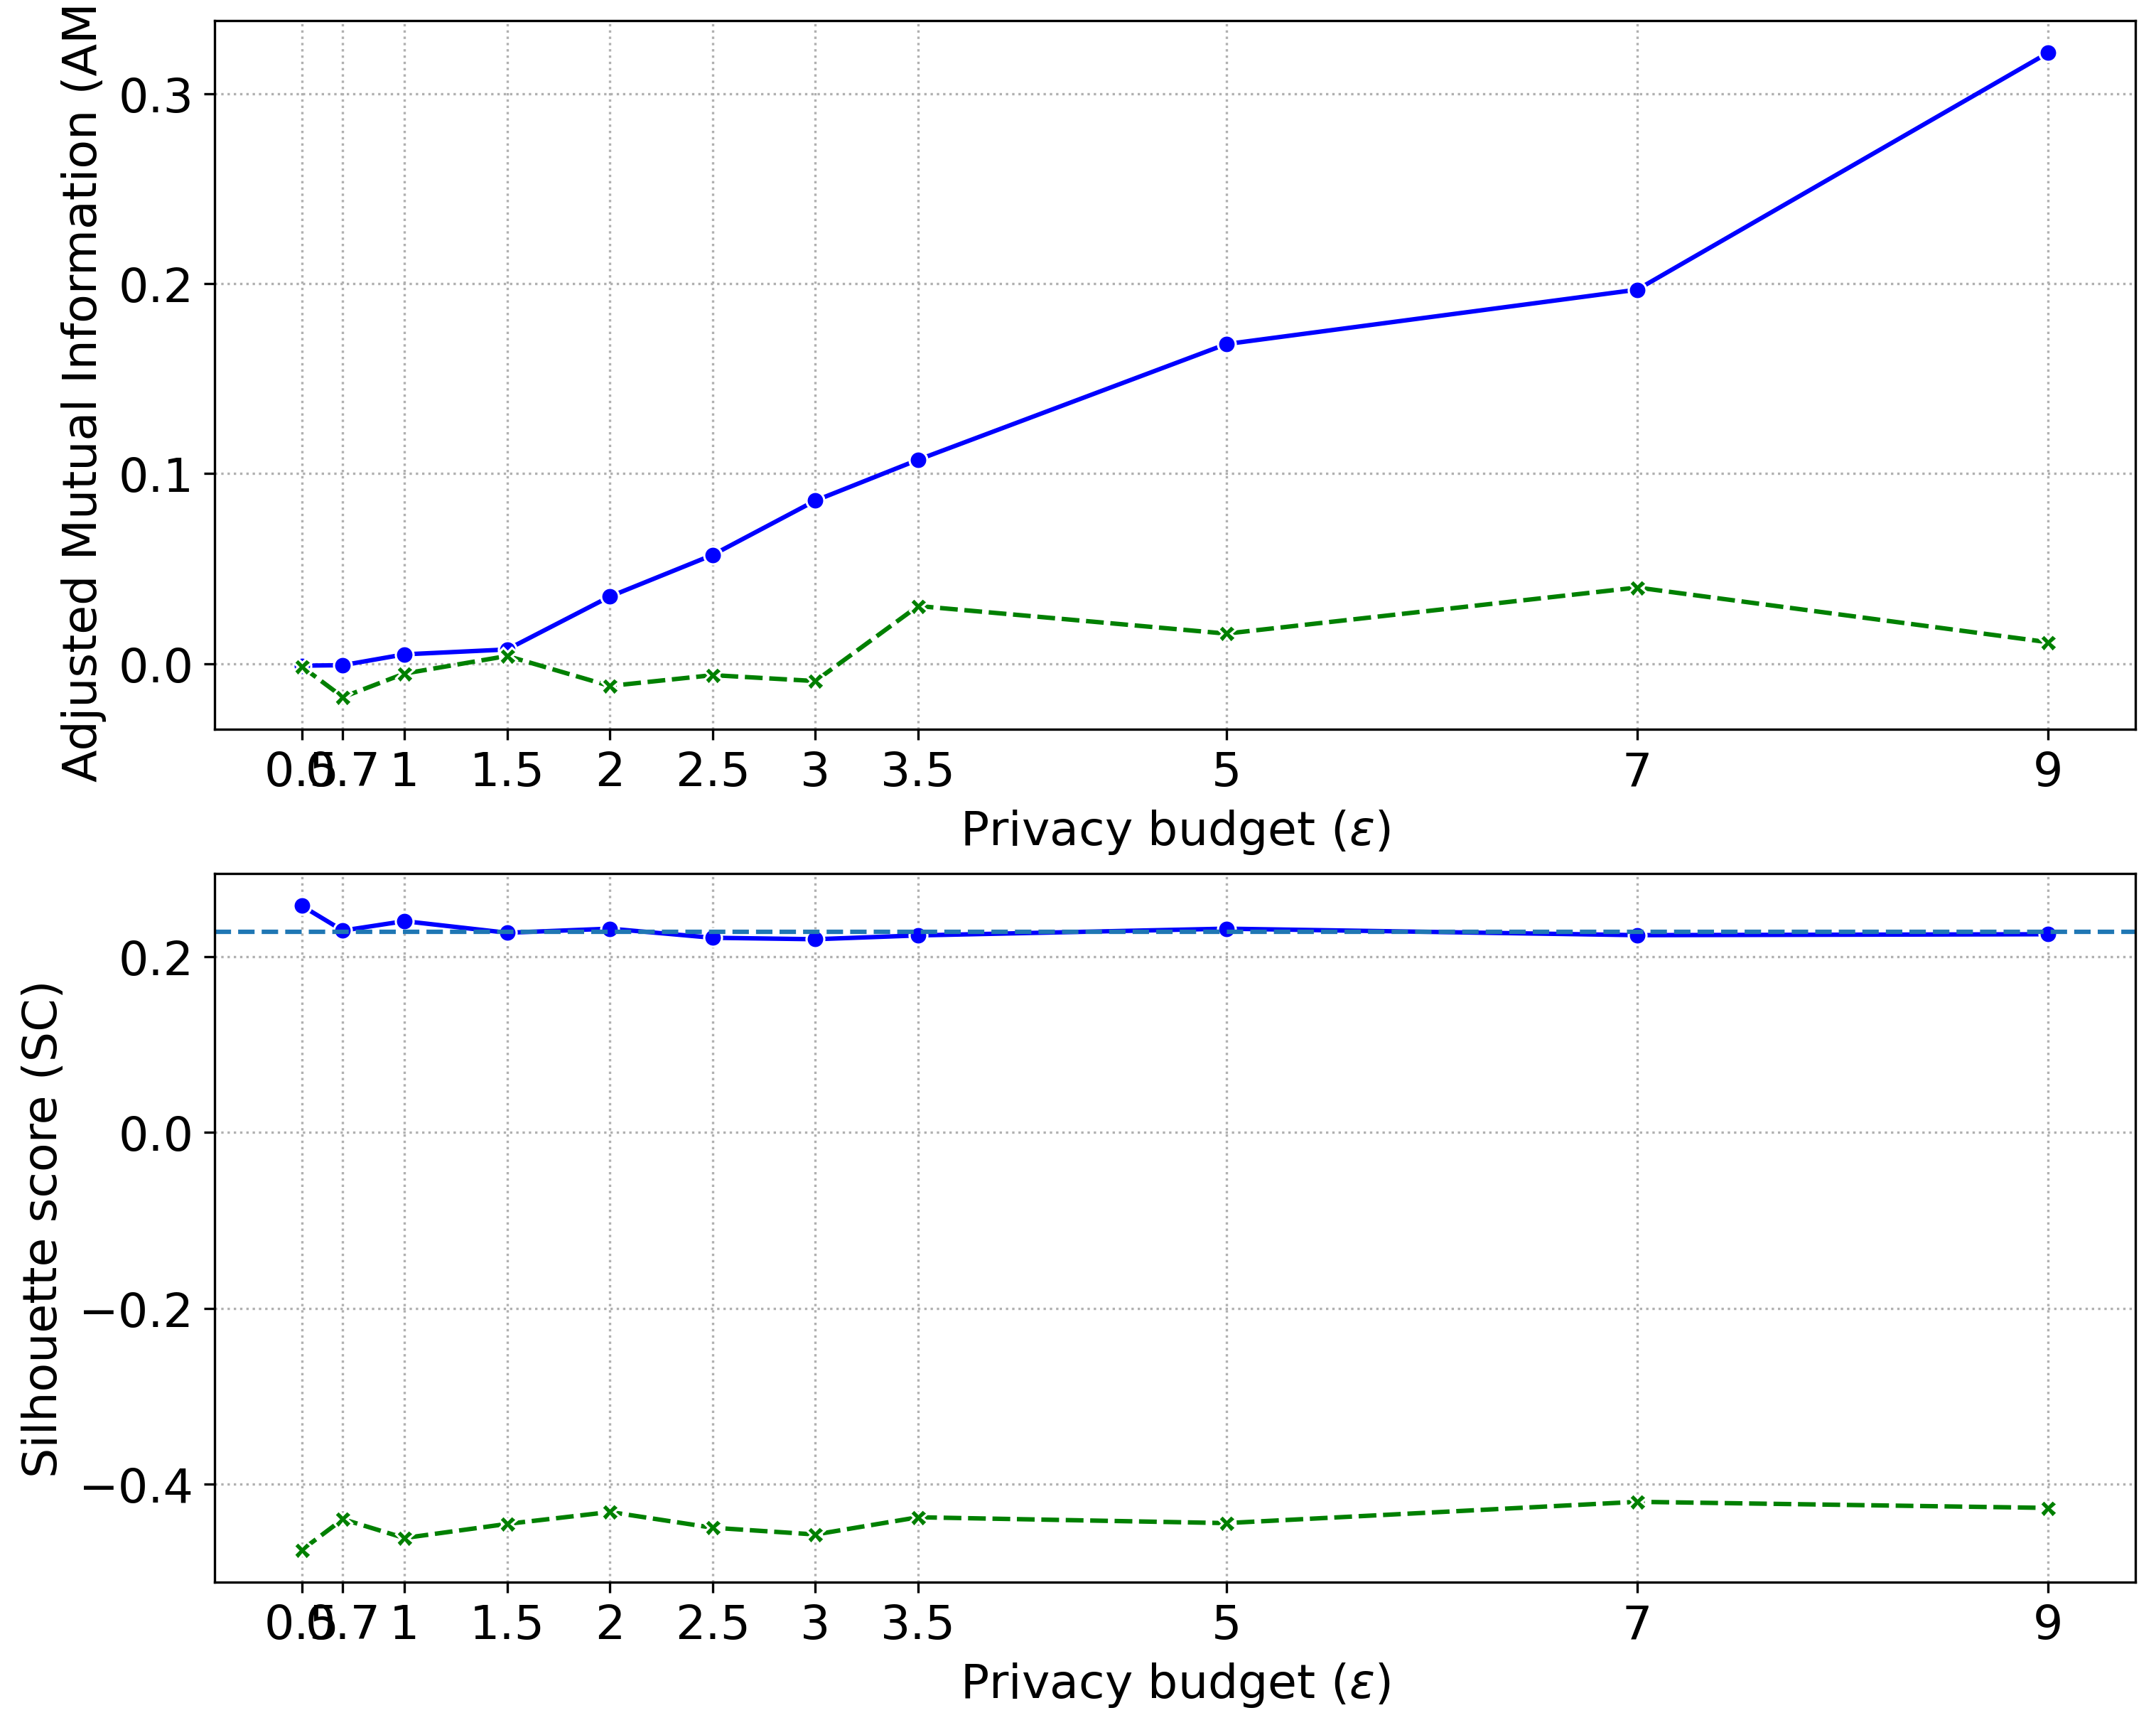
\includegraphics[width=0.65\textwidth]{Results/kd-laplace/kd-Laplace/circle-dataset/ami-and-sc_3_dimensions.png}
            \centering
      \end{subfigure}
      \begin{subfigure}{1\textwidth}
            \caption{\textbf{AMI (top) and SC (bottom) for the Piecewise mechanism for the 3-dimensional data circle-dataset}}
            \centering
            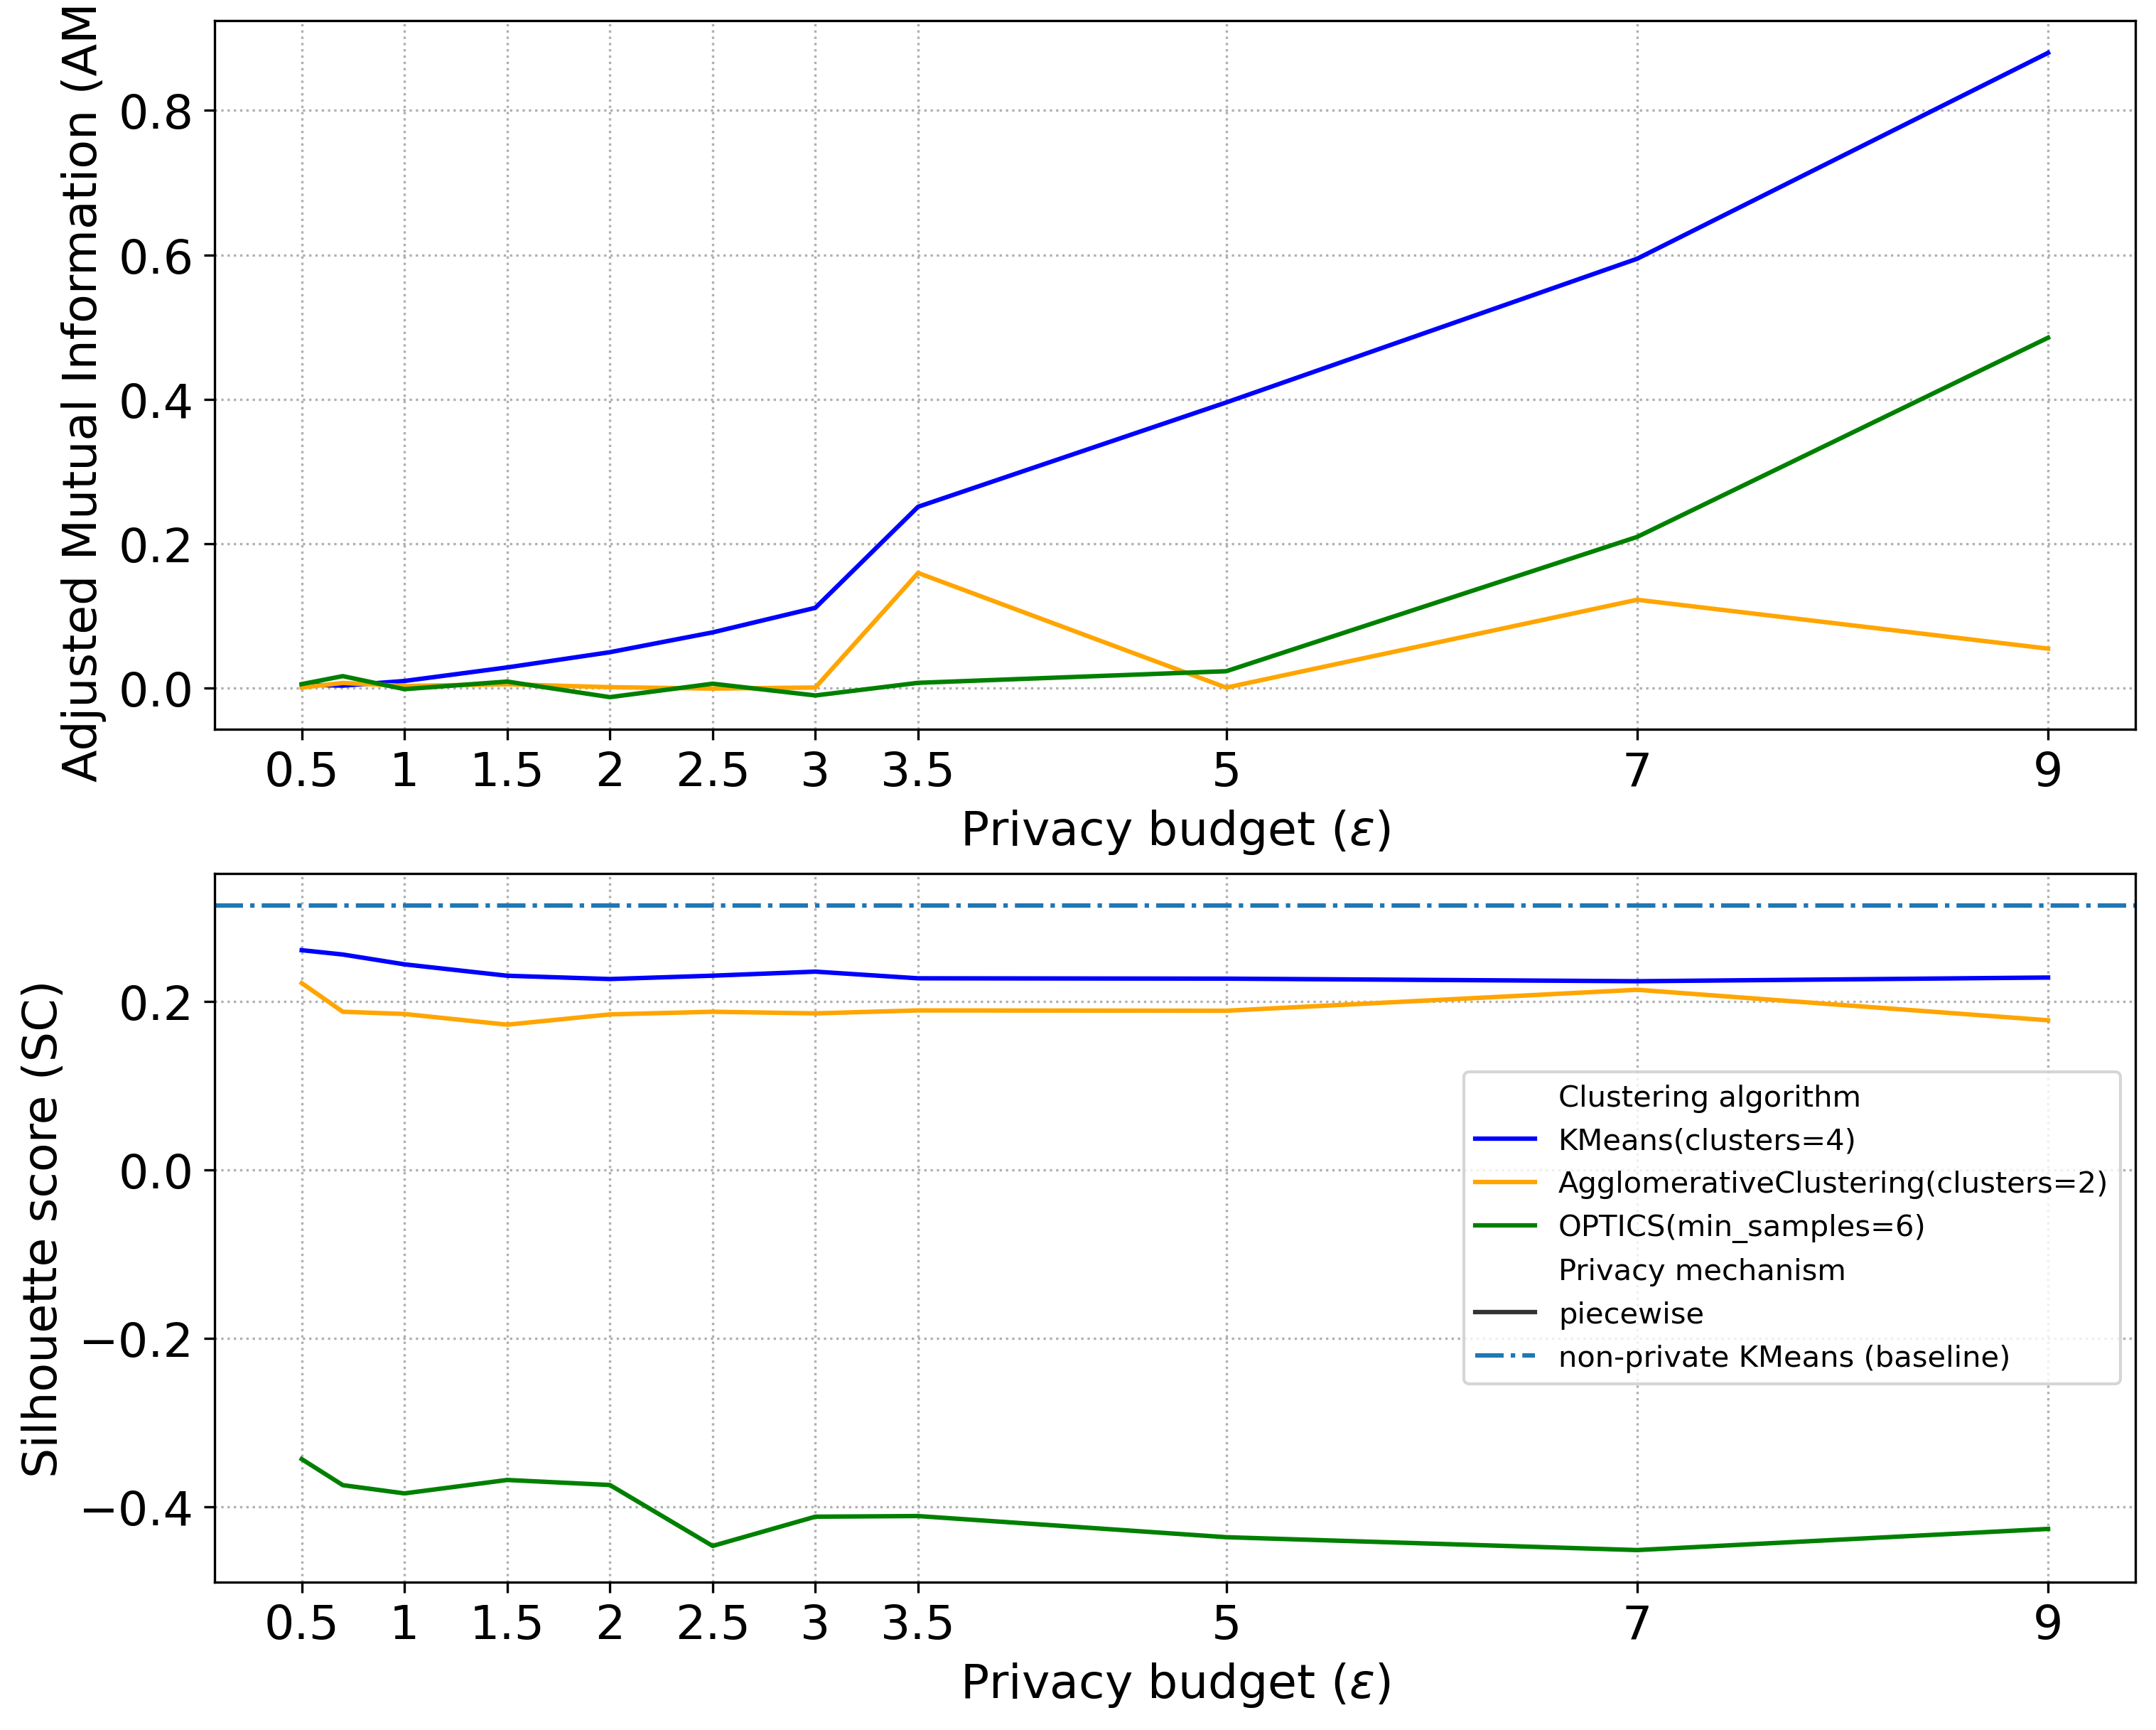
\includegraphics[width=0.65\textwidth]{Results/kd-laplace/piecewise/circle-dataset/ami-and-sc_3_dimensions.png}
      \end{subfigure}
      \label{fig:validation-circle-dataset_comparison_3d-laplace}
\end{figure}
kD-Laplace performs best with K-Means, scoring a maximum of 0.33 \gls{ami}. The other algorithms perform poorly (< 0.1 \gls{ami}).
Piecewise also shows the best results with K-Means, scoring 0.82 \gls{ami}, while the other algorithms perform weakly (< 0.2 \gls{ami}).
\gls{optics} performs relatively well with 0.49 \gls{ami} at privacy budget 9.
Both mechanisms have similar \gls{sc} scores (around 0.2), which is at the baseline level.
\gls{optics} performs below 0 \gls{sc} for all privacy budgets.
\newpage
\begin{figure}[H]
      \centering
      \begin{subfigure}{0.3\textwidth}
            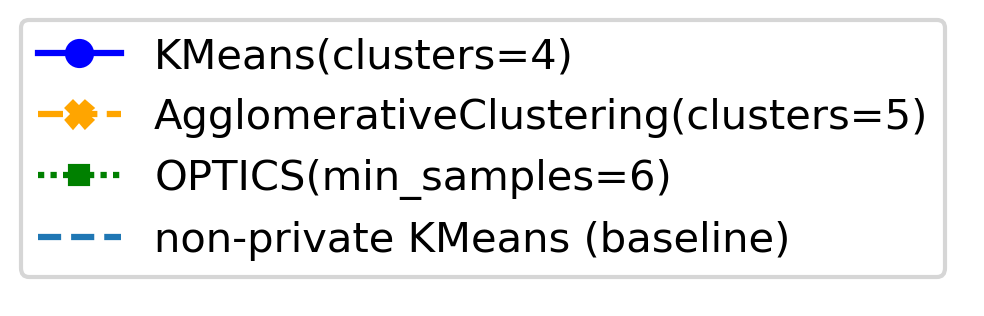
\includegraphics[width=\textwidth]{Results/kd-laplace/kd-Laplace/line-dataset/legend_3.png}
      \end{subfigure}
      \begin{subfigure}{1\textwidth}
            \caption{\textbf{AMI (top) and SC (bottom) for the kD-Laplace mechanism for the 3-dimensional data line-dataset}}
            \centering
            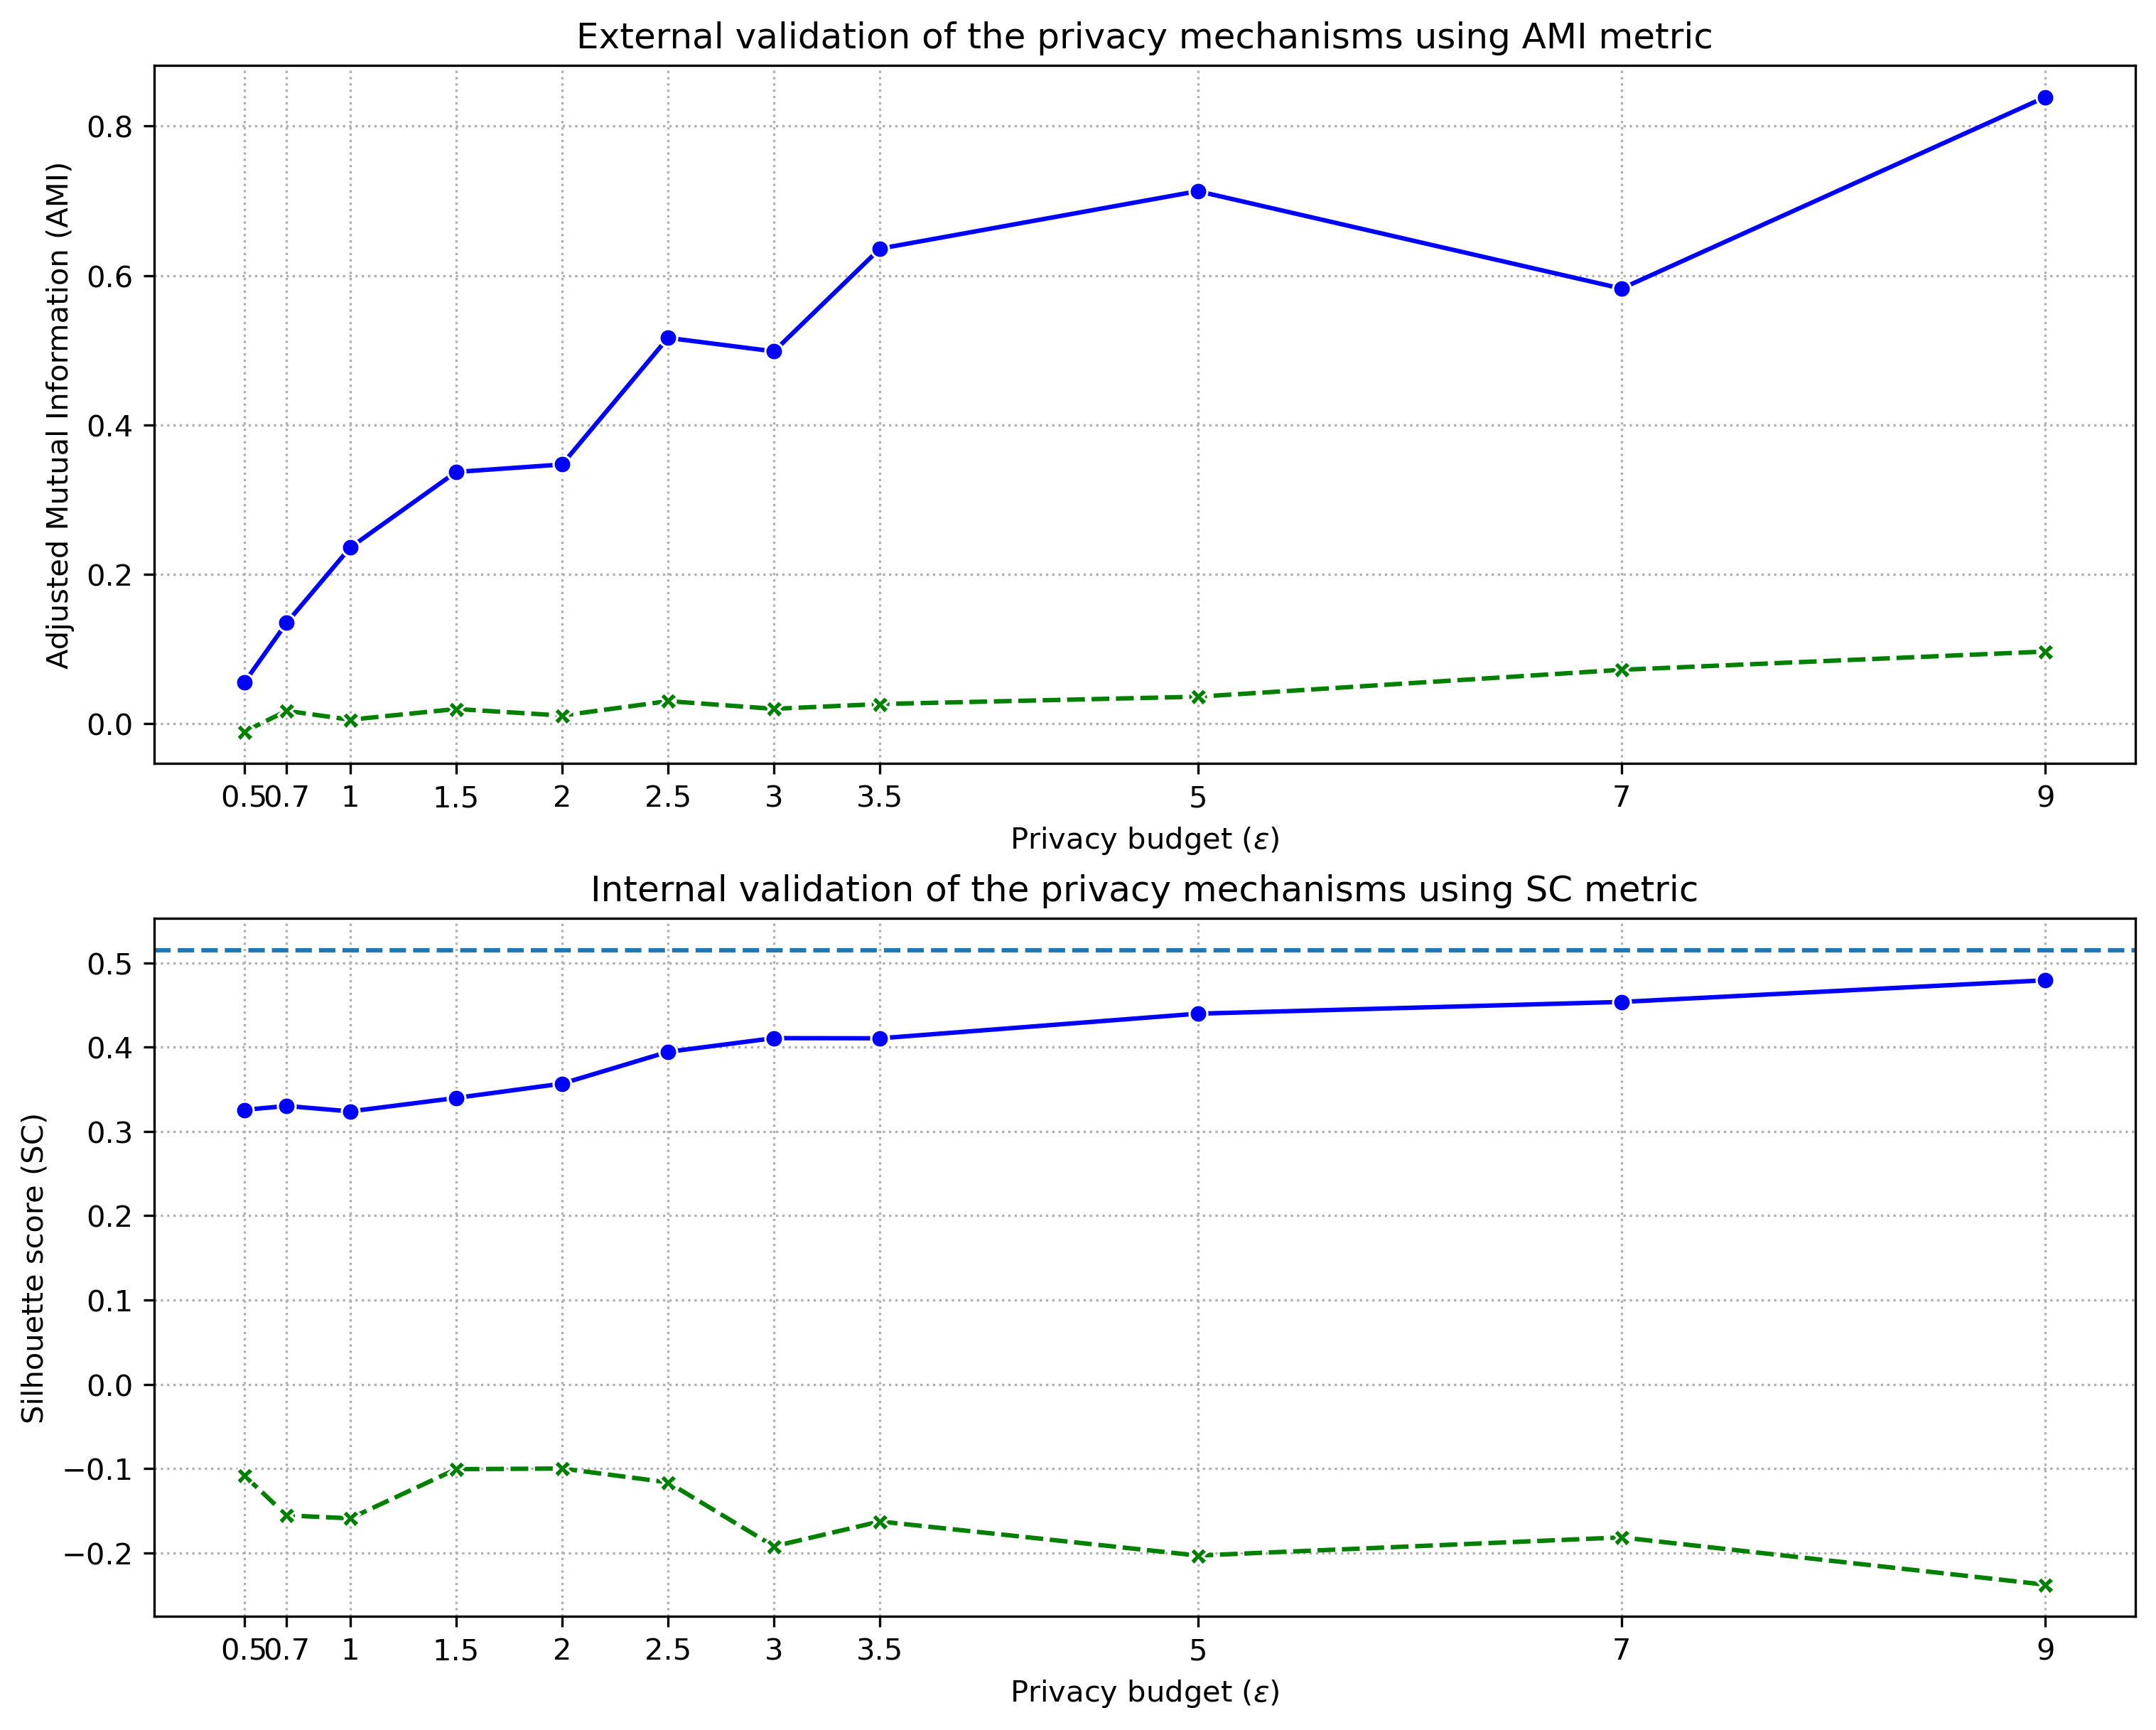
\includegraphics[width=0.65\textwidth]{Results/kd-laplace/kd-Laplace/line-dataset/ami-and-sc_3_dimensions.png}
            \centering
      \end{subfigure}
      \begin{subfigure}{1\textwidth}
            \caption{\textbf{AMI (top) and SC (bottom) for the Piecewise mechanism for the 3-dimensional data line-dataset}}
            \centering
            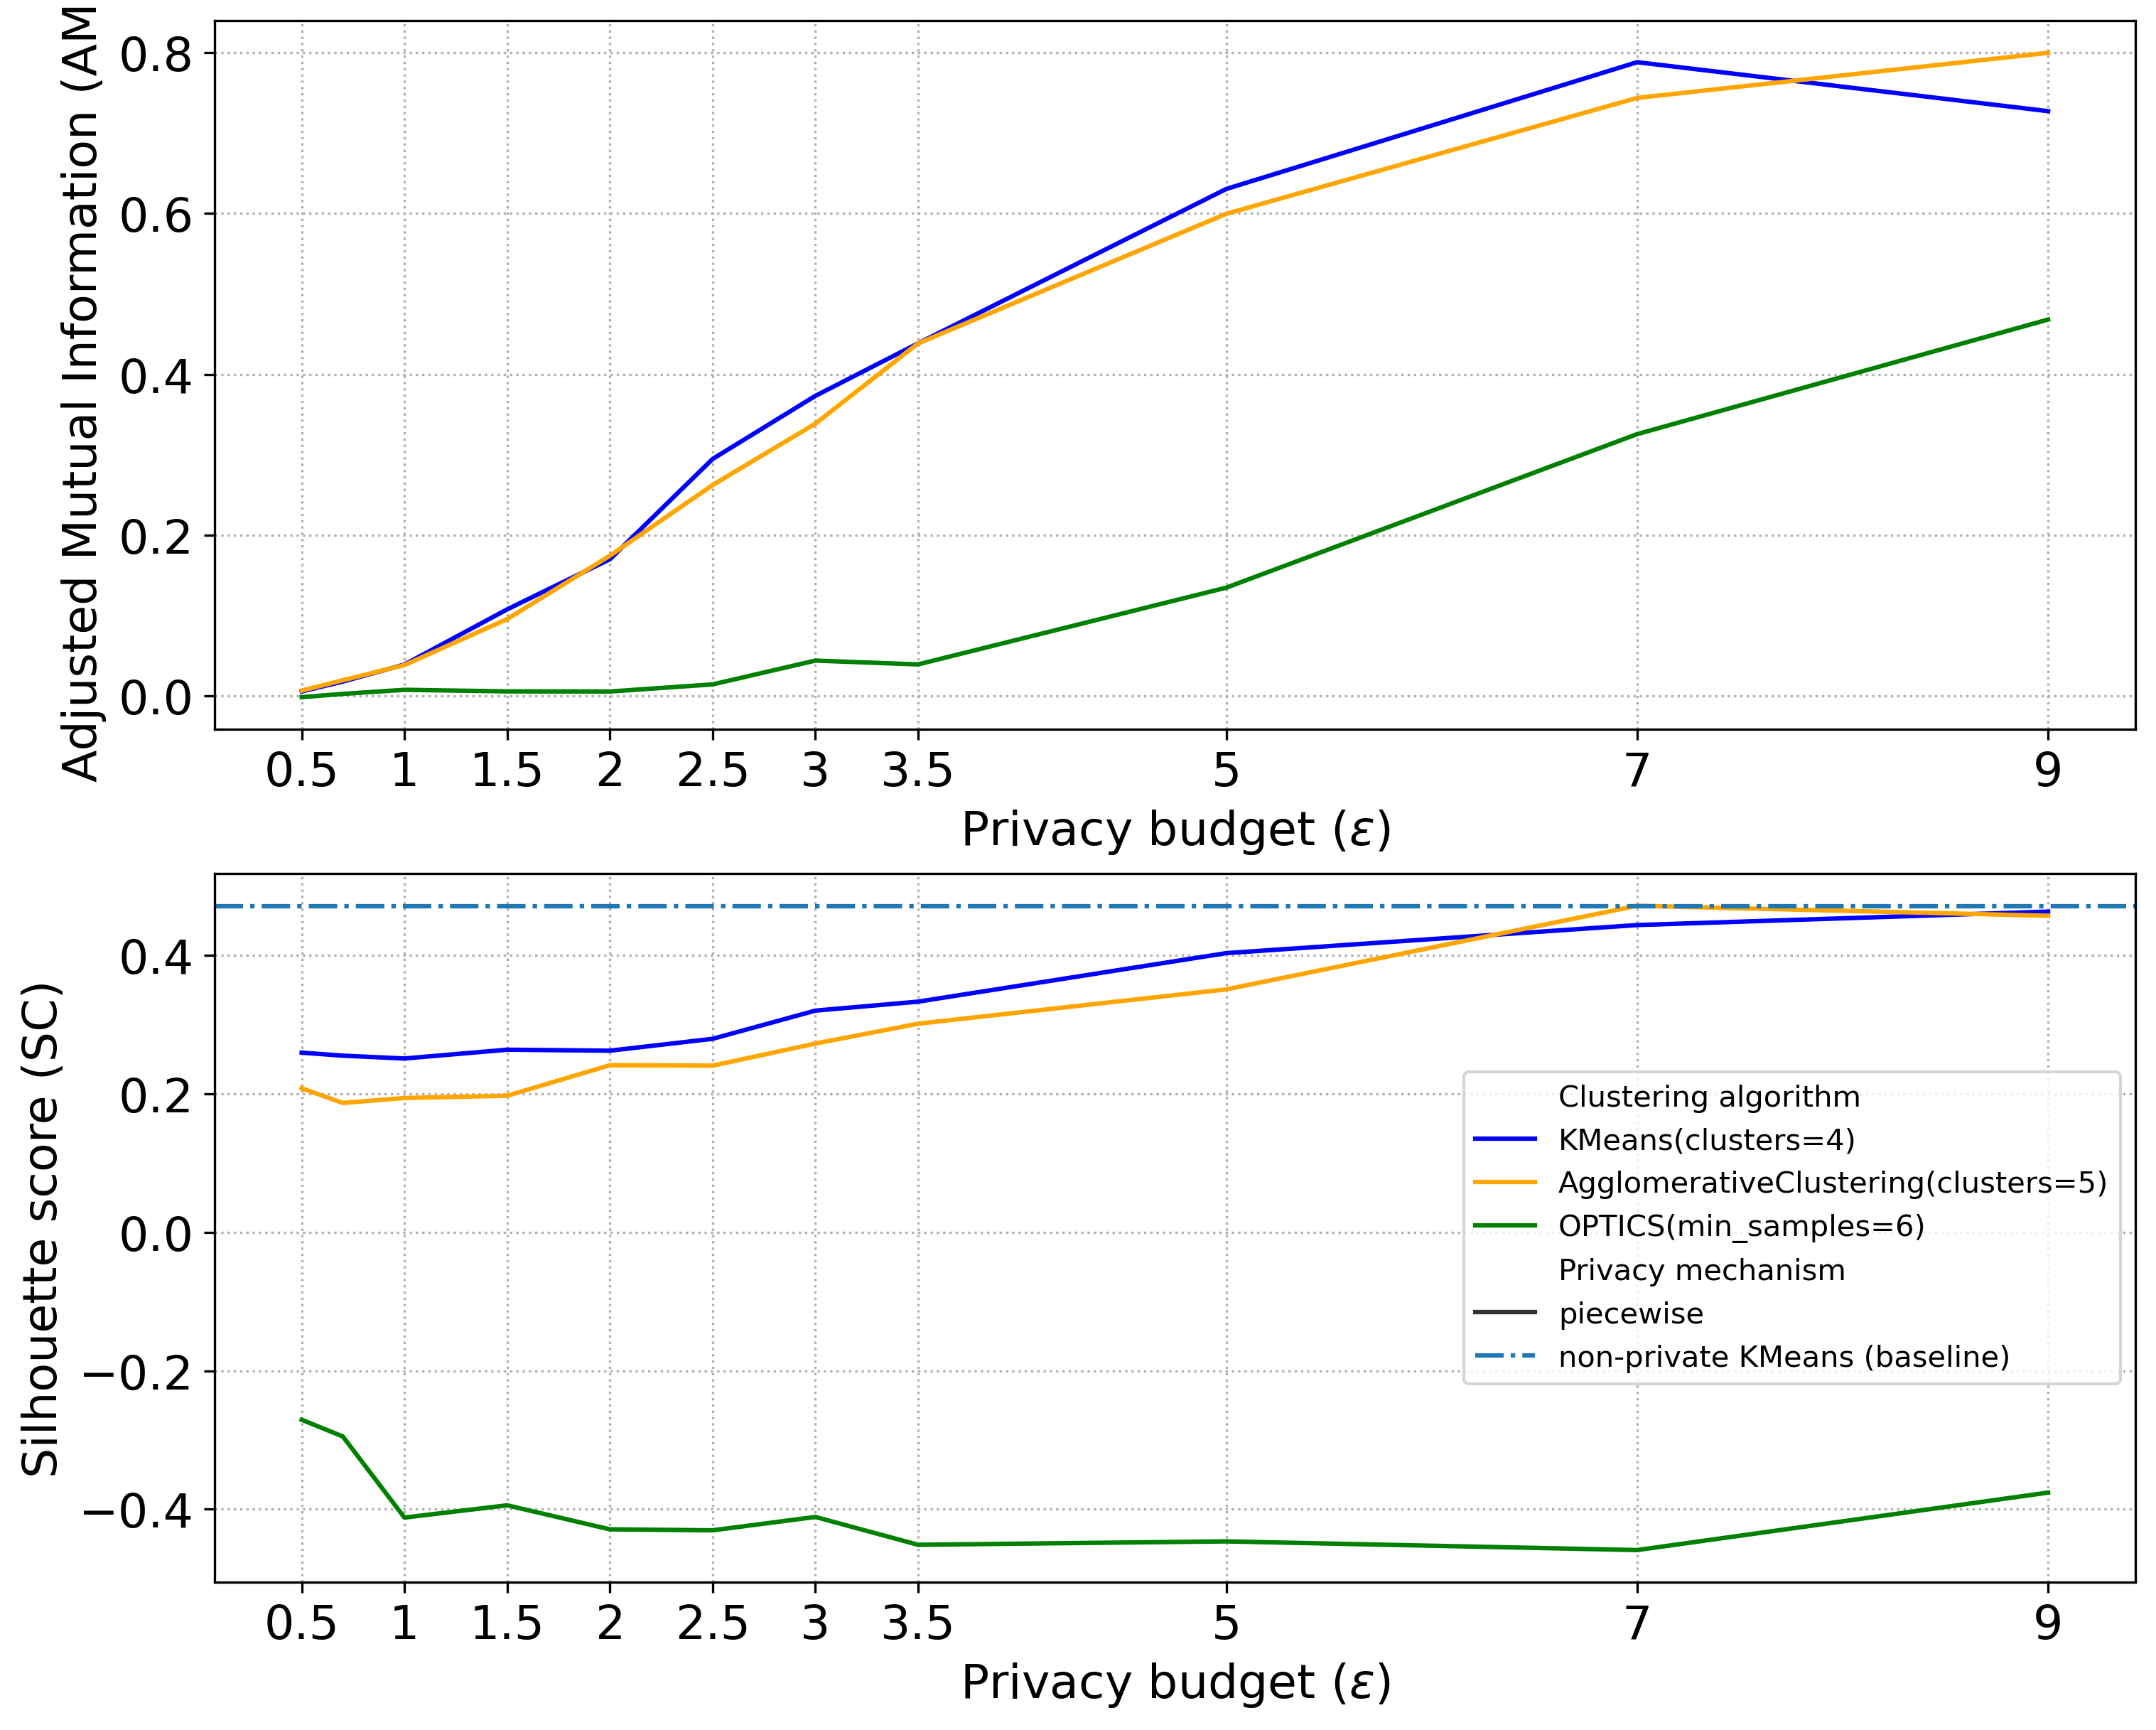
\includegraphics[width=0.65\textwidth]{Results/kd-laplace/piecewise/line-dataset/ami-and-sc_3_dimensions.png}
      \end{subfigure}
      \label{fig:validation-line-dataset_comparison_3d-laplace}
\end{figure}
K-Means performs best with kD-Laplace, scoring 0.6 \gls{ami} from privacy budget 3.5 to 9.
\gls{ag} follows the same pattern but with around 0.2 \gls{ami} lower.
\gls{optics} scores poorly (< 0.1 \gls{ami}).
Piecewise shows a similar trend as kD-Laplace, with slightly higher scores. \gls{optics} improves to 0.43 \gls{ami} at privacy budget 9.
Both mechanisms are similar for \gls{sc}, with Piecewise slightly higher, while \gls{optics} remains relatively lower.
\newpage
\begin{figure}[H]
      \centering
      \begin{subfigure}{0.3\textwidth}
            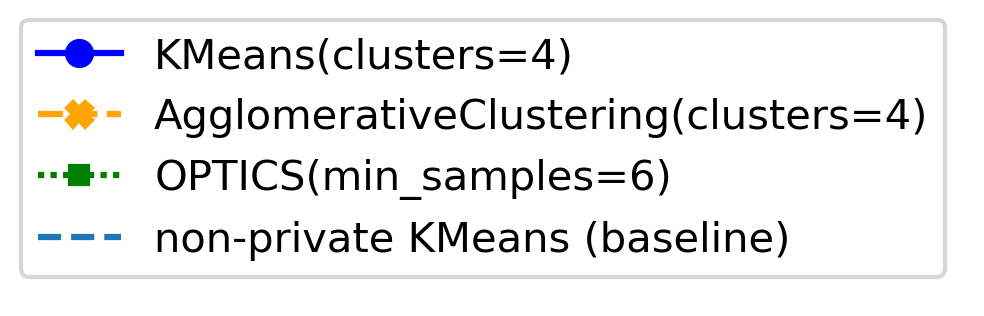
\includegraphics[width=\textwidth]{Results/kd-laplace/kd-Laplace/skewed-dataset/legend_3.png}
      \end{subfigure}
      \begin{subfigure}{1\textwidth}
            \caption{\textbf{AMI (top) and SC (bottom) for the kD-Laplace mechanism for the 3-dimensional data skewed-dataset}}
            \centering
            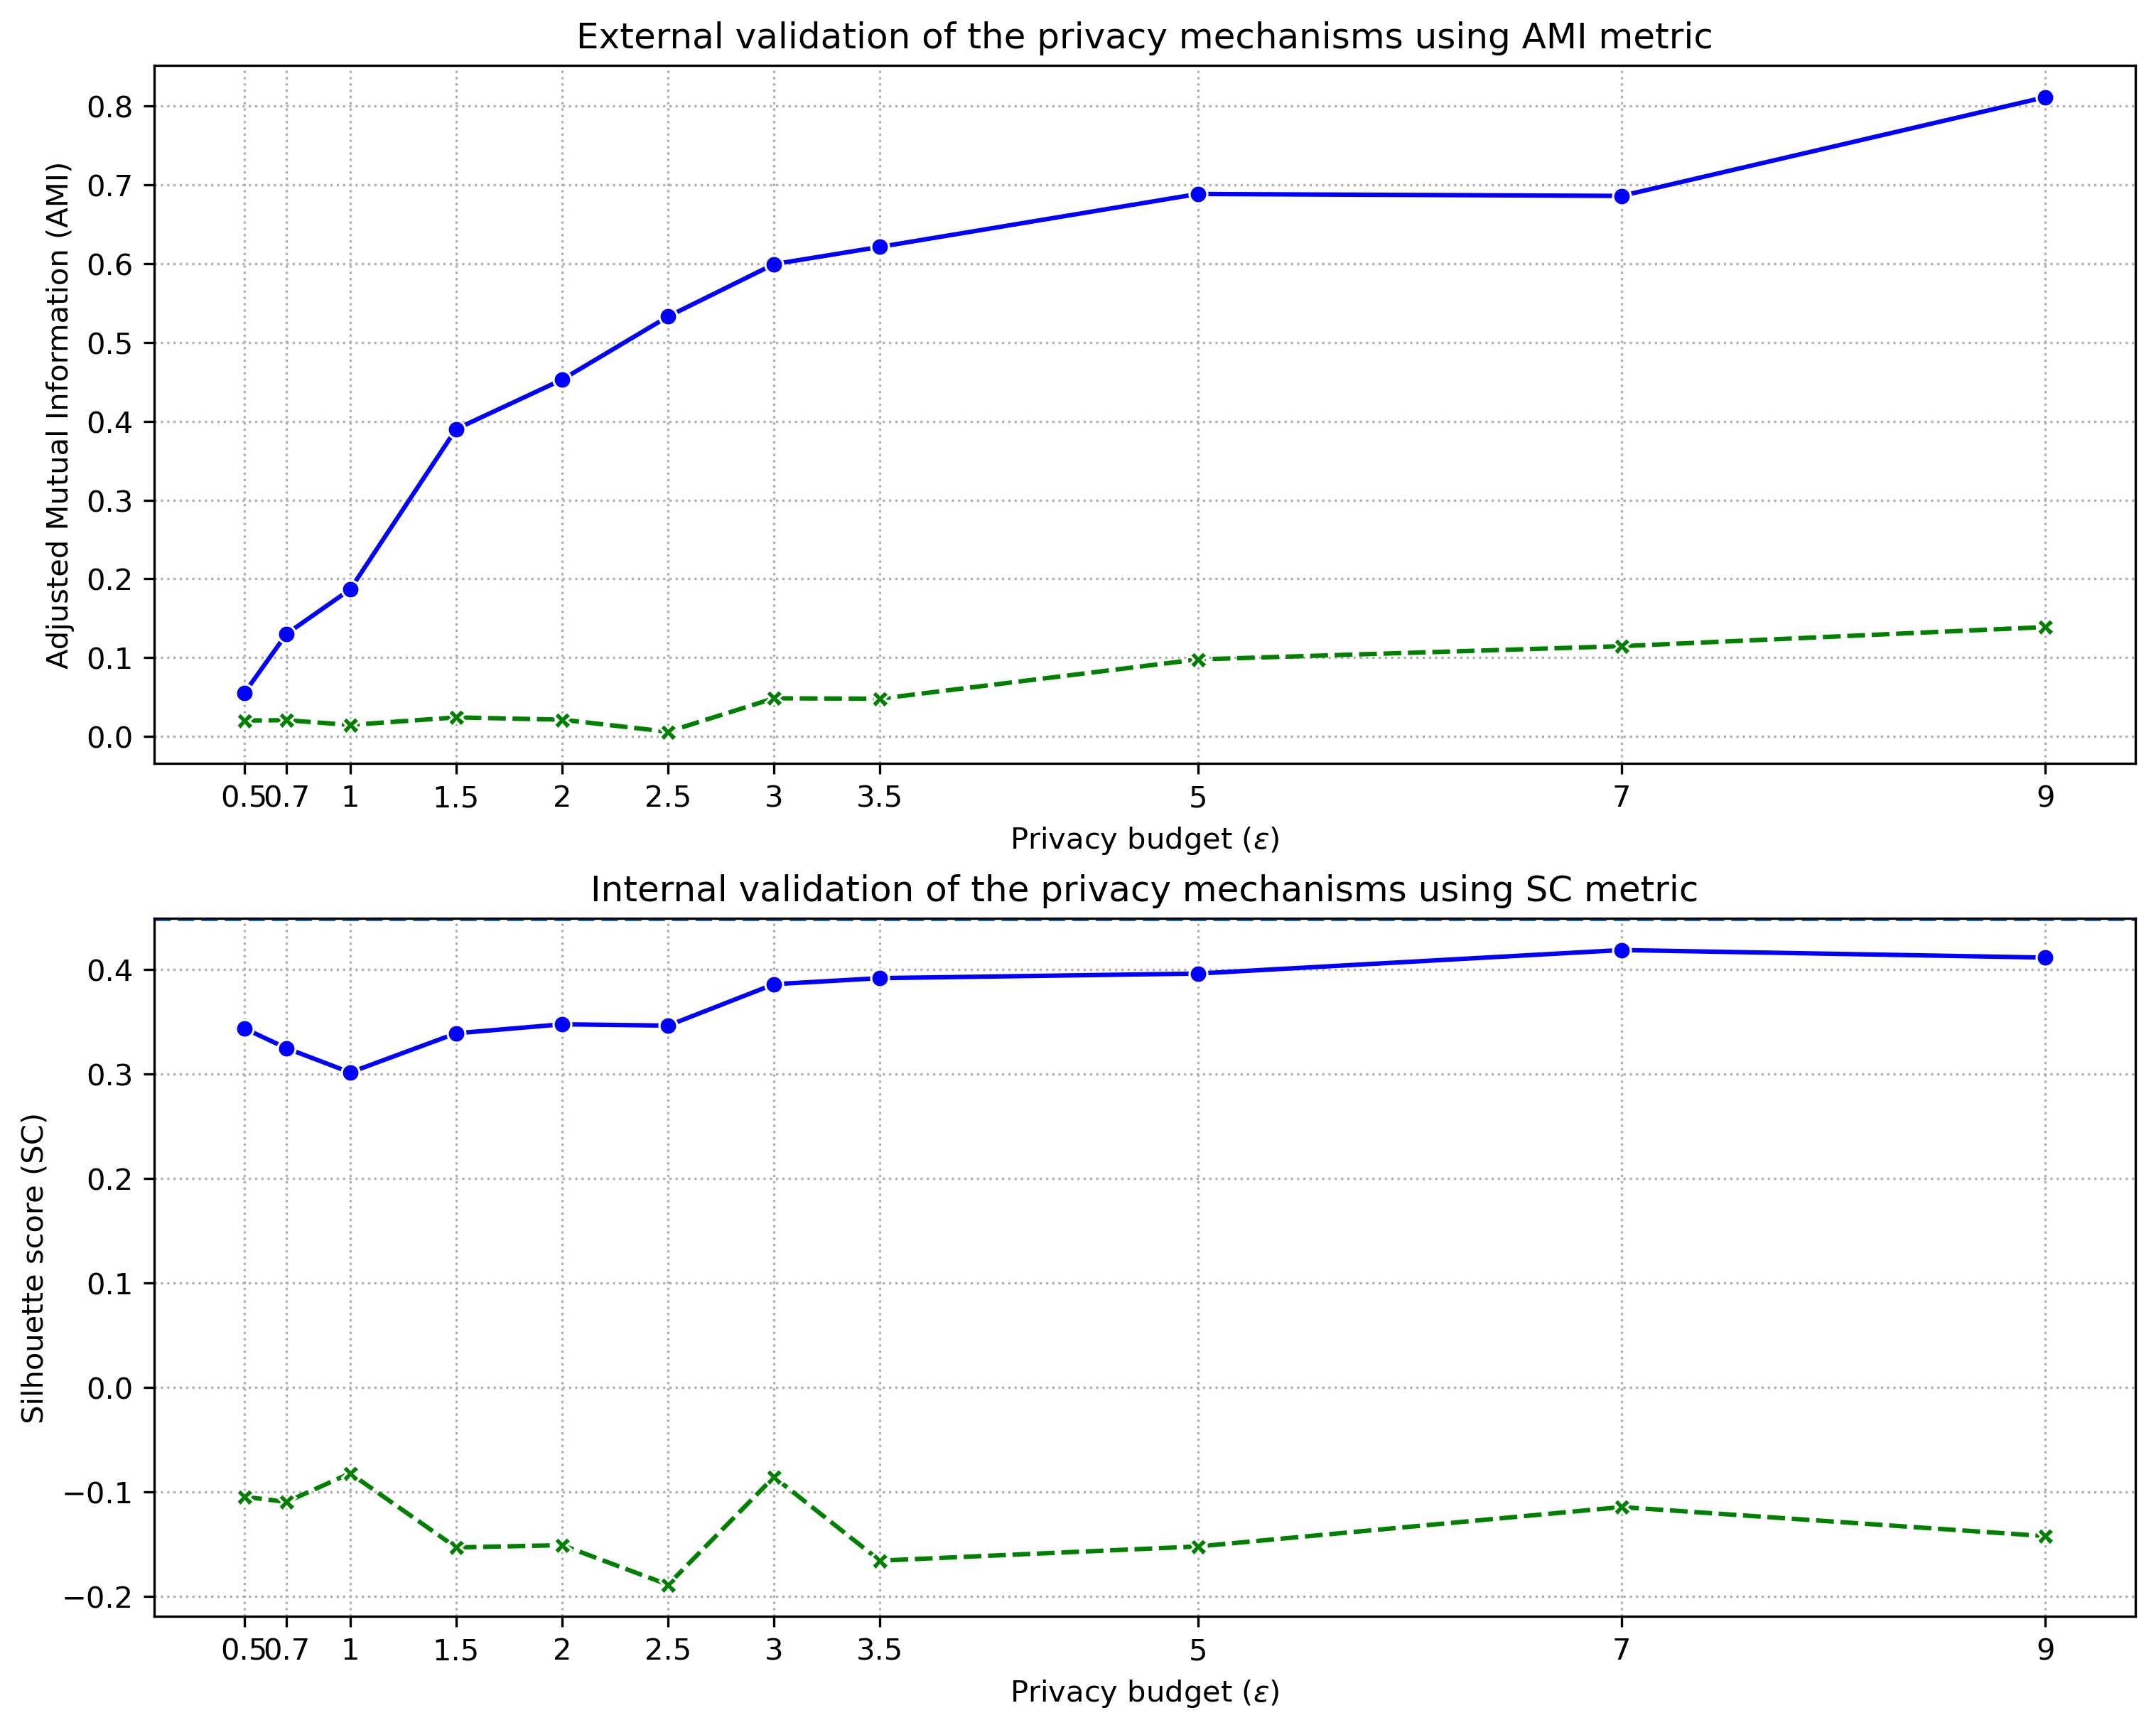
\includegraphics[width=0.65\textwidth]{Results/kd-laplace/kd-Laplace/skewed-dataset/ami-and-sc_3_dimensions.png}
            \centering
      \end{subfigure}
      \begin{subfigure}{1\textwidth}
            \caption{\textbf{AMI (top) and SC (bottom) for the Piecewise mechanism for the 3-dimensional data skewed-dataset}}
            \centering
            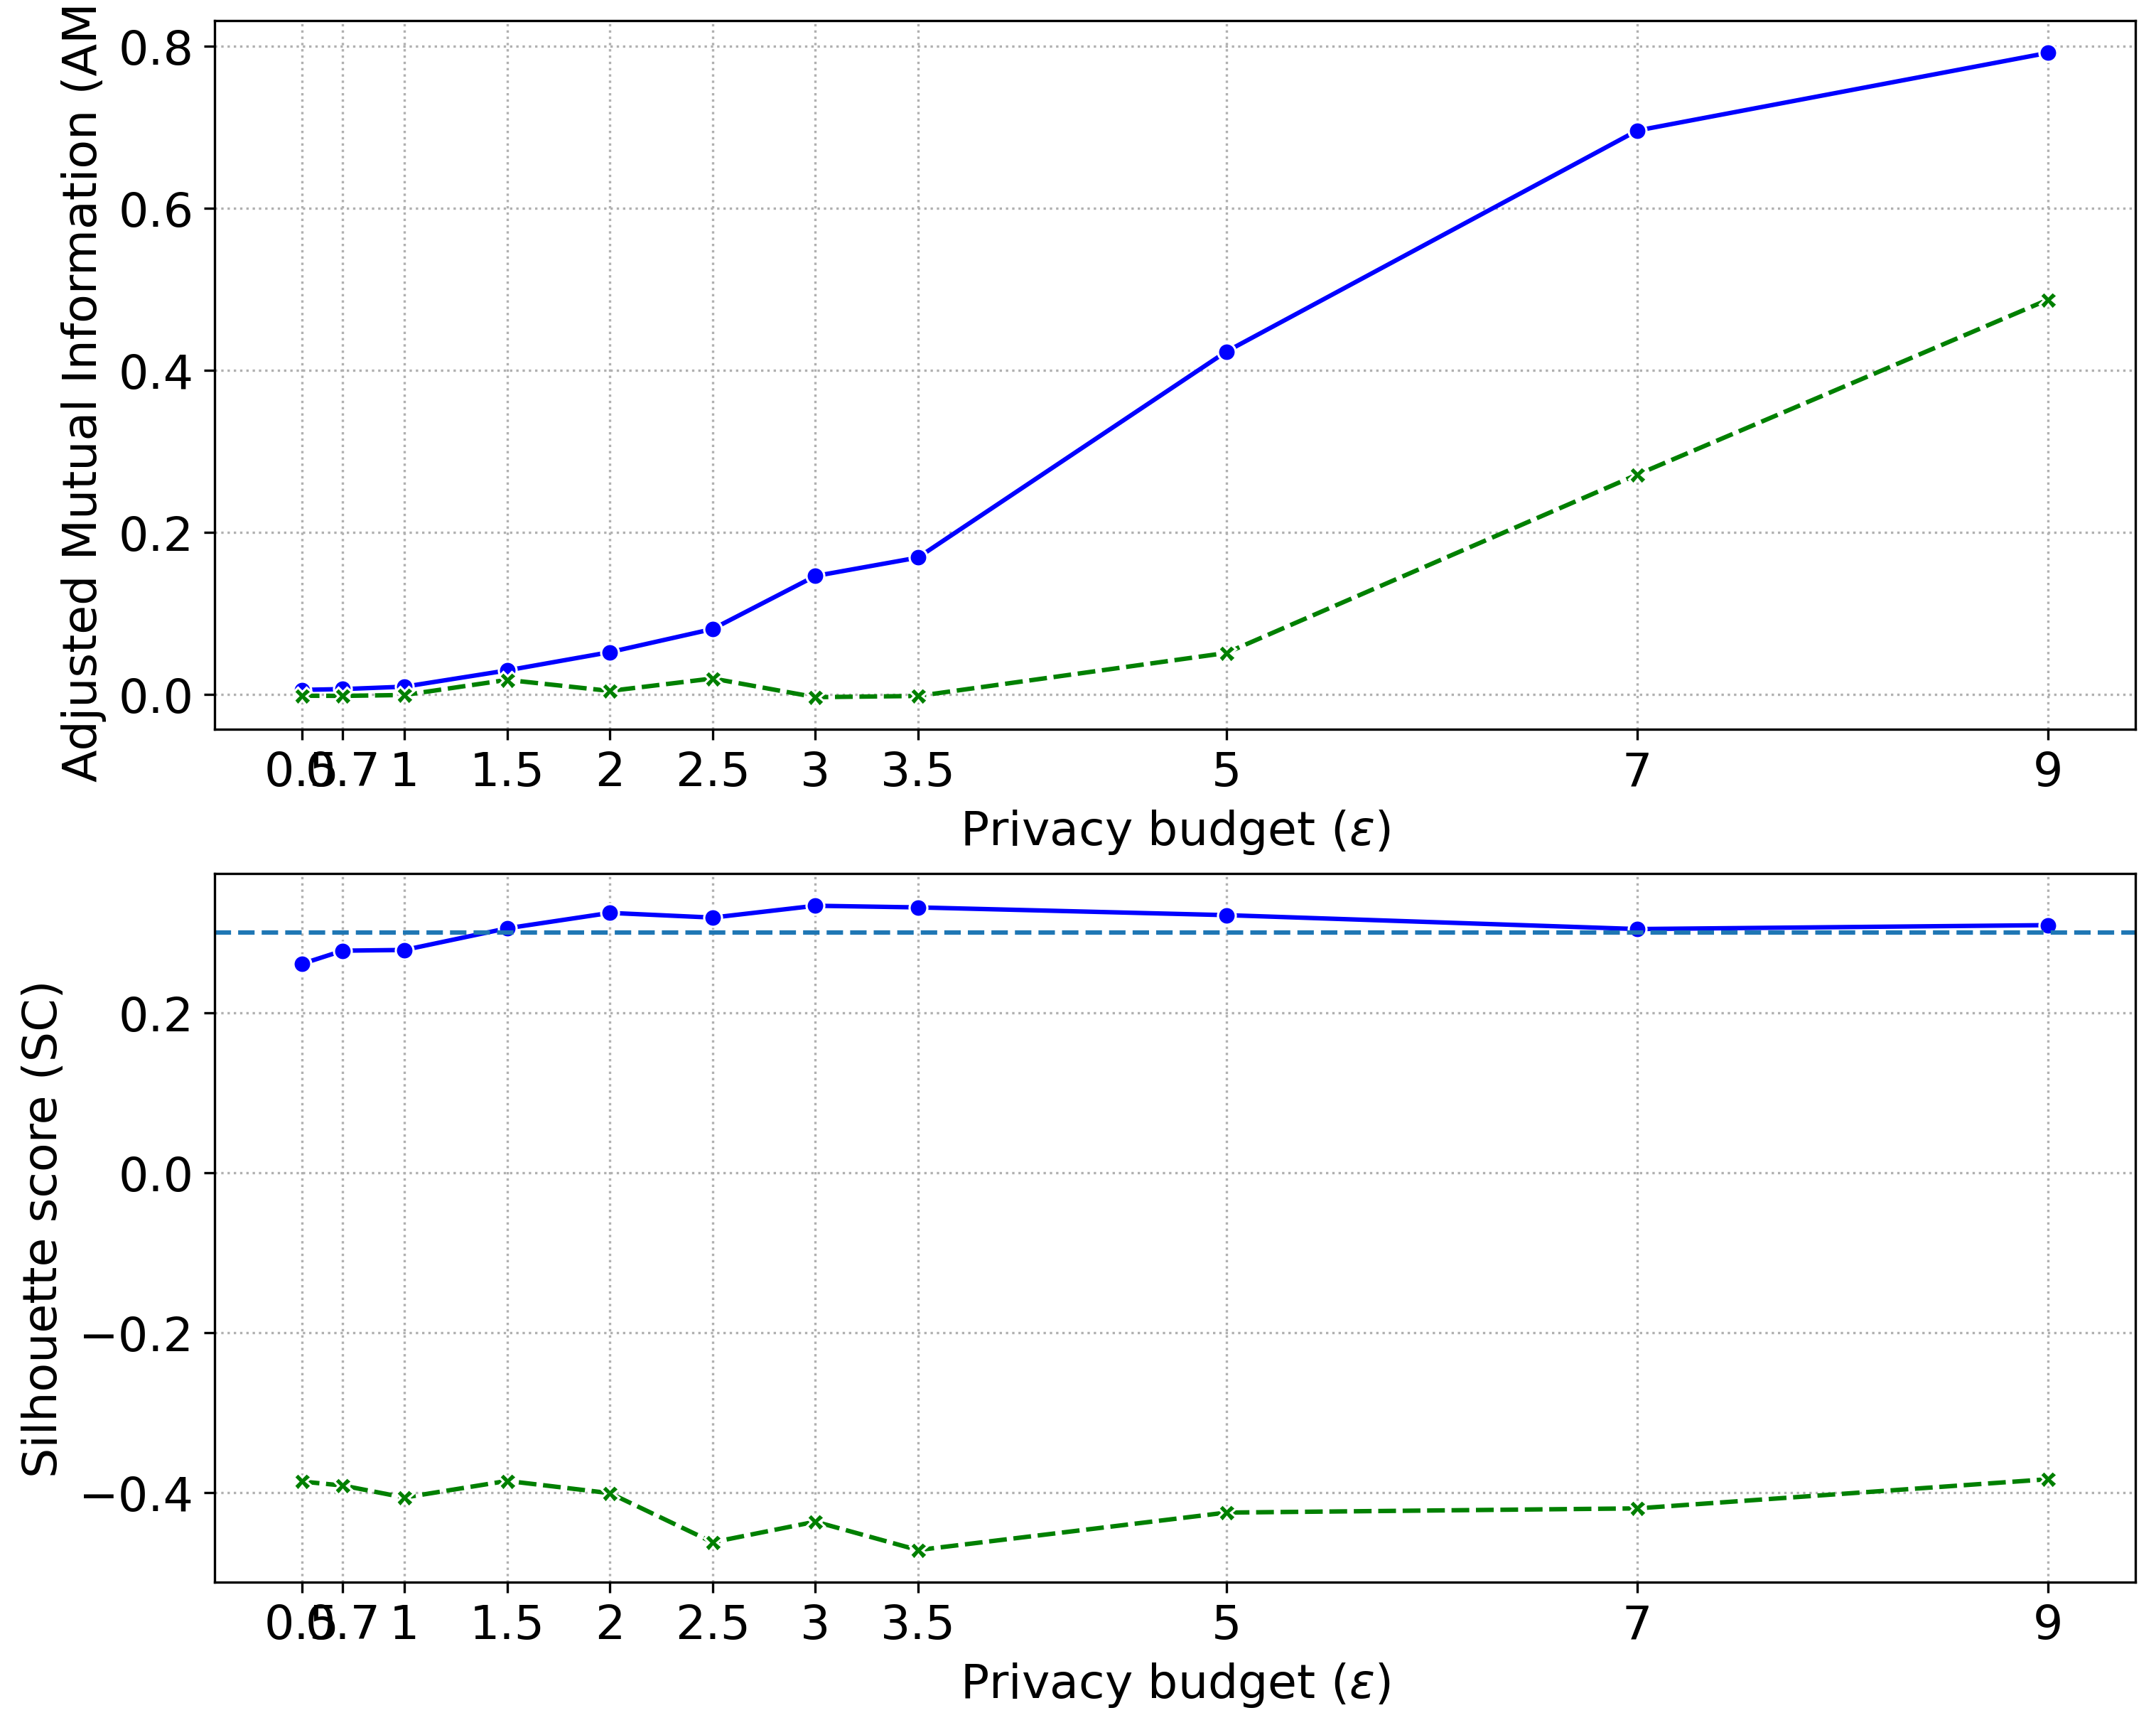
\includegraphics[width=0.65\textwidth]{Results/kd-laplace/piecewise/skewed-dataset/ami-and-sc_3_dimensions.png}
      \end{subfigure}
      \label{fig:validation-skewed-dataset_comparison_3d-laplace}
\end{figure}
kD-Laplace scores best with the K-Means algorithm, 0.59 \gls{ami} for privacy budget 9.
In contrast, \gls{ag} is +/- 0.3 for privacy budgets 7 and 9. \gls{optics} scores worst with a maximum value of 0.02 \gls{ami}.
The Piecewise mechanism scores much better with a \gls{ami} of 0.8 for K-Means. The same trend is observed for \gls{ag} and \gls{optics} as with kD-Laplace.
Both score worse, but \gls{optics} scores equal to \gls{ag} for privacy budget 9.
Both mechanisms score equal for the \gls{sc}, but Piecewise is slightly higher and scores equal to the baseline.
\newpage
\subsection{n-dimensional data}
\begin{figure}[H]
      \centering
      \begin{subfigure}{0.30\textwidth}
            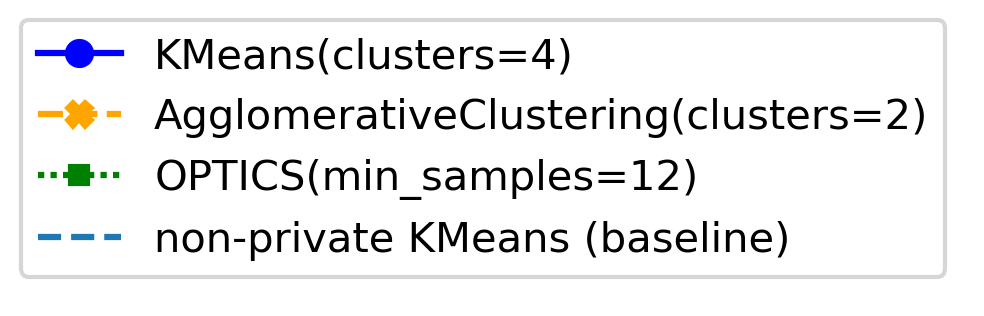
\includegraphics[width=\textwidth]{Results/kd-laplace/kd-Laplace/seeds-dataset/legend_7.png}
      \end{subfigure}
      \begin{subfigure}{1\textwidth}
            \caption{\textbf{AMI (top) and SC (bottom) for the kD-Laplace mechanism for the n-dimensional data seeds-dataset}}
            \centering
            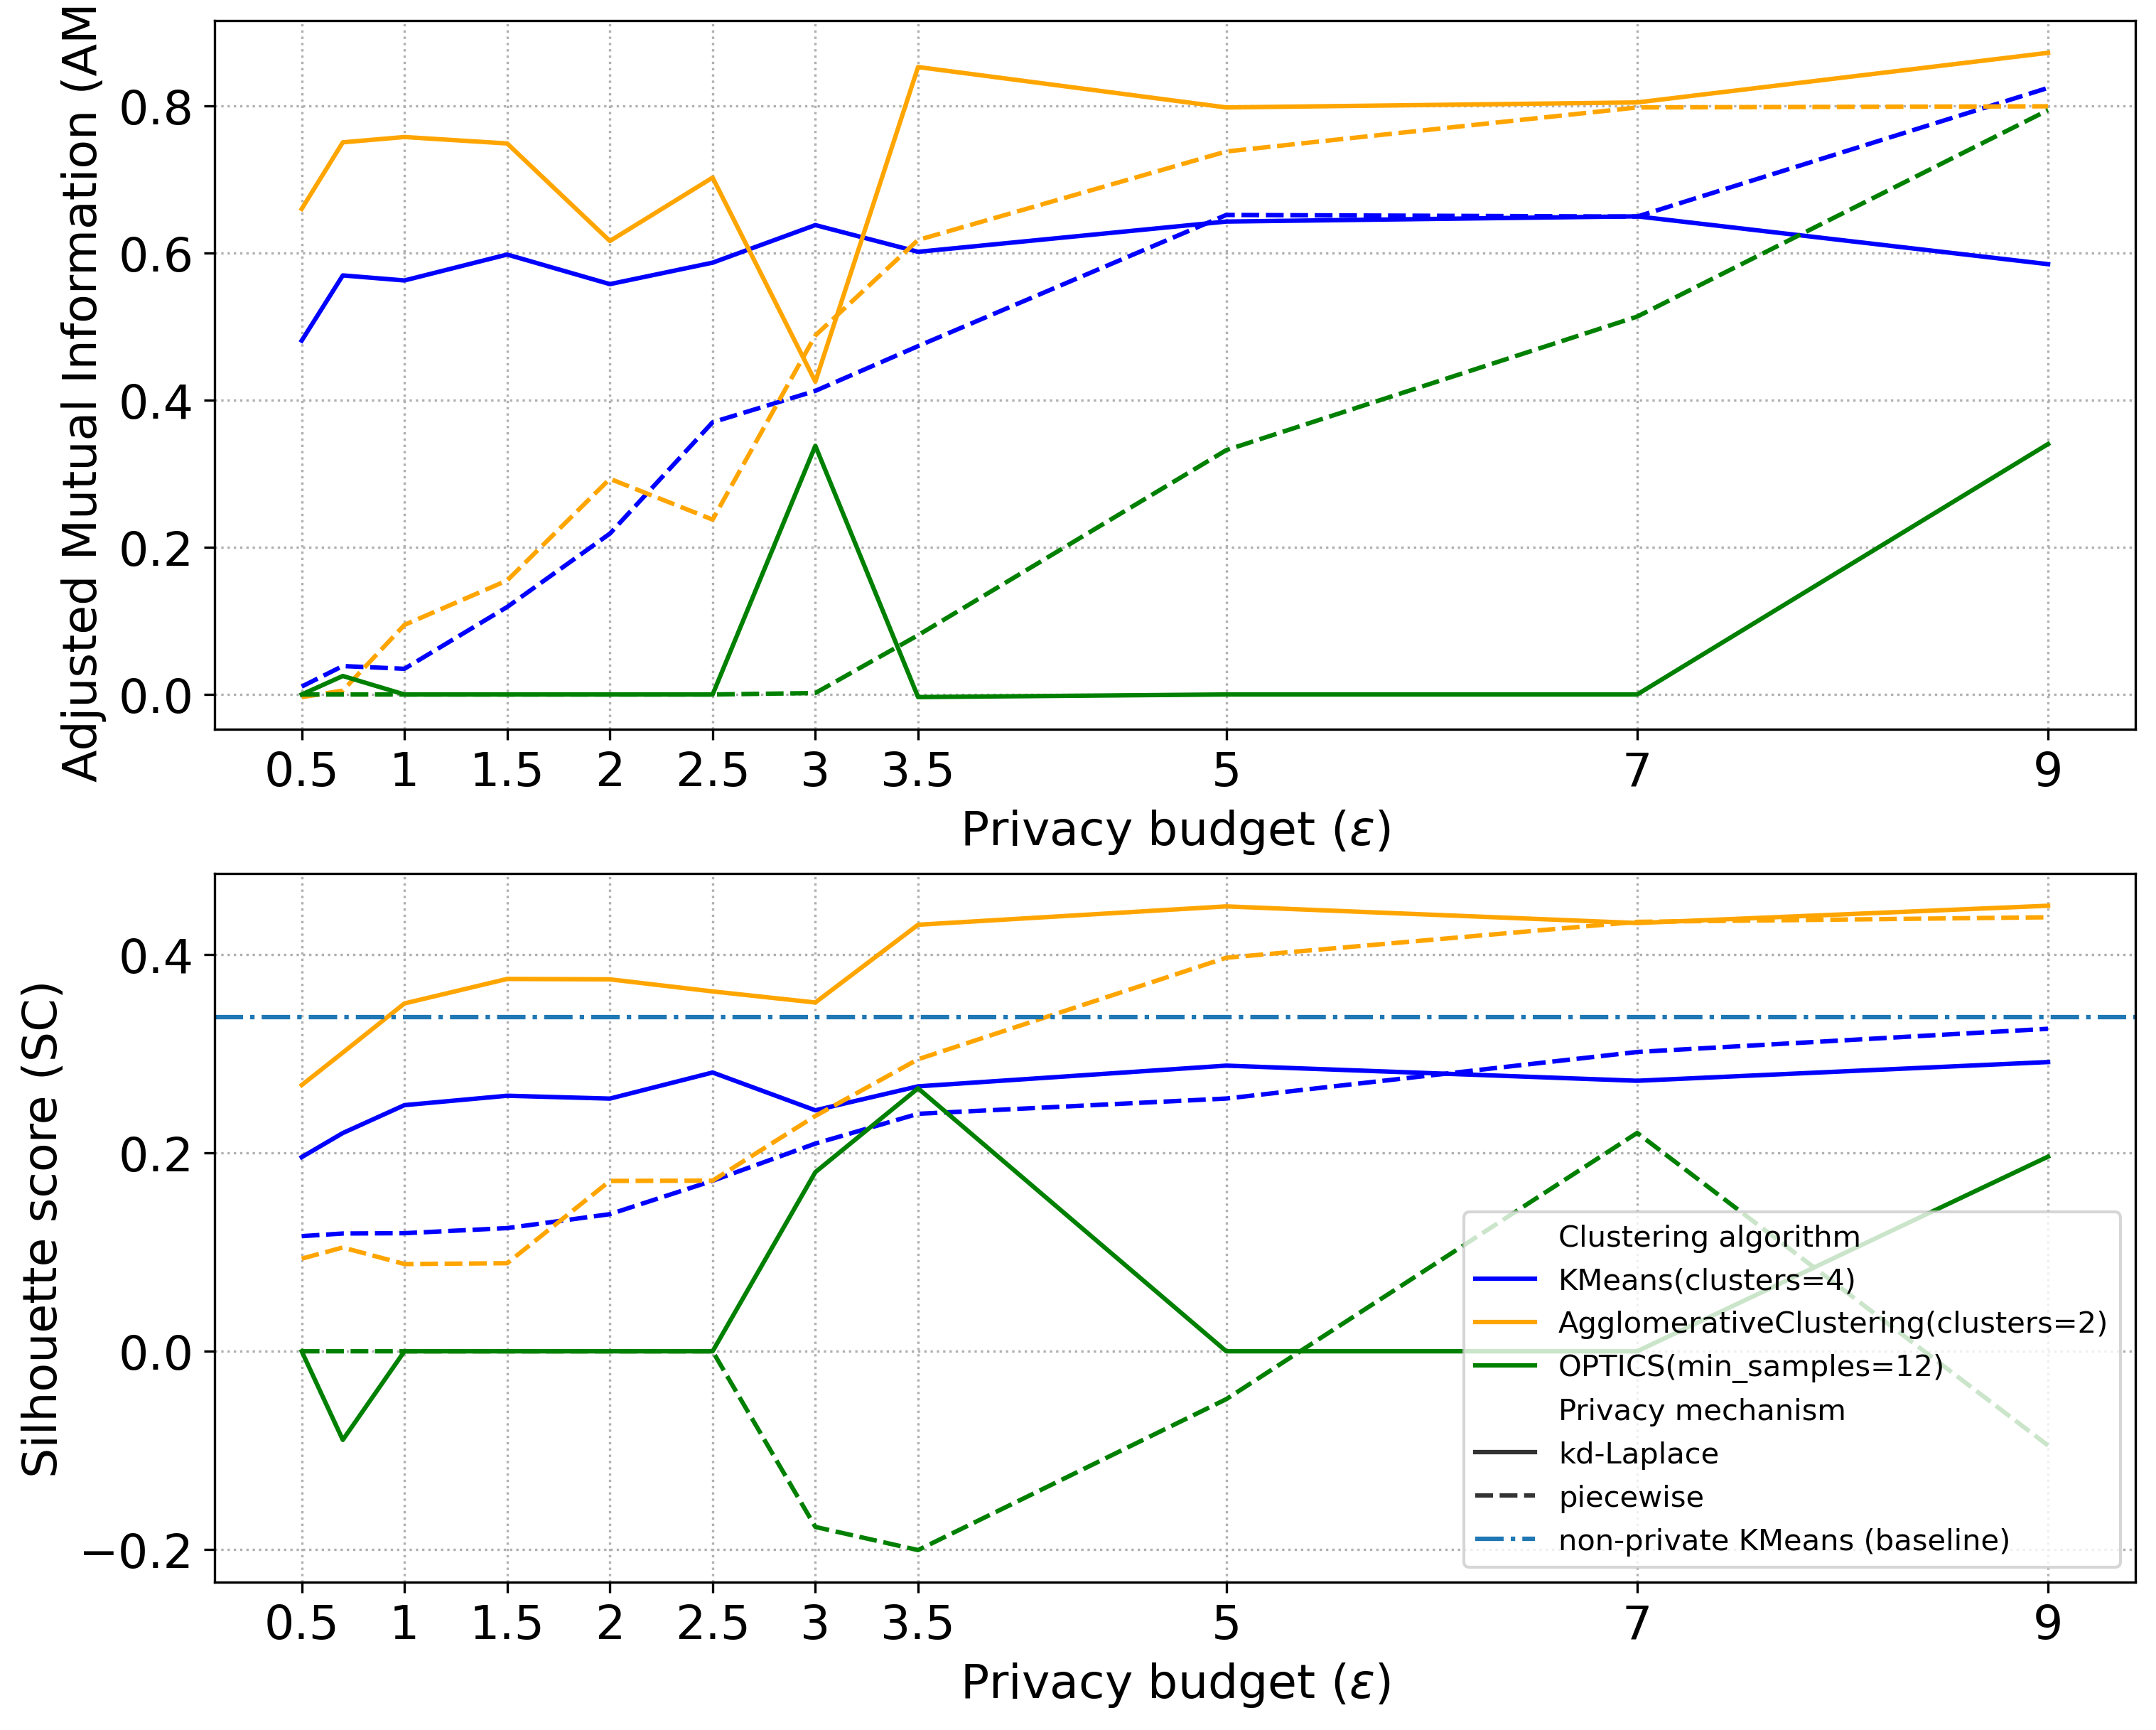
\includegraphics[width=0.65\textwidth]{Results/kd-laplace/kd-Laplace/seeds-dataset/ami-and-sc_7_dimensions.png}
            \centering
      \end{subfigure}
      \begin{subfigure}{1\textwidth}
            \caption{\textbf{AMI (top) and SC (bottom) for the Piecewise mechanism for the n-dimensional data seeds-dataset}}
            \centering
            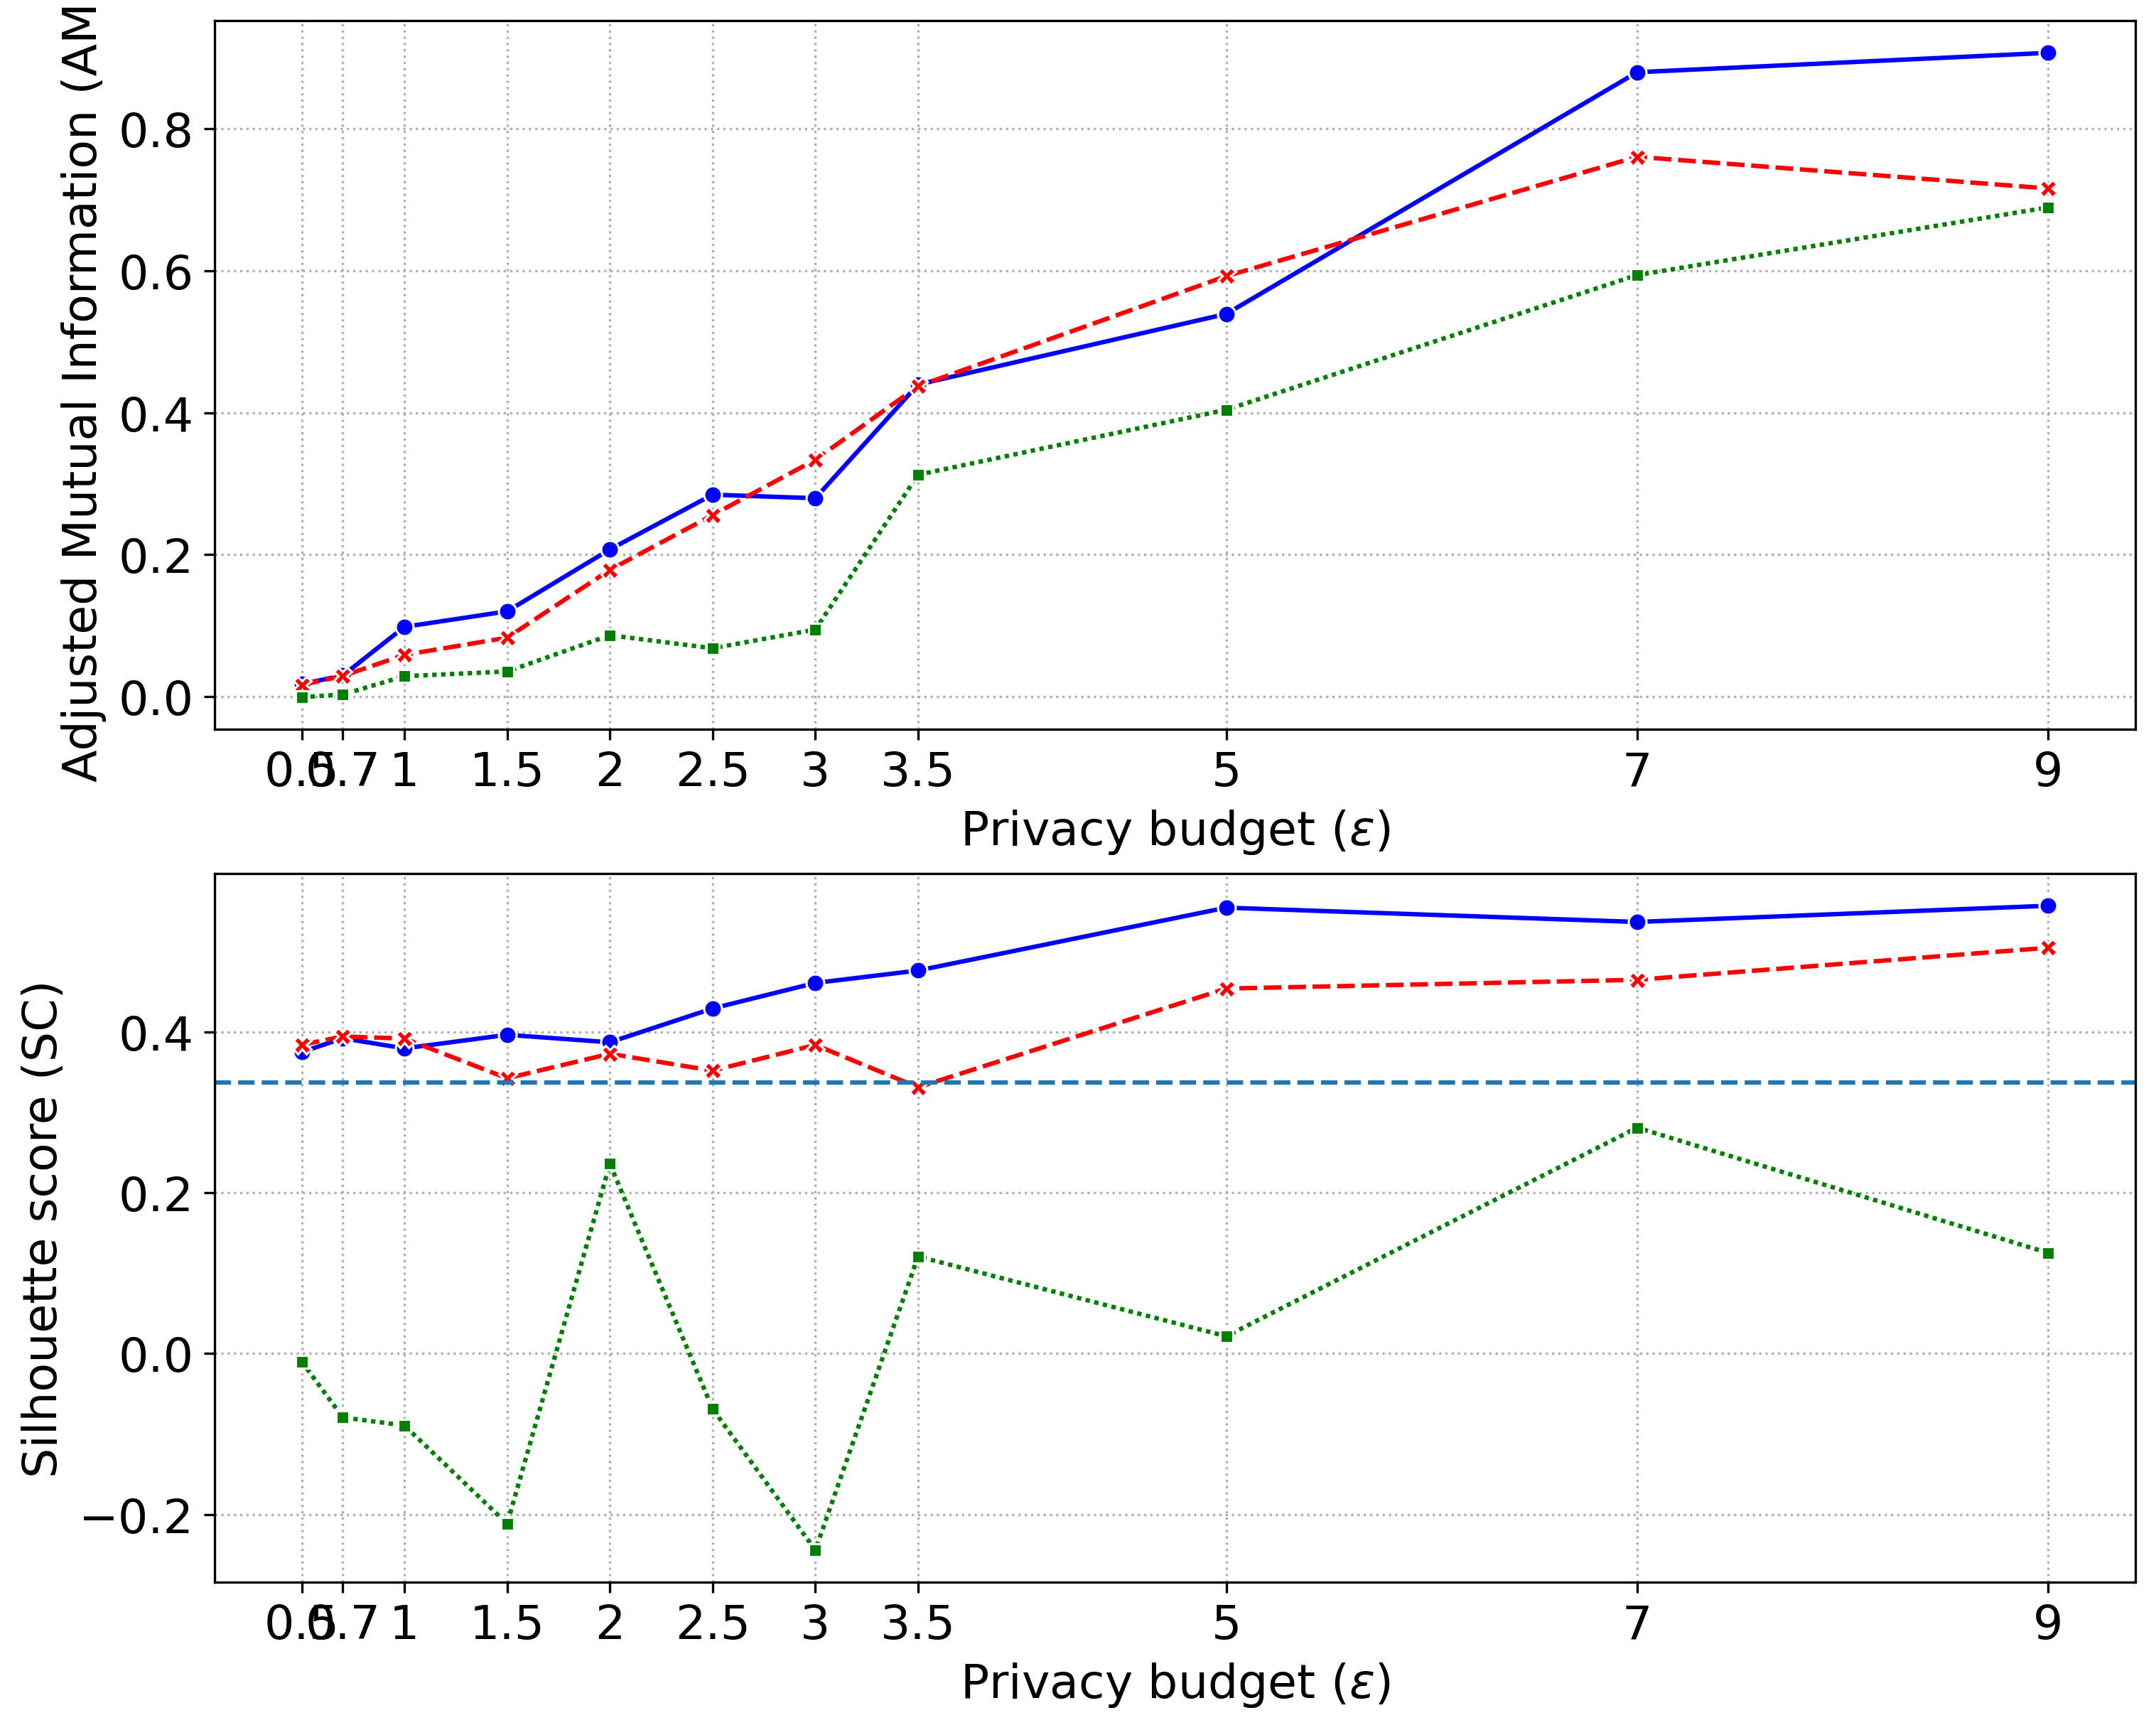
\includegraphics[width=0.65\textwidth]{Results/kd-laplace/piecewise/seeds-dataset/ami-and-sc_7_dimensions.png}
      \end{subfigure}
      \label{fig:validation-seeds-dataset_comparison_nd-laplace}
\end{figure}
kD-Laplace scores 0.83 \gls{ami} for \gls{ag} at privacy budget 9, while K-Means scores 0.5 to 0.6 \gls{ami} for all budgets.
Piecewise shows a similar trend, with all algorithms scoring nearly equal at budget 9. \gls{sc} follows a similar trend as \gls{ami}, with peaks at epsilon 3 and 3.5 for kD-Laplace with \gls{optics}. Overall, \gls{optics} scores lower for both mechanisms, with an upward trend for Piecewise but not for kD-Laplace.
\newpage
\begin{figure}[H]
      \centering
      \begin{subfigure}{0.30\textwidth}
            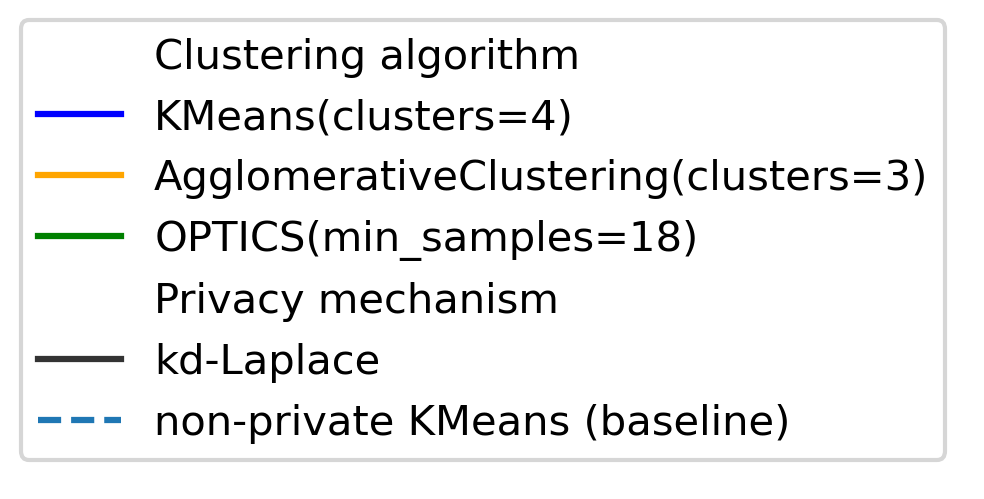
\includegraphics[width=\textwidth]{Results/kd-laplace/kd-Laplace/heart-dataset/legend_9.png}
      \end{subfigure}
      \begin{subfigure}{1\textwidth}
            \caption{\textbf{AMI (top) and SC (bottom) for the kD-Laplace mechanism for the n-dimensional data heart-dataset}}
            \centering
            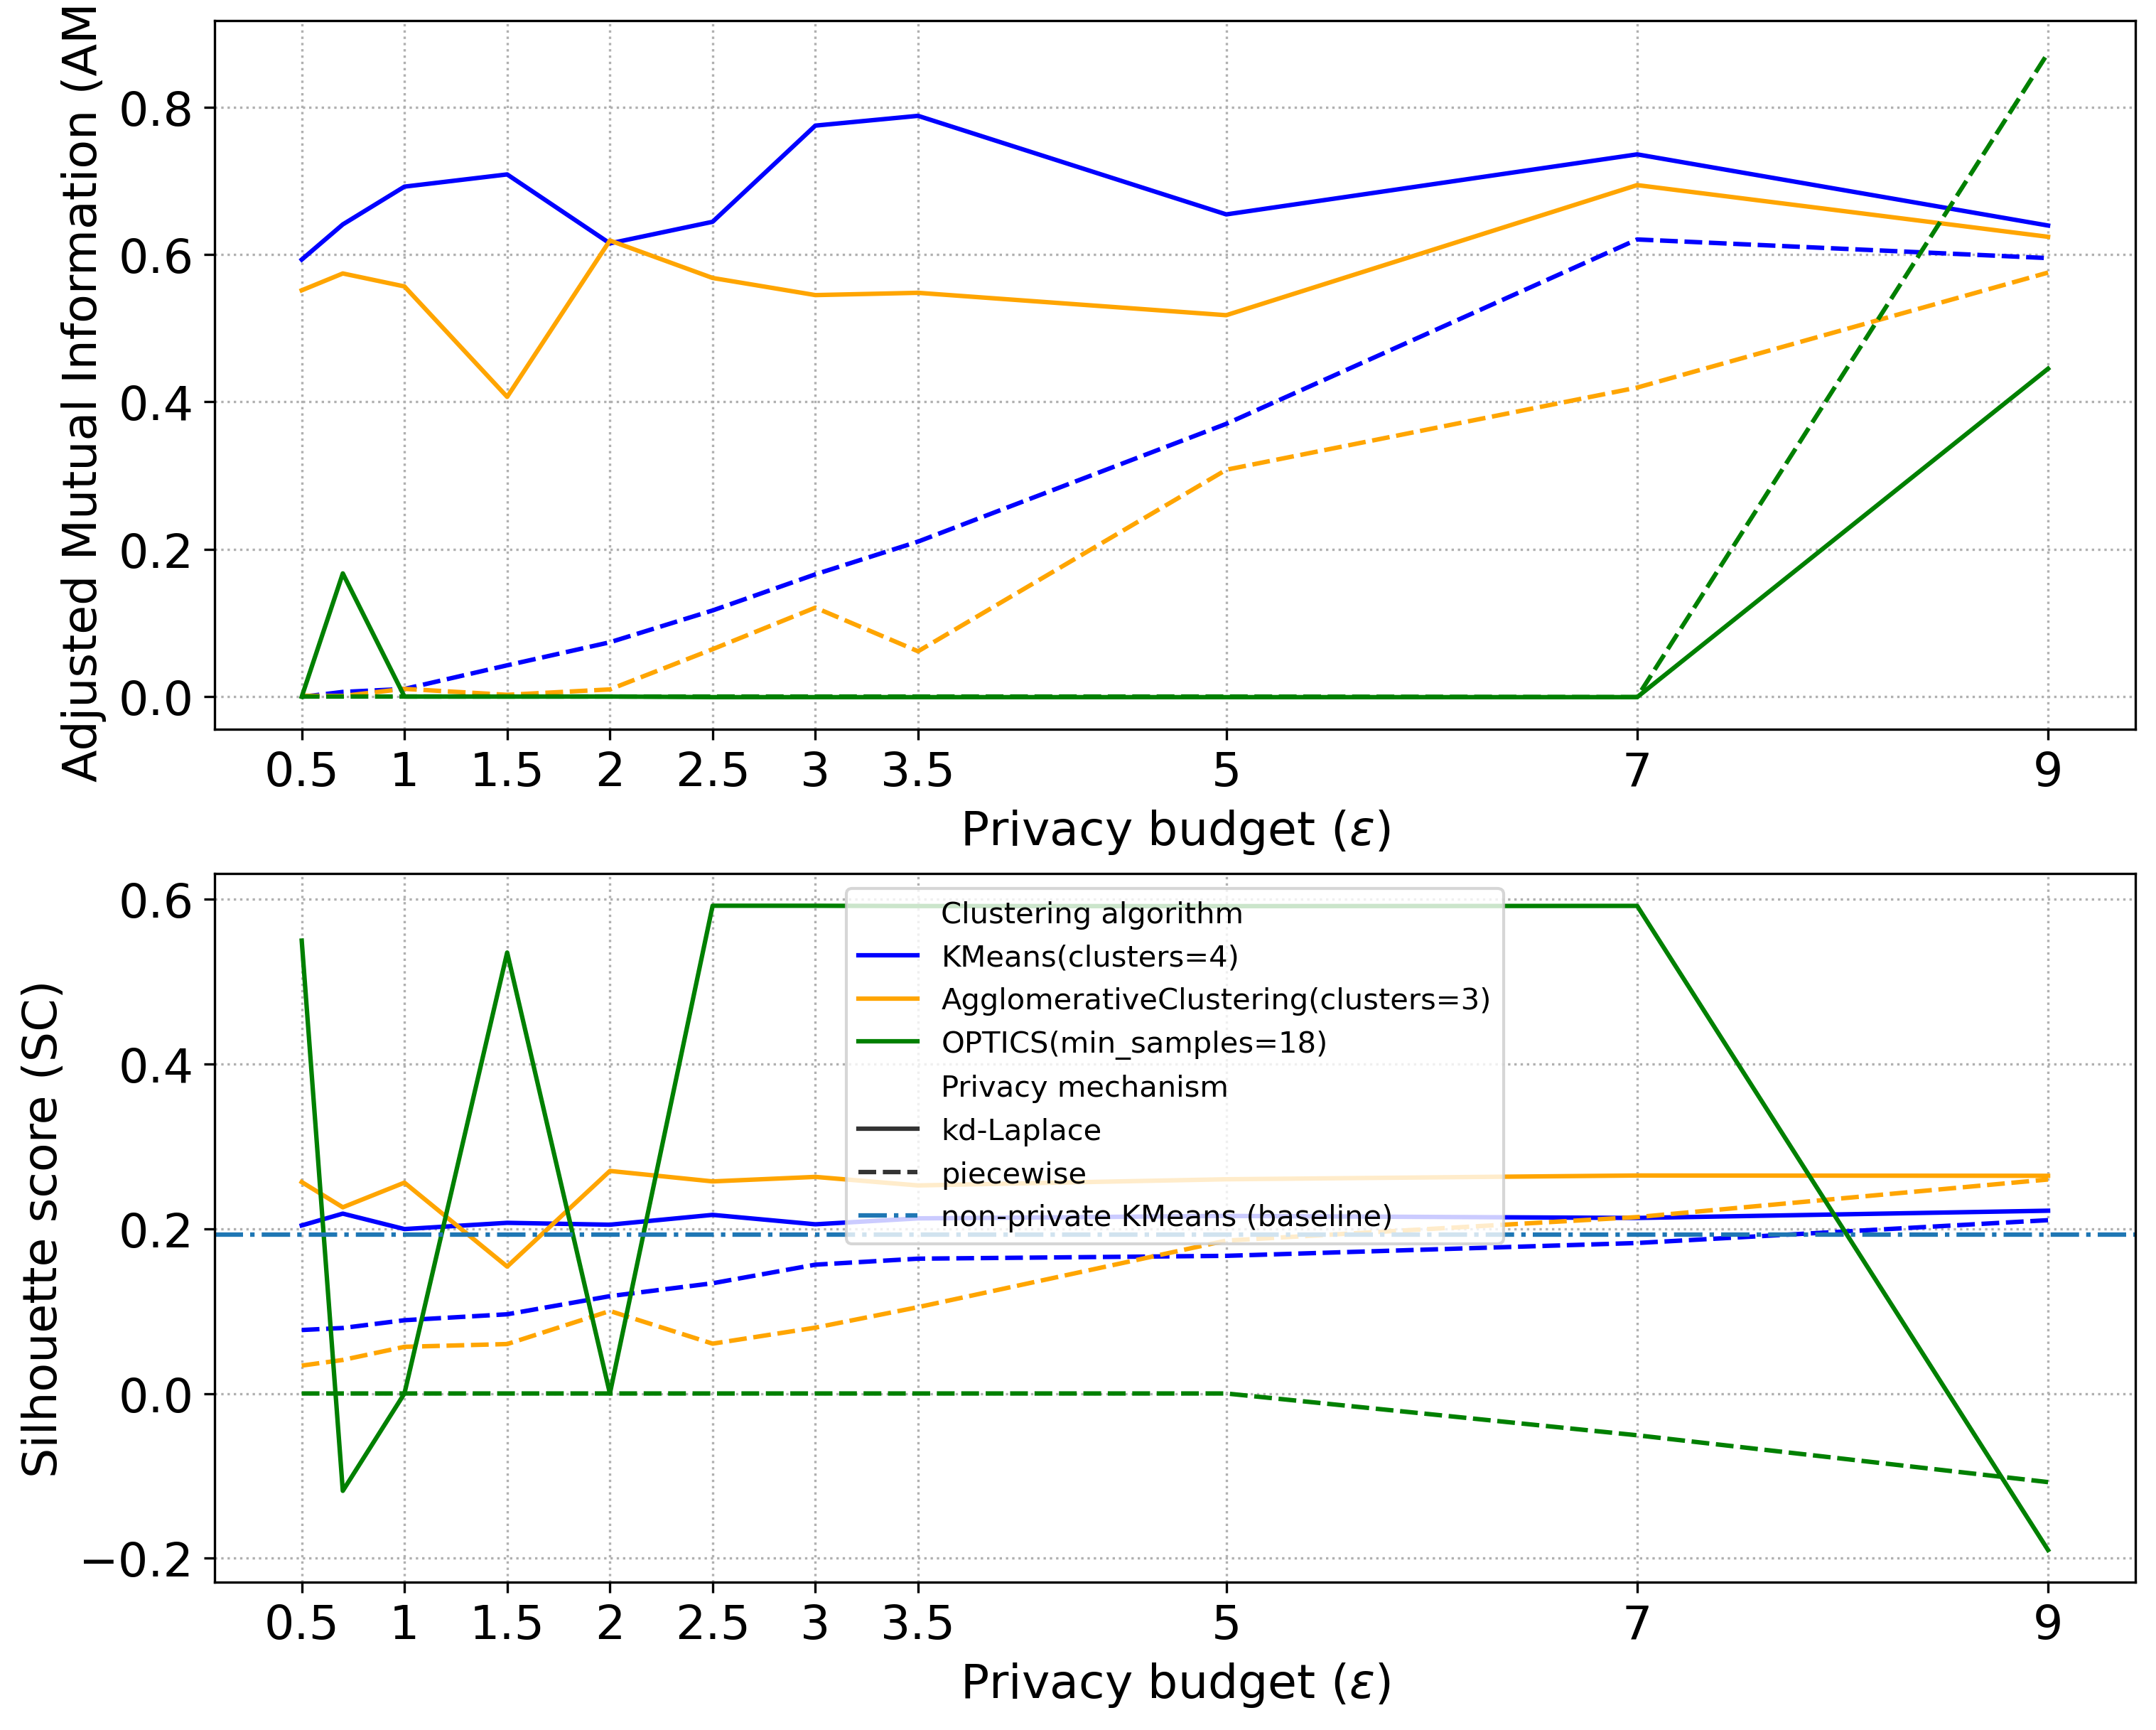
\includegraphics[width=0.65\textwidth]{Results/kd-laplace/kd-Laplace/heart-dataset/ami-and-sc_9_dimensions.png}
            \centering
      \end{subfigure}
      \begin{subfigure}{1\textwidth}
            \caption{\textbf{AMI (top) and SC (bottom) for the Piecewise mechanism for the n-dimensional data heart-dataset}}
            \centering
            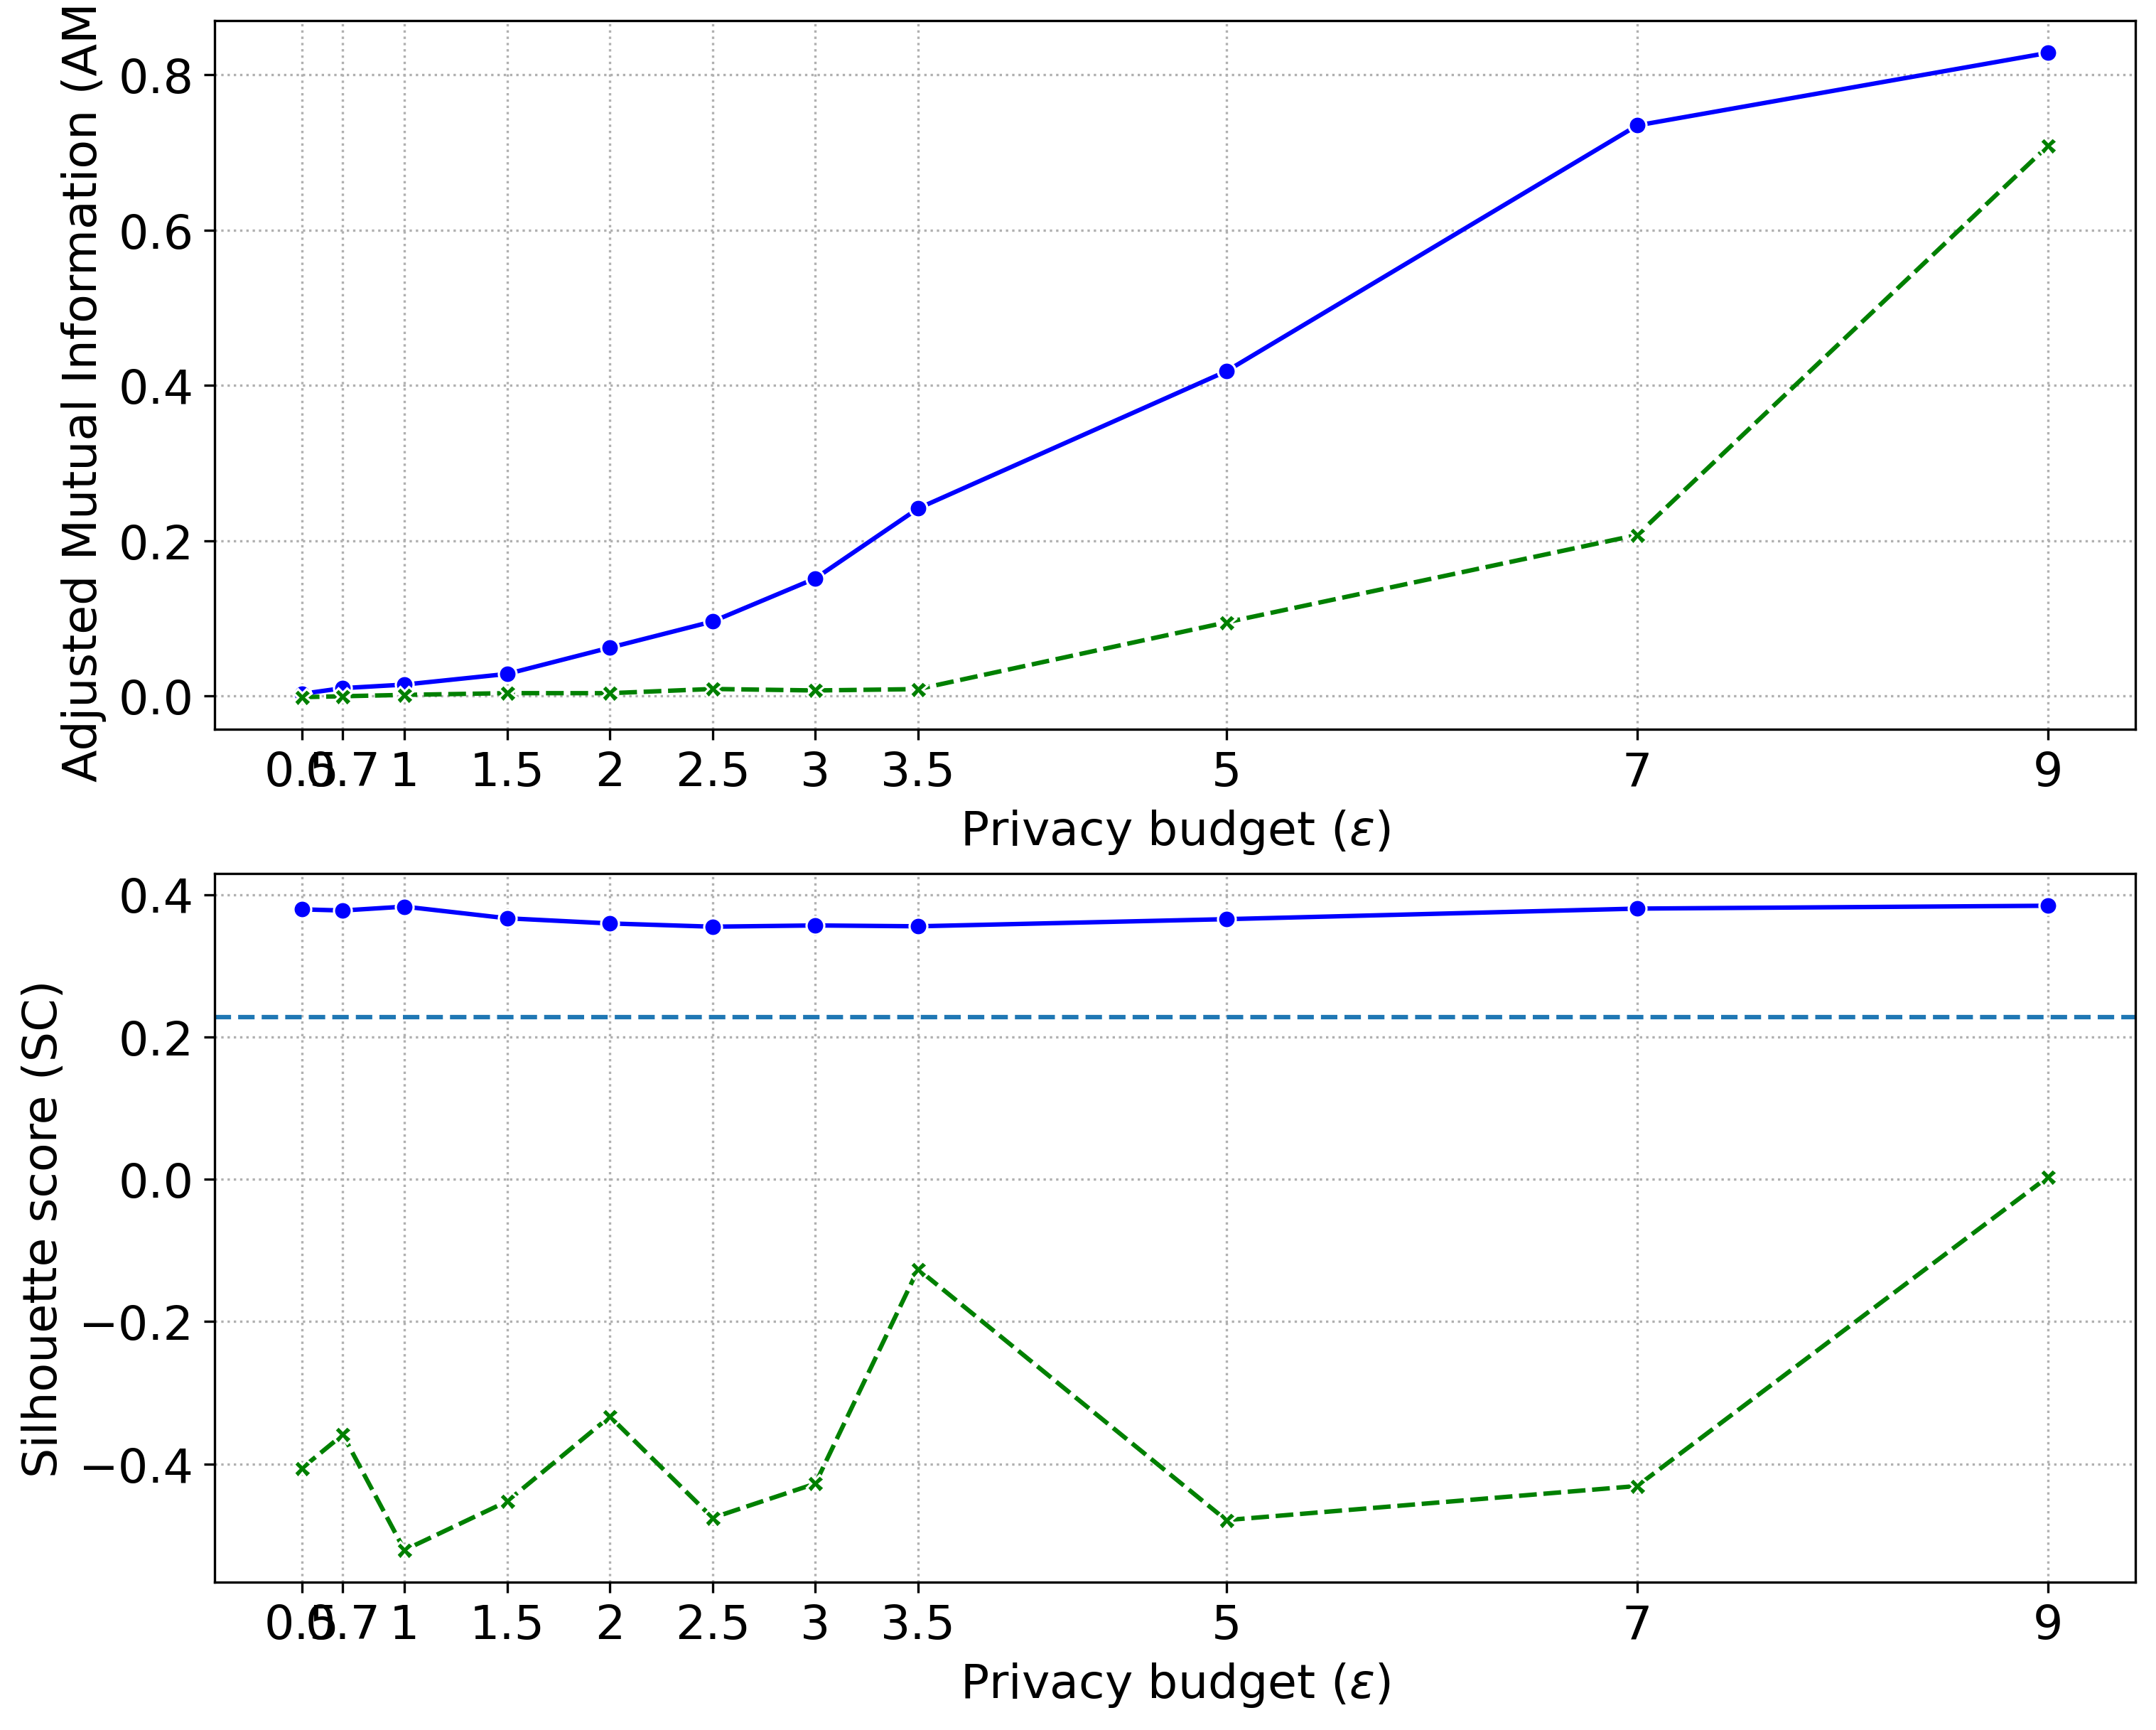
\includegraphics[width=0.65\textwidth]{Results/kd-laplace/piecewise/heart-dataset/ami-and-sc_9_dimensions.png}
      \end{subfigure}
      \label{fig:validation-heart-dataset_comparison_nd-laplace}
\end{figure}
kD-Laplace shows consistently high scores for K-Means and \gls{ag}.
Piecewise scores worse for K-Means (0.6) at budgets 7 and 9, while \gls{ag} scores slightly lower.
Remarkably, \gls{optics} achieves 0.85 \gls{ami} for privacy bugets 9 but zero for other budgets. For \gls{sc}, kD-Laplace performs well for K-Means and \gls{ag}, while \gls{optics} fluctuates from -0.1 to 0.6.
Similarly, for Piecewise, \gls{optics} scores zero for most budgets but 0.1 for budgets 7 and 9.

\newpage
\section{Mechanism utility}
The kd-Laplace and Piecewise mechanisms are compared using a heatmap in the sections below.
We used a heatmap to show both the privacy budget (epsilon) and the number of dimensions.
As explained earlier in the research design, only the K-Means algorithm was used to calculate the AMI.
The x-axis displays the privacy budget, and the y-axis shows the number of dimensions. \newline
Please refer to the plots in the appendix for:
\begin{enumerate}
      \item Privacy distance: \ref{appendix:results-privacy}.
      \item True Positive Rate: \ref{appendix:results-privacy}.
\end{enumerate}
\newpage
\subsection{Seeds-dataset}
\begin{figure}[H]
      \centering
      \begin{subfigure}[b]{0.90\textwidth}
            \begin{subfigure}[c]{1\textwidth}
                  \caption{\textbf{Adjusted Mutual Information comparison for the kd-Laplace mechanism}}
                  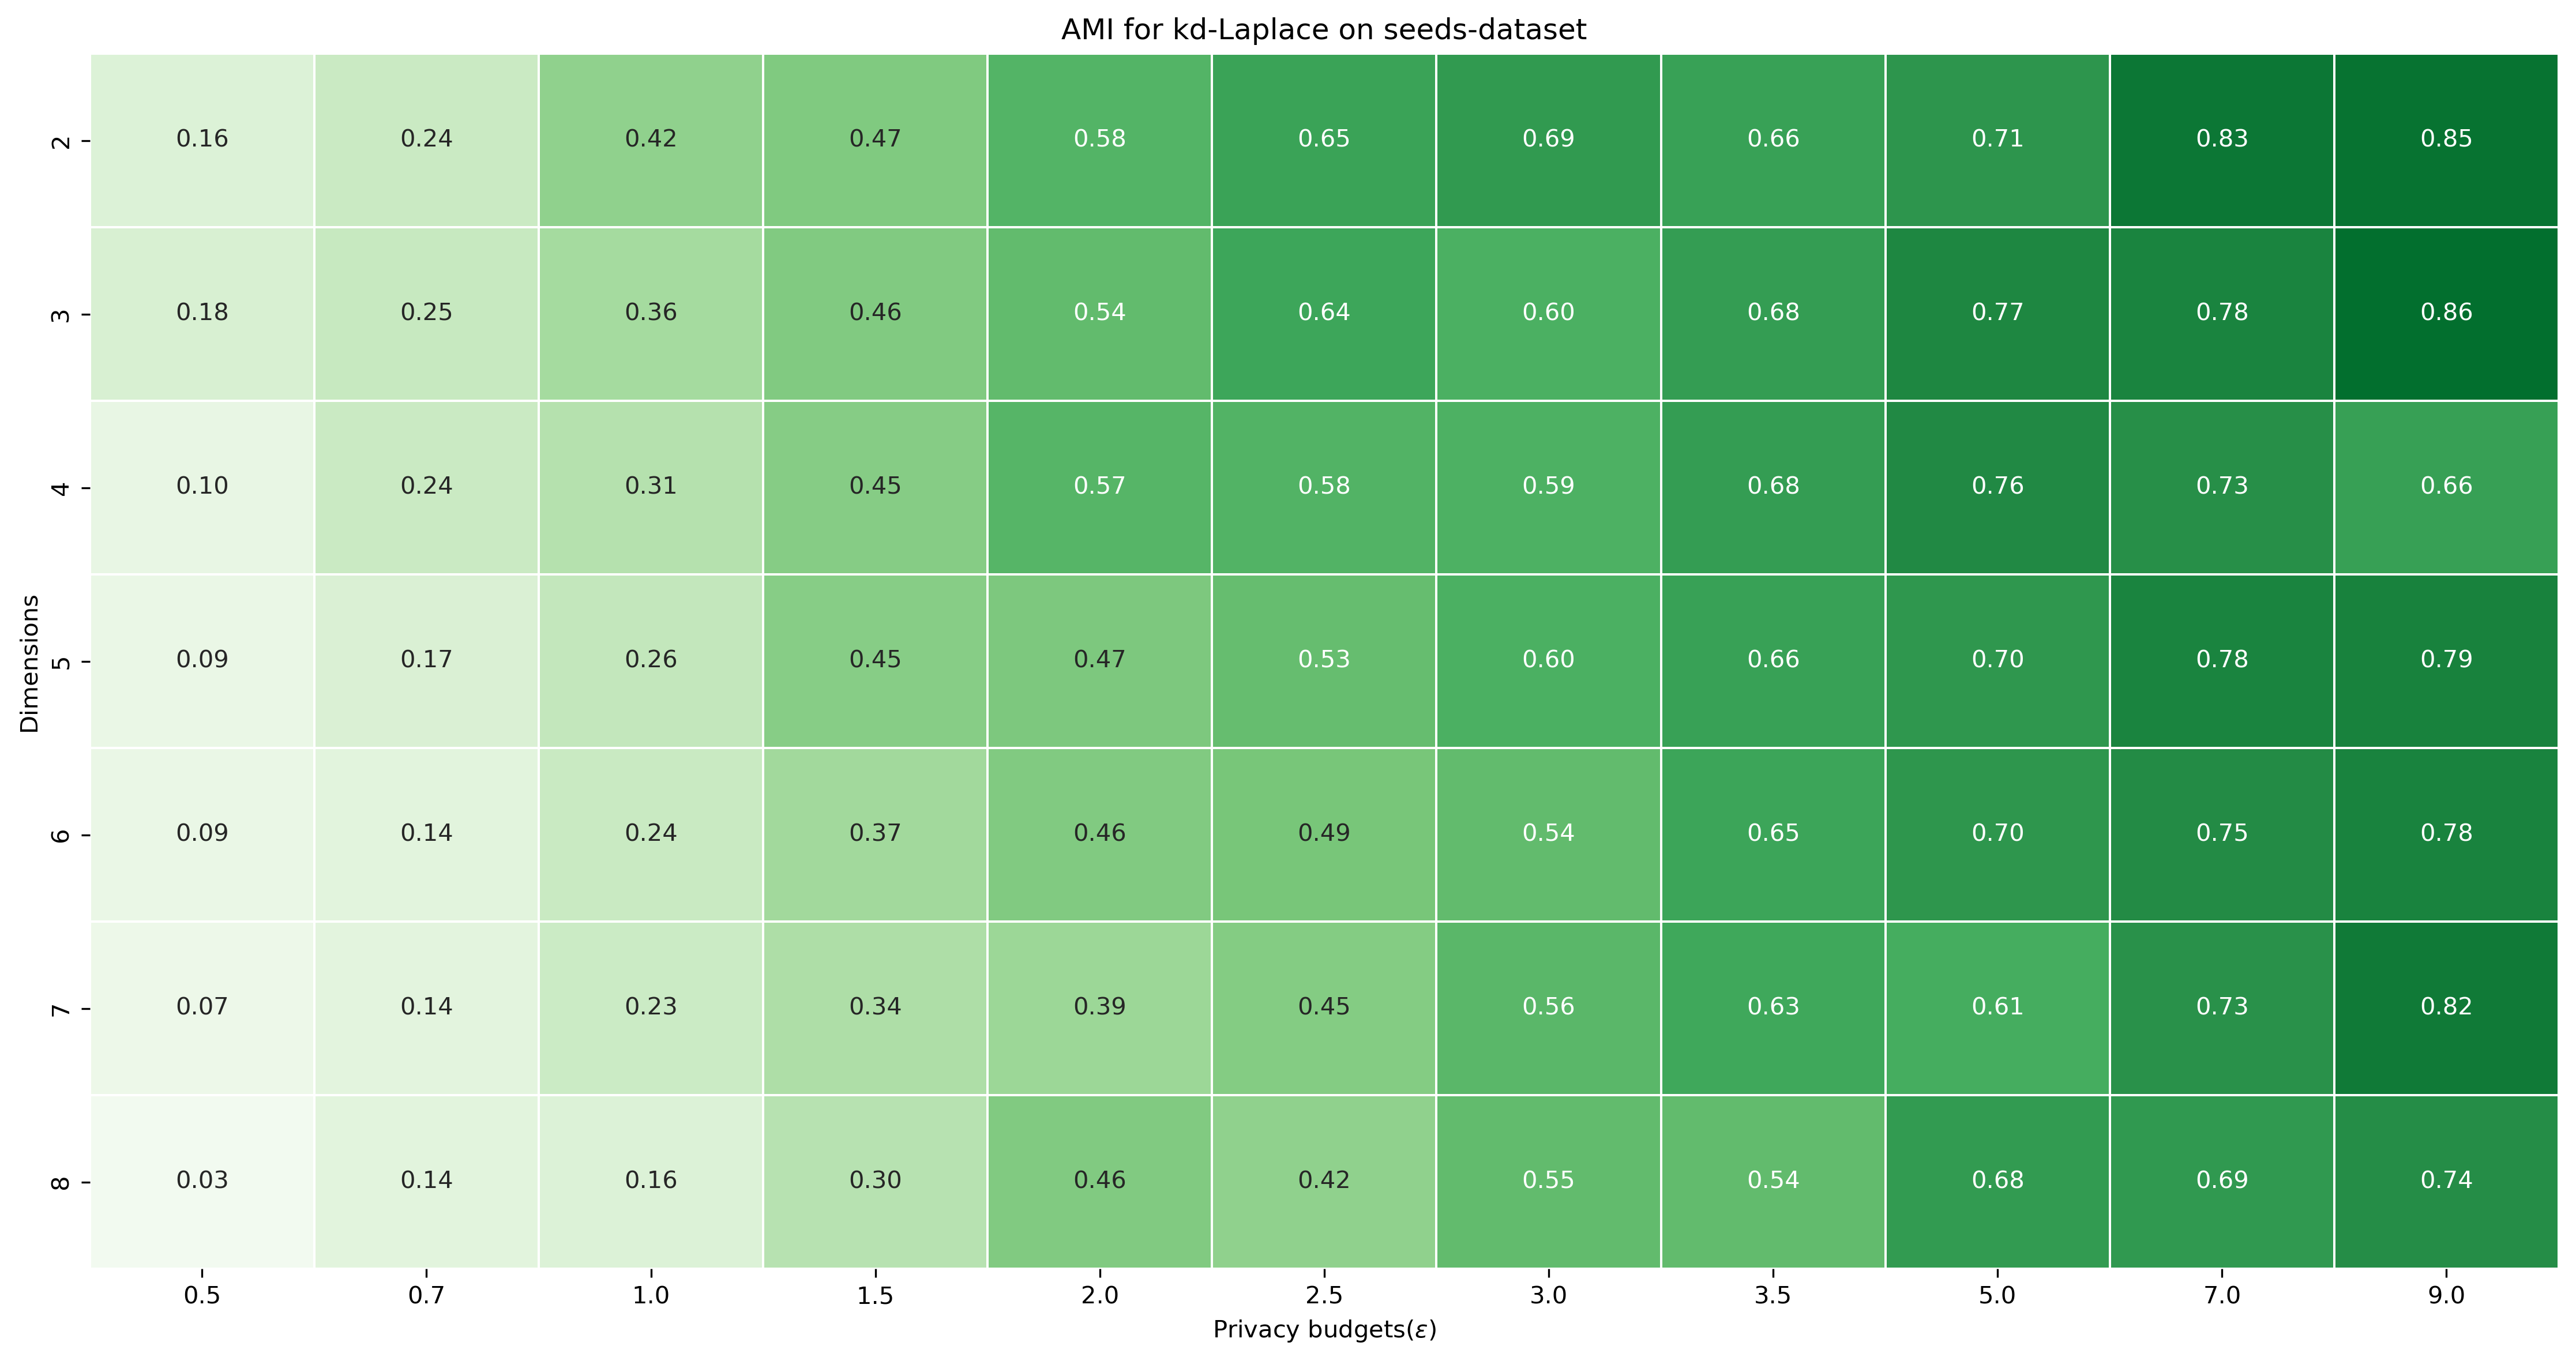
\includegraphics[width=1\textwidth]{Results/kd-laplace/kd-Laplace/seeds-dataset/ami.png}
                  \label{fig:ami_seeds-dataset_comparison_kdlaplace_2d}
            \end{subfigure}
            \vfill % vertical space
            \begin{subfigure}[c]{1\textwidth}
                  \caption{\textbf{Adjusted Mutual Information comparison for the Piecewise mechanism}}
                  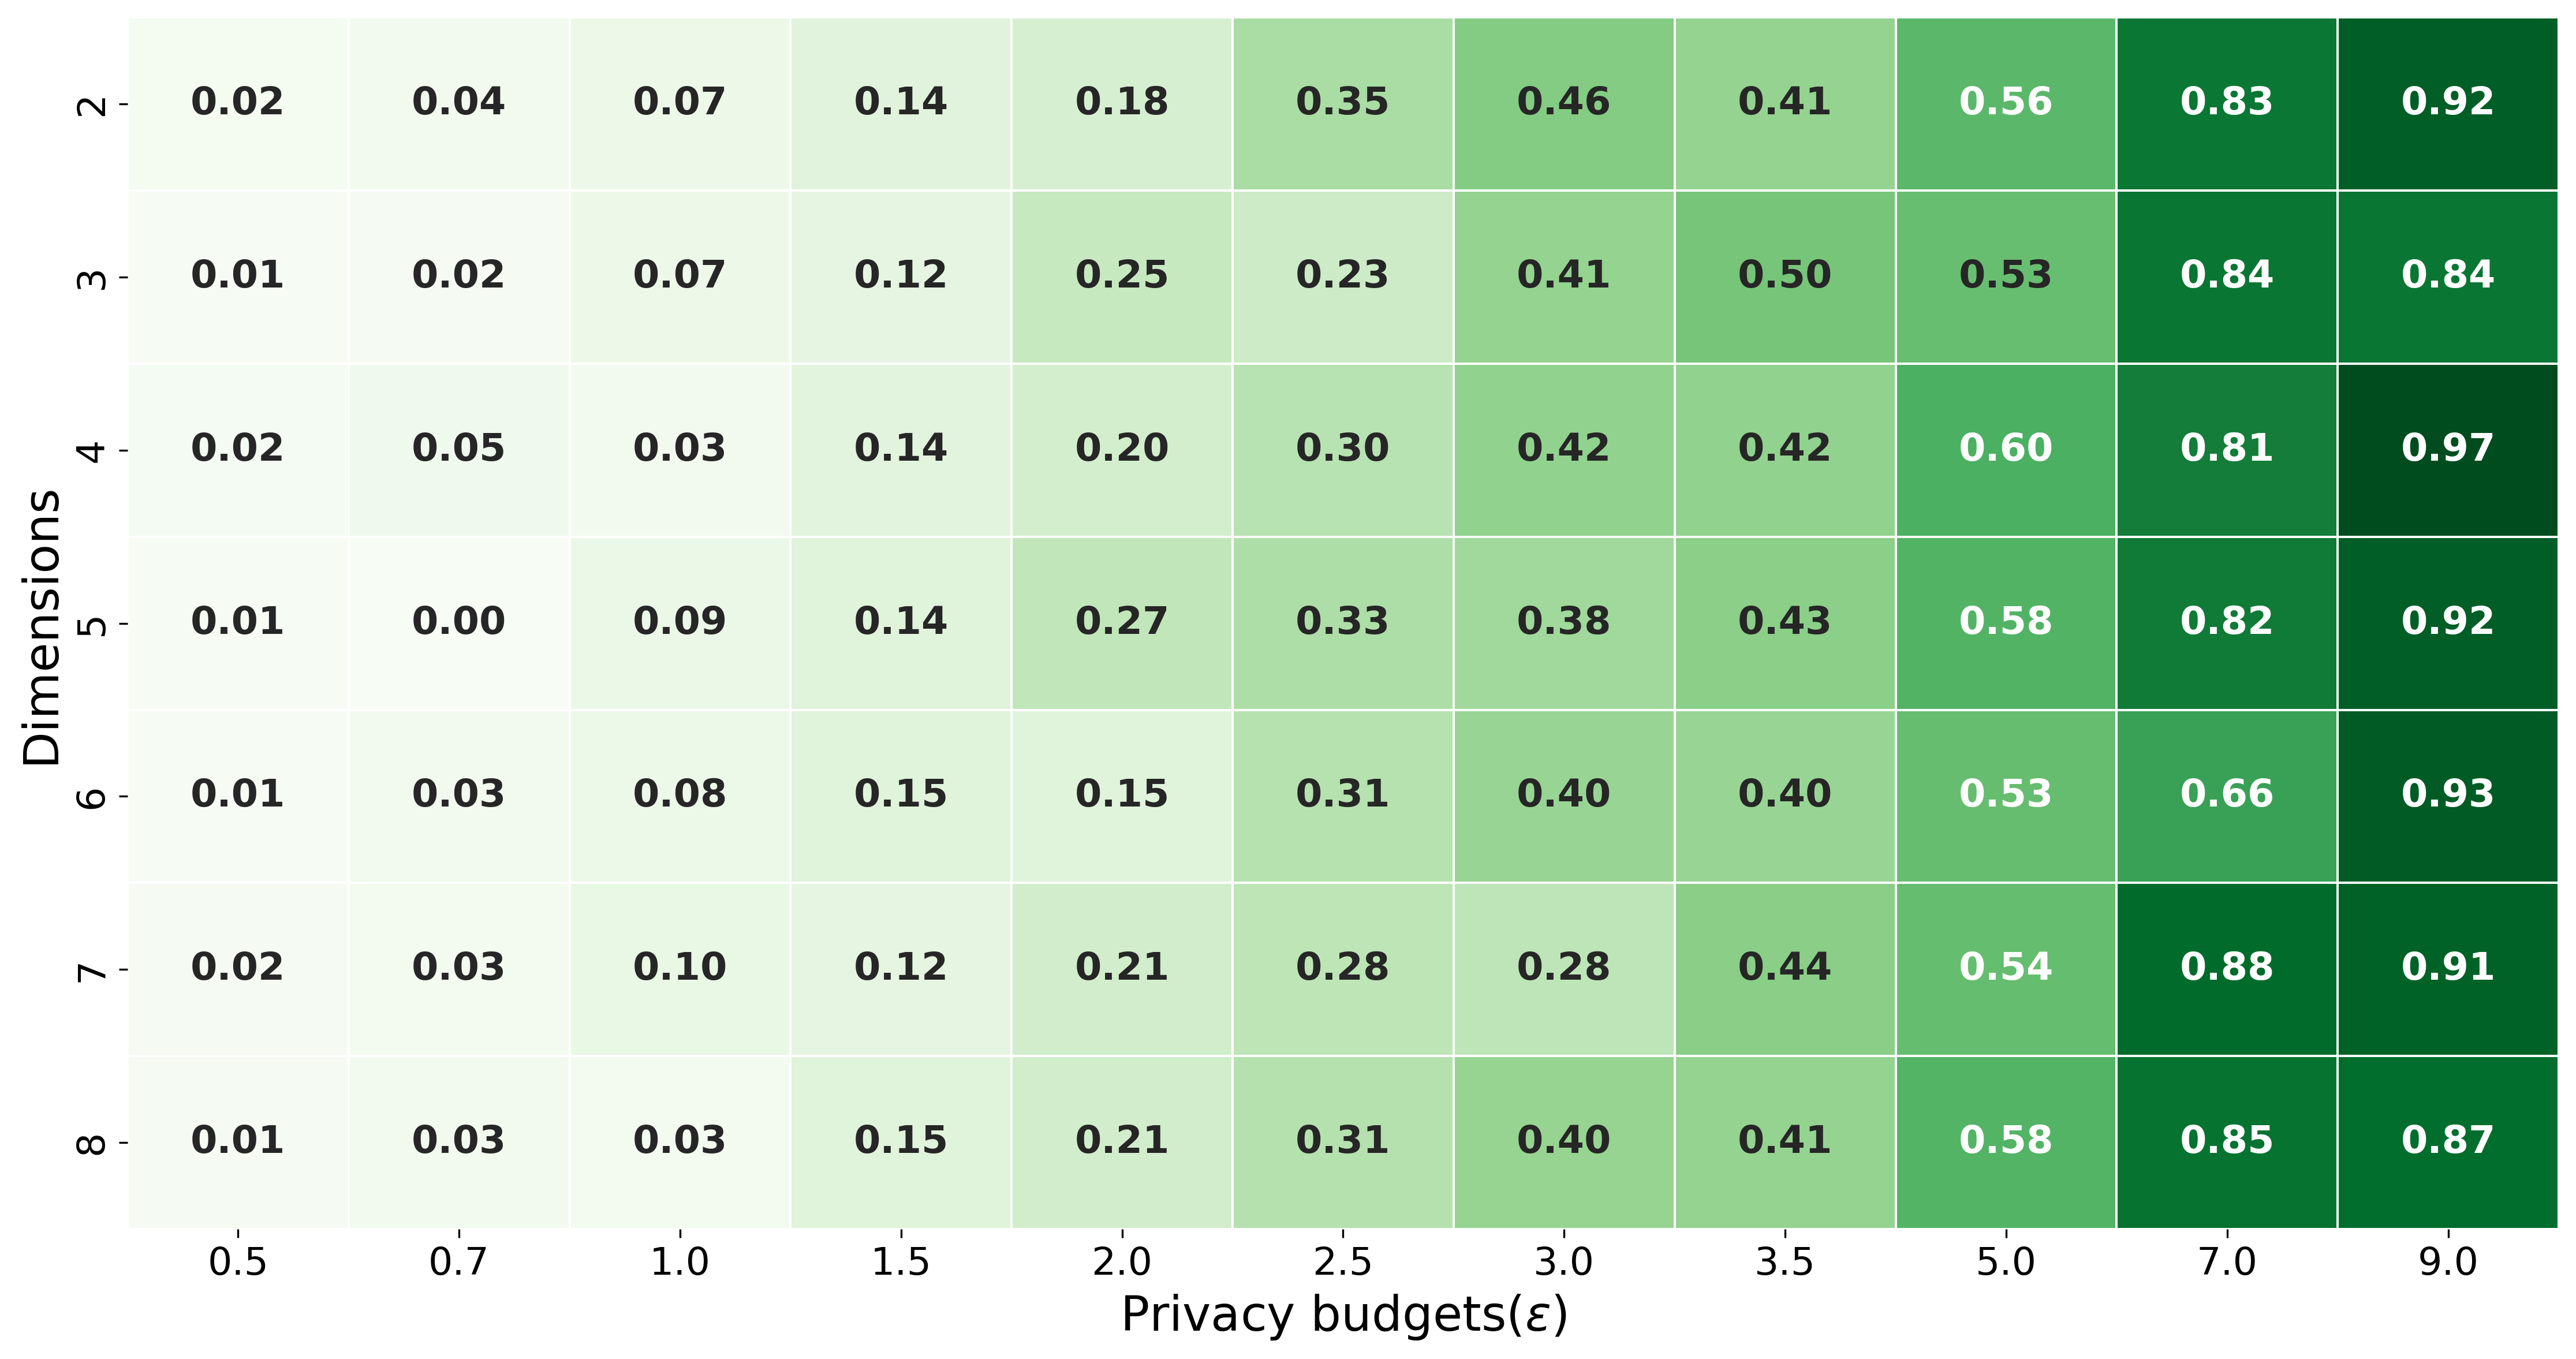
\includegraphics[width=1\textwidth]{Results/kd-laplace/piecewise/seeds-dataset/ami.png}
                  \label{fig:ami_seeds-dataset_comparison_piecewise_2d}
            \end{subfigure}
      \end{subfigure}
      \hfill % horizontal space
      \begin{subfigure}[b]{0.075\textwidth}
            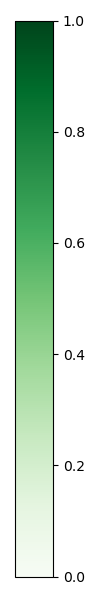
\includegraphics[width=1\textwidth]{Results/kd-laplace/kd-Laplace/seeds-dataset/heatmap_legend.png}
      \end{subfigure}
\end{figure}
The two plots compare external validation (\gls{ami}) between the two privacy mechanisms.
The kd-Laplace mechanism scores better for all privacy budgets (epsilon) for K-Means, except for privacy budgets 7 and 9.
For epsilon 5, Piecewise is slightly better, but kD-Laplace scores better for 2 dimensions.
KD-Laplace scores low for 2 - 5 dimensions and epsilon 0.5 and 0.7.
However, Piecewise scores < 0.10 \gls{ami} for epsilons < 3 for all dimensions.
\newpage
\subsection{Heart-dataset}
\begin{figure}[H]
      \centering
      \begin{subfigure}[b]{0.90\textwidth}
            \begin{subfigure}[c]{1\textwidth}
                  \caption{\textbf{Adjusted Mutual Information comparison for the kd-Laplace mechanism}}
                  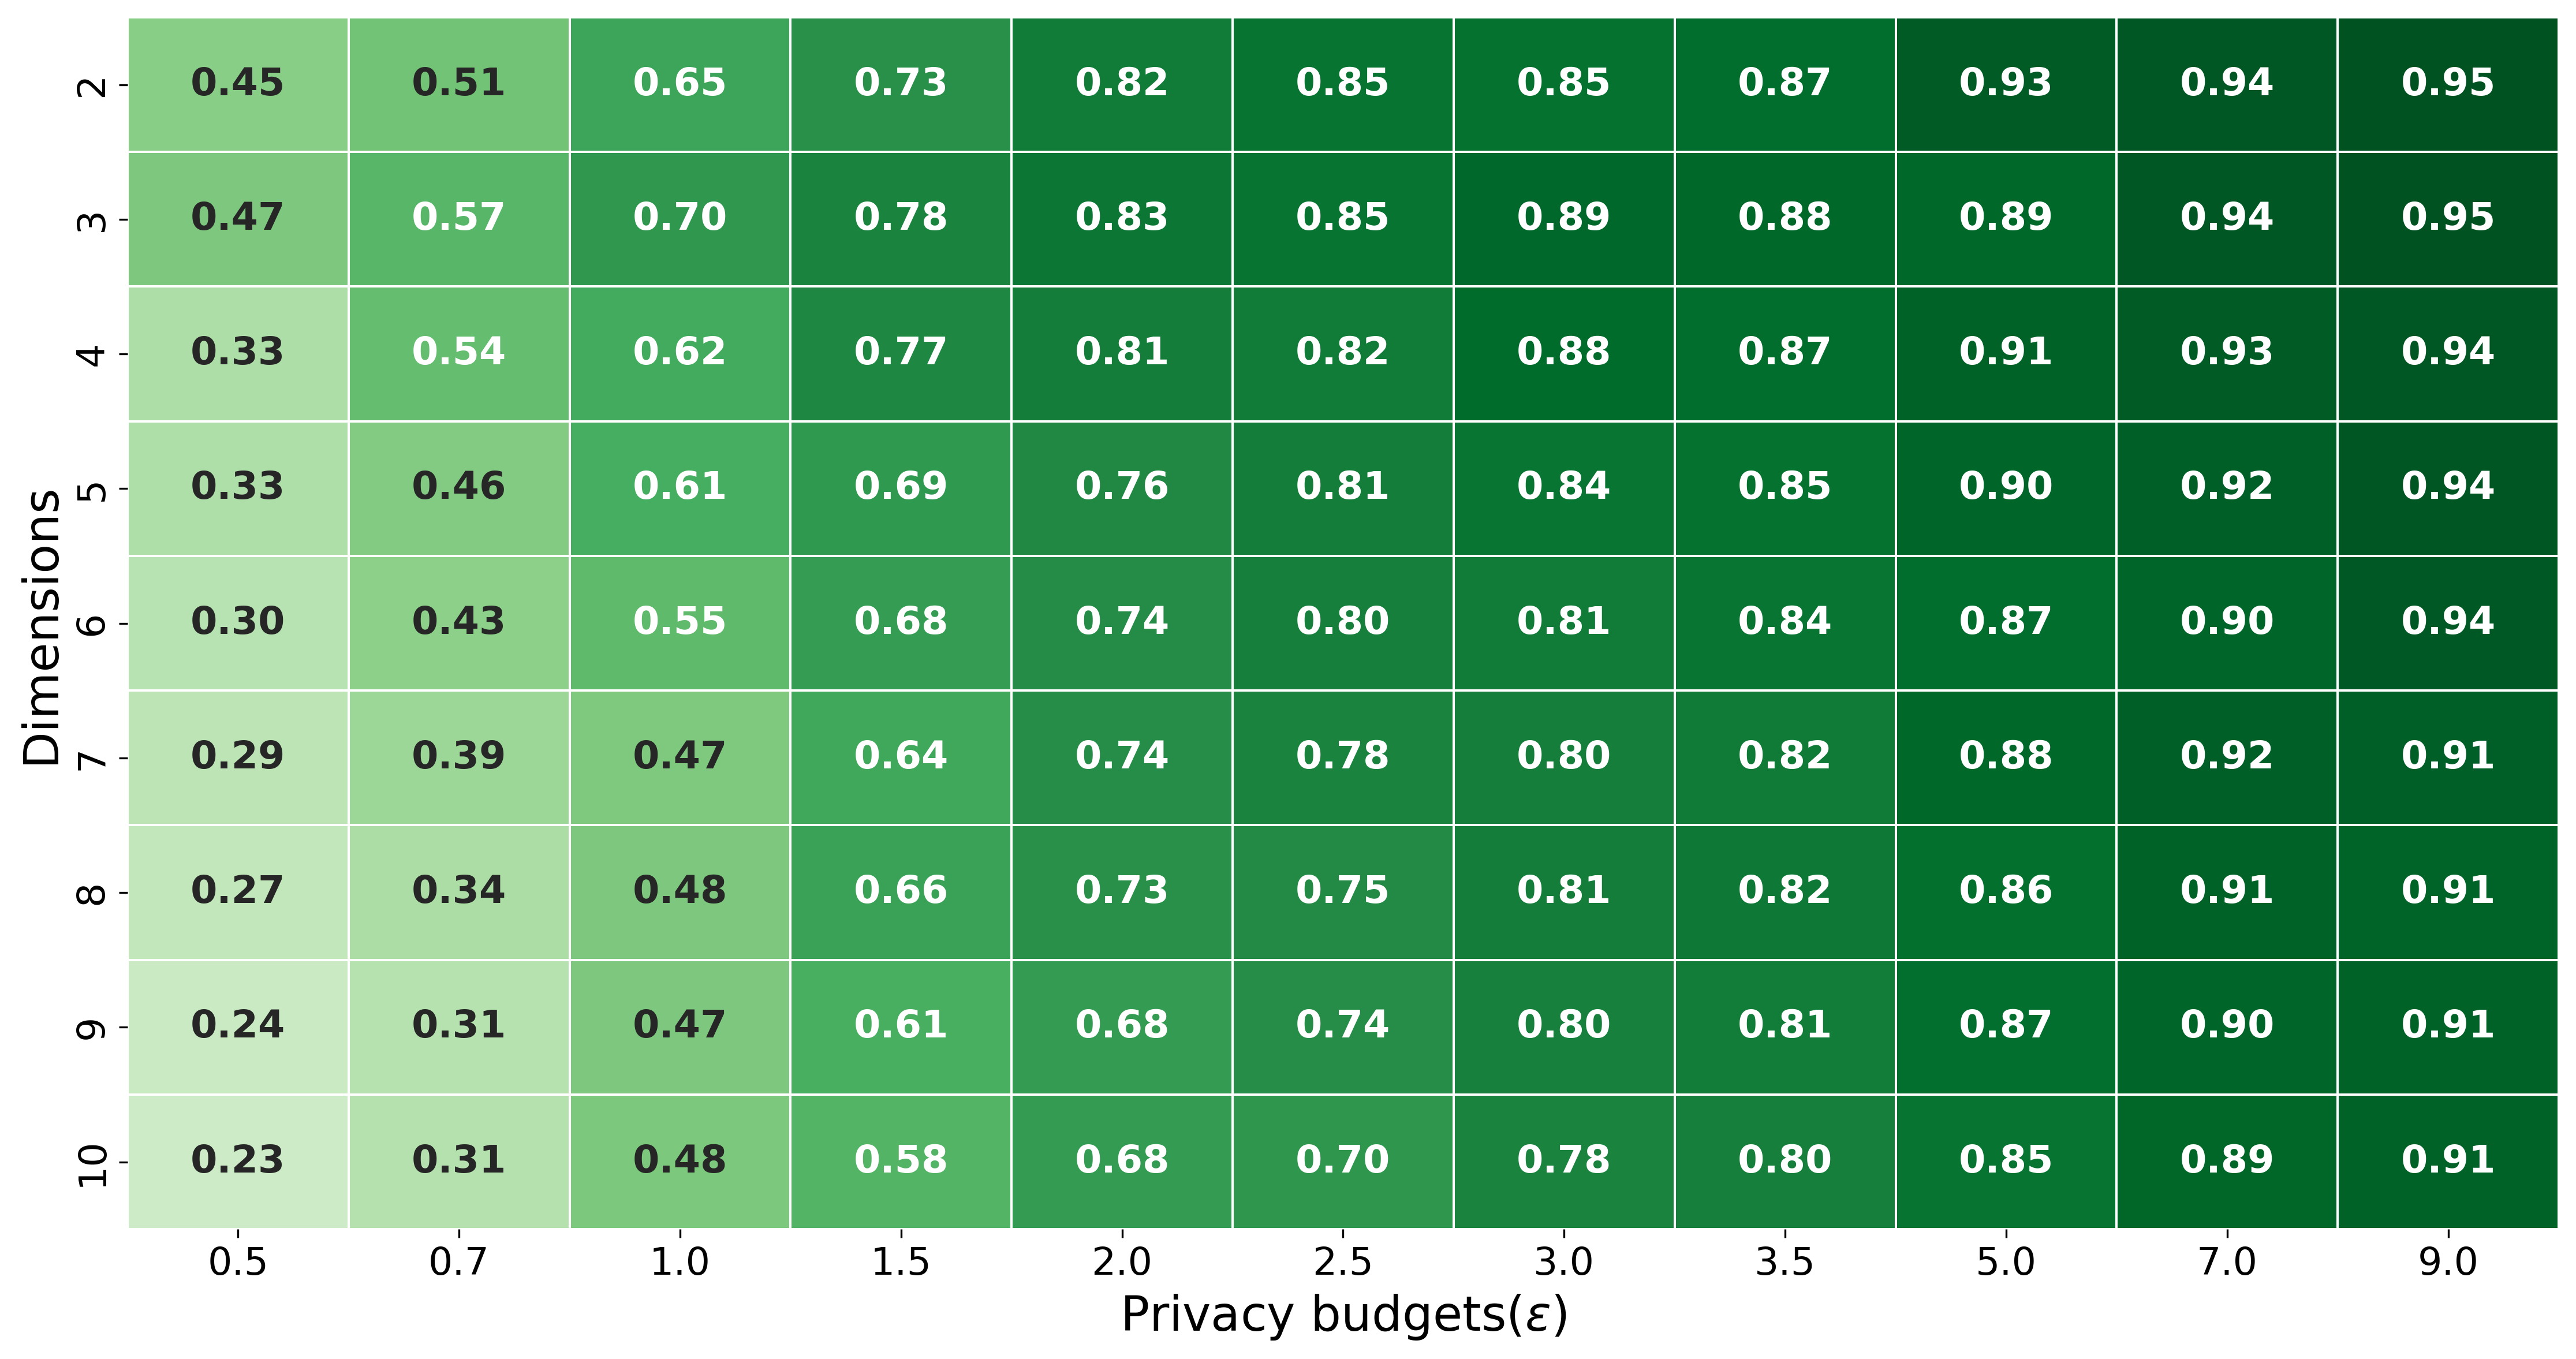
\includegraphics[width=1\textwidth]{Results/kd-laplace/kd-Laplace/heart-dataset/ami.png}
                  \label{fig:ami_heart-dataset_comparison_kdlaplace_2d}
            \end{subfigure}
            \vfill % vertical space
            \begin{subfigure}[c]{1\textwidth}
                  \caption{\textbf{Adjusted Mutual Information comparison for the Piecewise mechanism}}
                  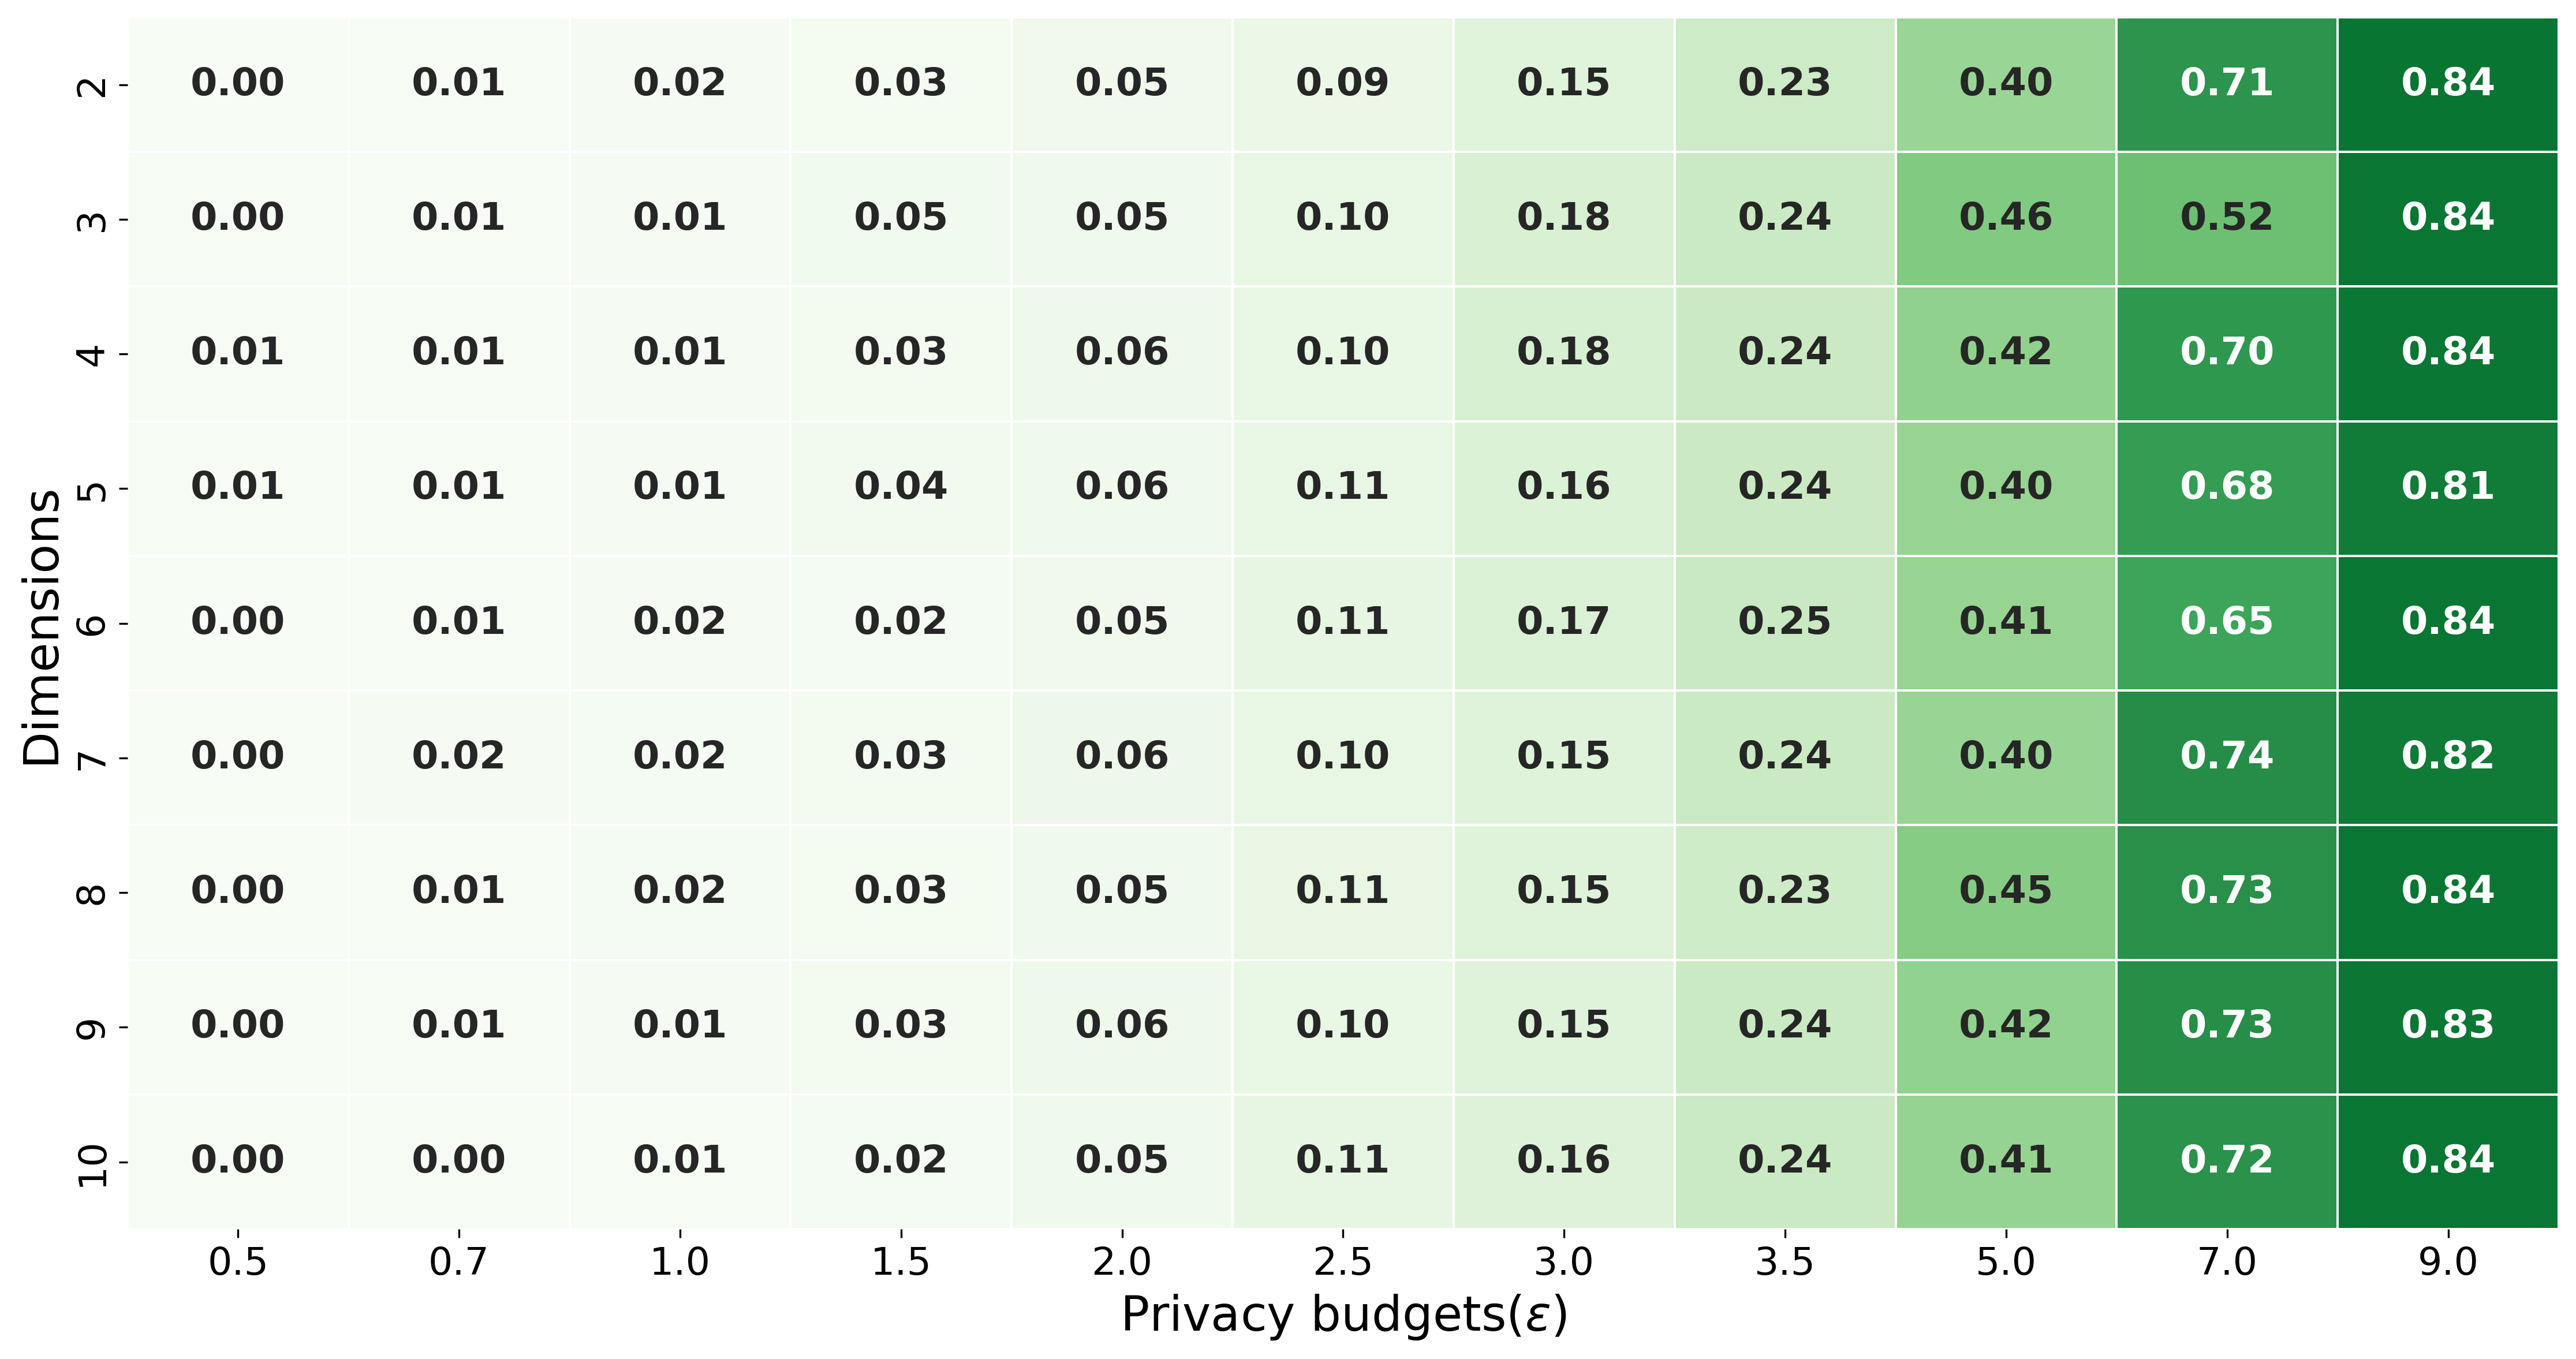
\includegraphics[width=1\textwidth]{Results/kd-laplace/piecewise/heart-dataset/ami.png}
                  \label{fig:ami_heart-dataset_comparison_piecewise_2d}
            \end{subfigure}
      \end{subfigure}
      \hfill % horizontal space
      \begin{subfigure}[b]{0.075\textwidth}
            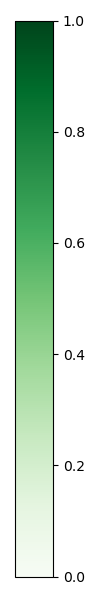
\includegraphics[width=1\textwidth]{Results/kd-laplace/kd-Laplace/seeds-dataset/heatmap_legend.png}
      \end{subfigure}
\end{figure}
For kD-Laplace, all scores are higher than 0.23 \gls{ami}.
Dimensions from 4 to 10 with a privacy budget of 0.5 have the lowest scores, but then the \gls{ami} increases.
Piecewise scores a maximum of 0.24 \gls{ami} for privacy budgets 0.5 to 3.5, with most values below 0.10. The number of dimensions does not seem to have an influence here.
The values for privacy budgets 7 and 9 are approximately 0.70 and 0.80 \gls{ami}, respectively.
\newpage
\subsection{Circle-dataset}
\begin{figure}[H]
      \centering
      \begin{subfigure}[b]{0.85\textwidth}
            \begin{subfigure}[c]{1\textwidth}
                  \caption{\textbf{Adjusted Mutual Information comparison for the kd-Laplace mechanism}}
                  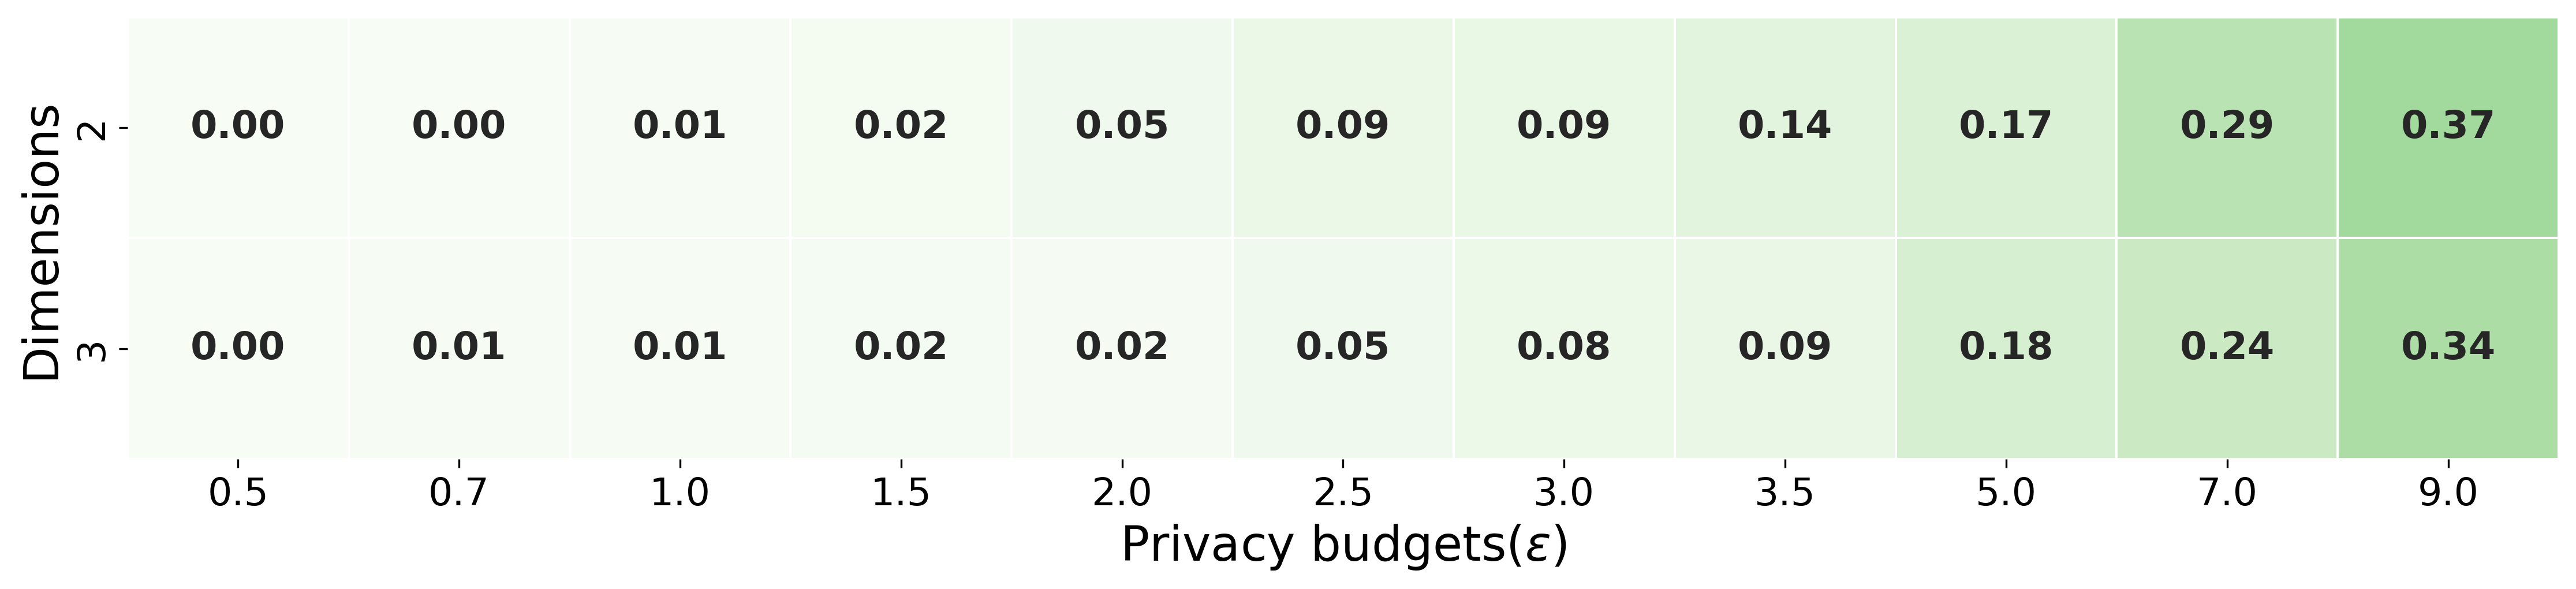
\includegraphics[width=1\textwidth]{Results/kd-laplace/kd-Laplace/circle-dataset/ami.png}
                  \label{fig:ami_circle-dataset_comparison_kdlaplace_2d}
            \end{subfigure}
            \vfill % vertical space
            \begin{subfigure}[c]{1\textwidth}
                  \caption{\textbf{Adjusted Mutual Information comparison for the Piecewise mechanism}}
                  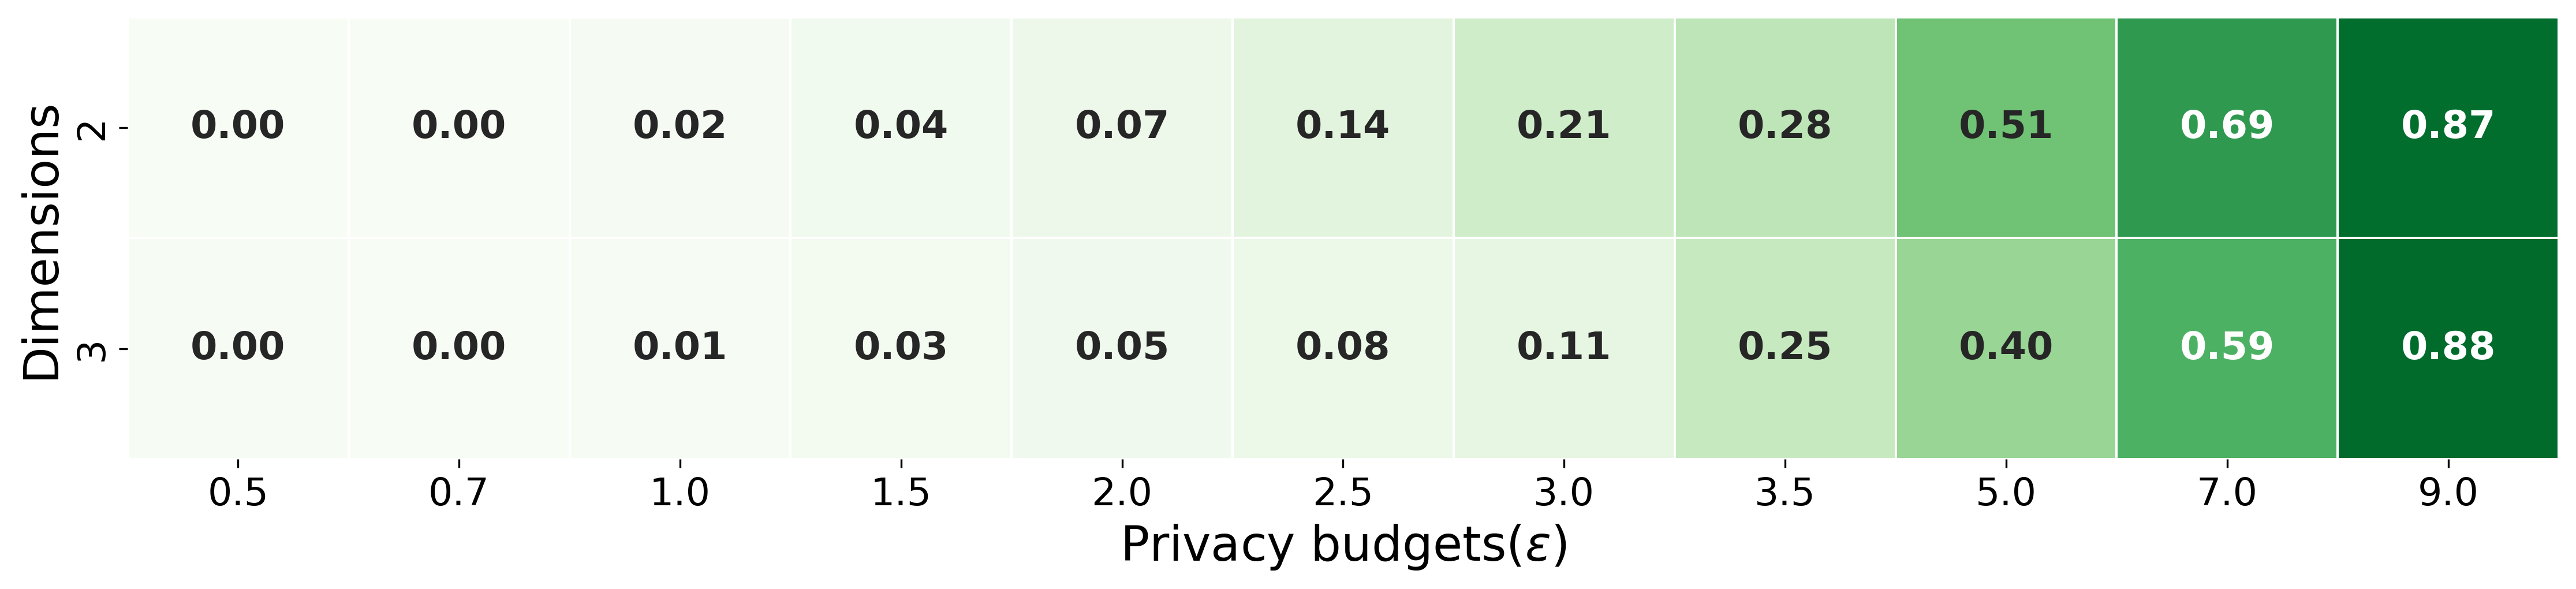
\includegraphics[width=1\textwidth]{Results/kd-laplace/piecewise/circle-dataset/ami.png}
                  \label{fig:ami_circle-dataset_comparison_piecewise_2d}
            \end{subfigure}
      \end{subfigure}
      \hfill % horizontal space
      \begin{subfigure}[b]{0.075\textwidth}
            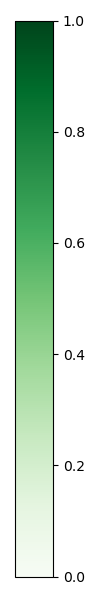
\includegraphics[width=1\textwidth]{Results/kd-laplace/kd-Laplace/seeds-dataset/heatmap_legend.png}
      \end{subfigure}
\end{figure}
kD-Laplace achieves the highest value of 0.37 \gls{ami} for privacy budget 9. However, the score remains low for the other privacy budgets, regardless of the dimension.
For Piecewise, the highest score is significantly higher, reaching a maximum of 0.88 \gls{ami} for privacy budget 9. The dimension does not seem to have much impact here, either.
\newpage
\subsection{Line-dataset}
\begin{figure}[H]
      \centering
      \begin{subfigure}[b]{0.85\textwidth}
            \begin{subfigure}[c]{1\textwidth}
                  \caption{\textbf{Adjusted Mutual Information comparison for the kd-Laplace mechanism}}
                  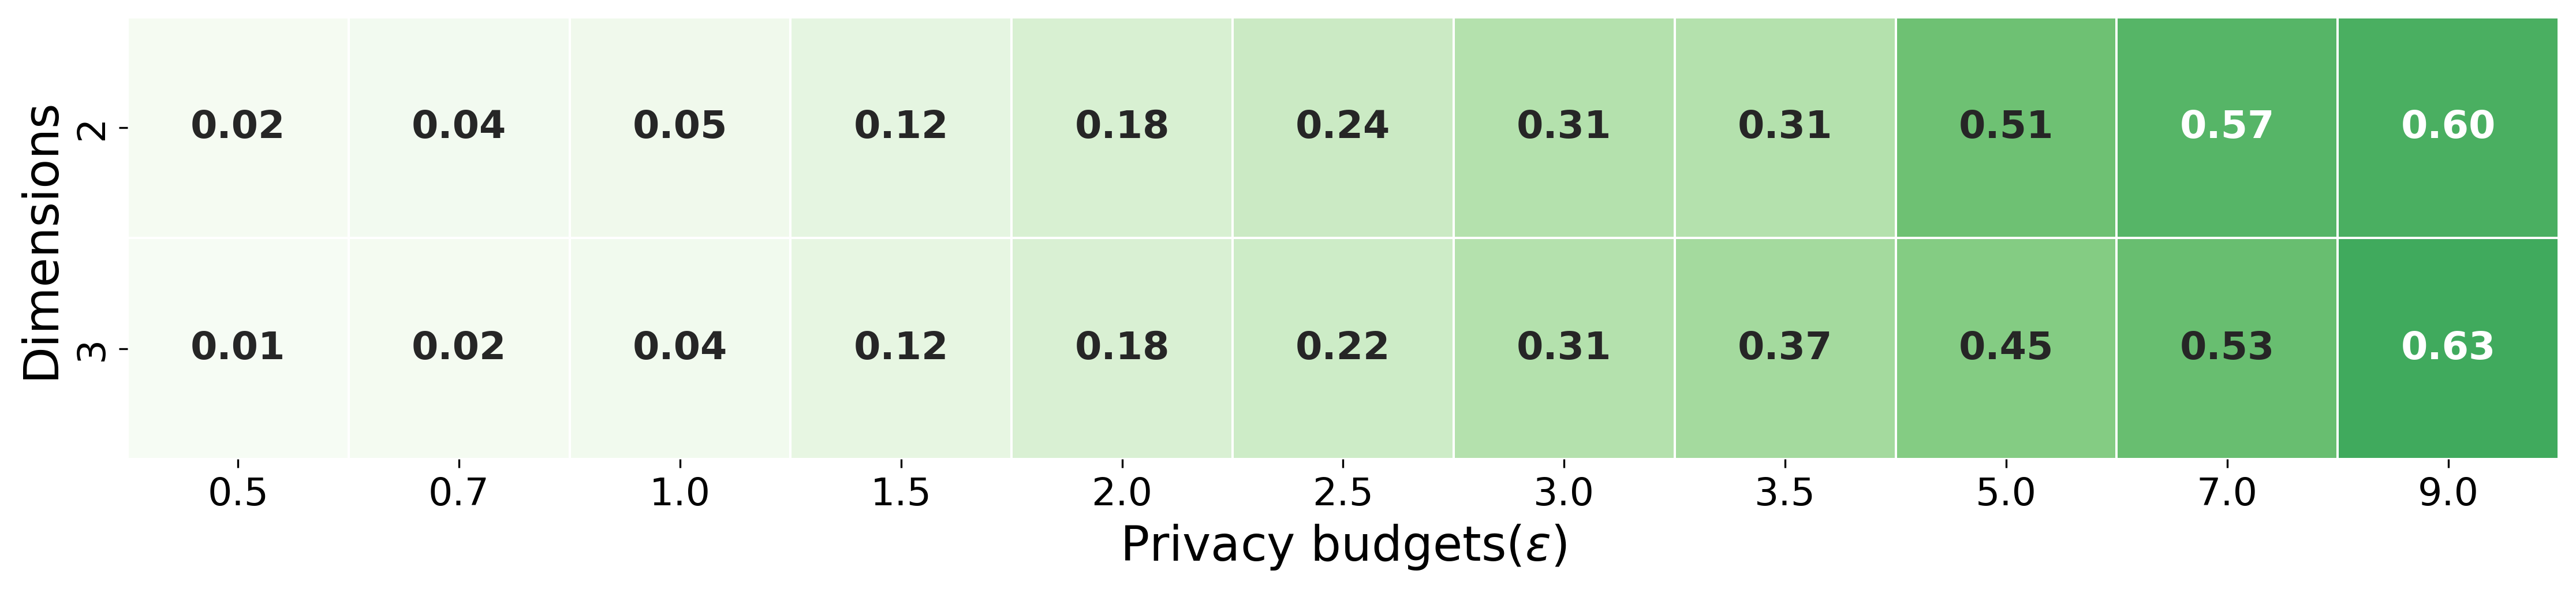
\includegraphics[width=1\textwidth]{Results/kd-laplace/kd-Laplace/line-dataset/ami.png}
                  \label{fig:ami_line-dataset_comparison_kdlaplace_2d}
            \end{subfigure}
            \vfill % vertical space
            \begin{subfigure}[c]{1\textwidth}
                  \caption{\textbf{Adjusted Mutual Information comparison for the Piecewise mechanism}}
                  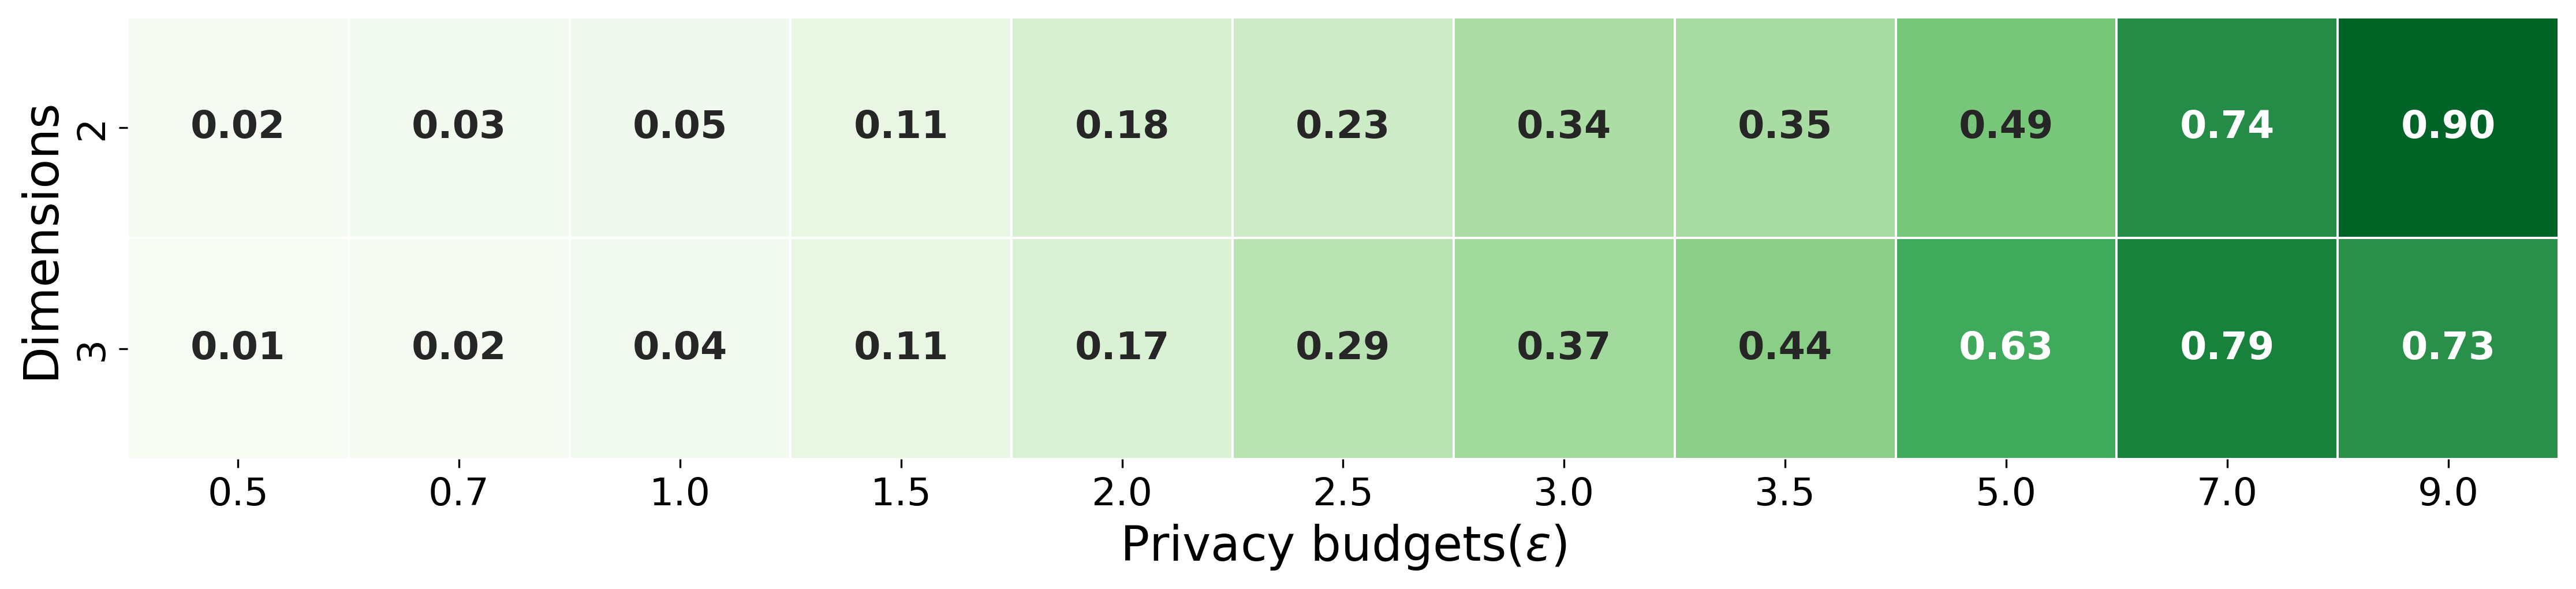
\includegraphics[width=1\textwidth]{Results/kd-laplace/piecewise/line-dataset/ami.png}
                  \label{fig:ami_line-dataset_comparison_piecewise_2d}
            \end{subfigure}
      \end{subfigure}
      \hfill % horizontal space
      \begin{subfigure}[b]{0.075\textwidth}
            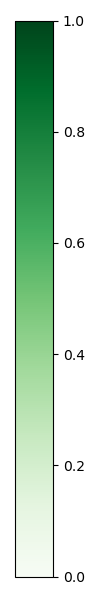
\includegraphics[width=1\textwidth]{Results/kd-laplace/kd-Laplace/seeds-dataset/heatmap_legend.png}
      \end{subfigure}
\end{figure}
Up to privacy budget 3.5, the scores remain relatively similar for both mechanisms, but after that, they become better for Piecewise.

For kD-Laplace, the highest score is 0.63 \gls{ami} for privacy budget 9. For privacy budgets 5 and 7, the score is around 0.5 - 0.55. After that, the scores are no higher than 0.37.

Piecewise performs better, with a maximum of 0.90 \gls{ami} for privacy budget 9 for 2 dimensions. For both mechanisms, the dimensions do not significantly impact the score.
\newpage
\subsection{Skewed-dataset}
\begin{figure}[H]
      \centering
      \begin{subfigure}[b]{0.85\textwidth}
            \begin{subfigure}[c]{1\textwidth}
                  \caption{\textbf{Adjusted Mutual Information comparison for the kd-Laplace mechanism}}
                  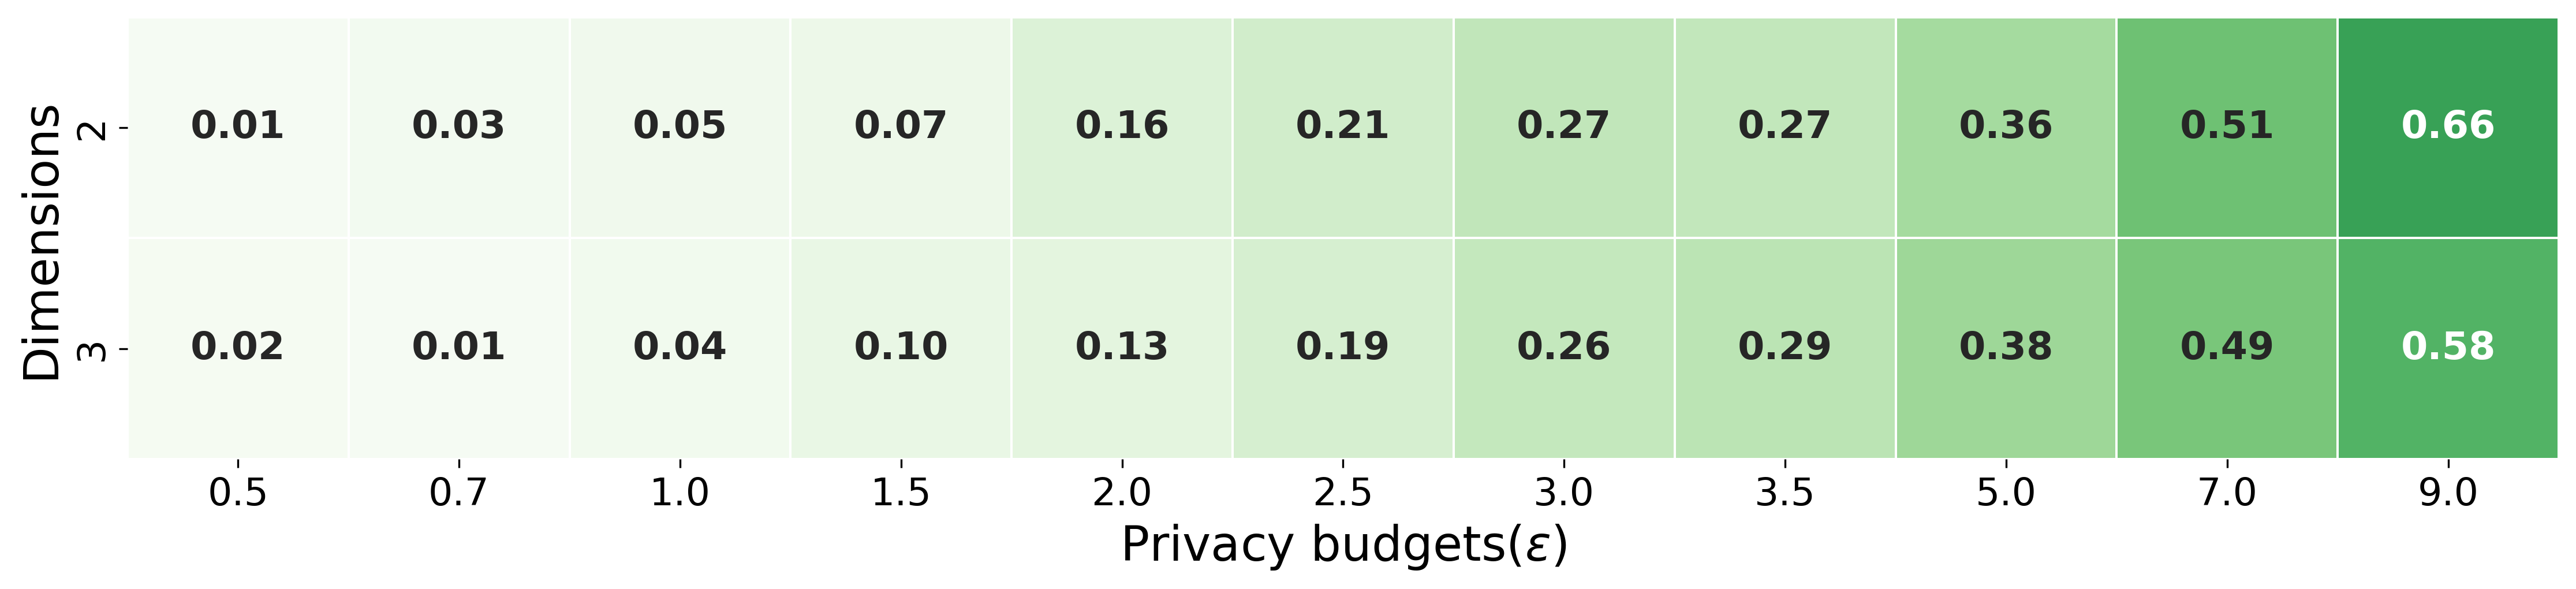
\includegraphics[width=1\textwidth]{Results/kd-laplace/kd-Laplace/skewed-dataset/ami.png}
                  \label{fig:ami_skewed-dataset_comparison_kdlaplace_2d}
            \end{subfigure}
            \vfill % vertical space
            \begin{subfigure}[c]{1\textwidth}
                  \caption{\textbf{Adjusted Mutual Information comparison for the Piecewise mechanism}}
                  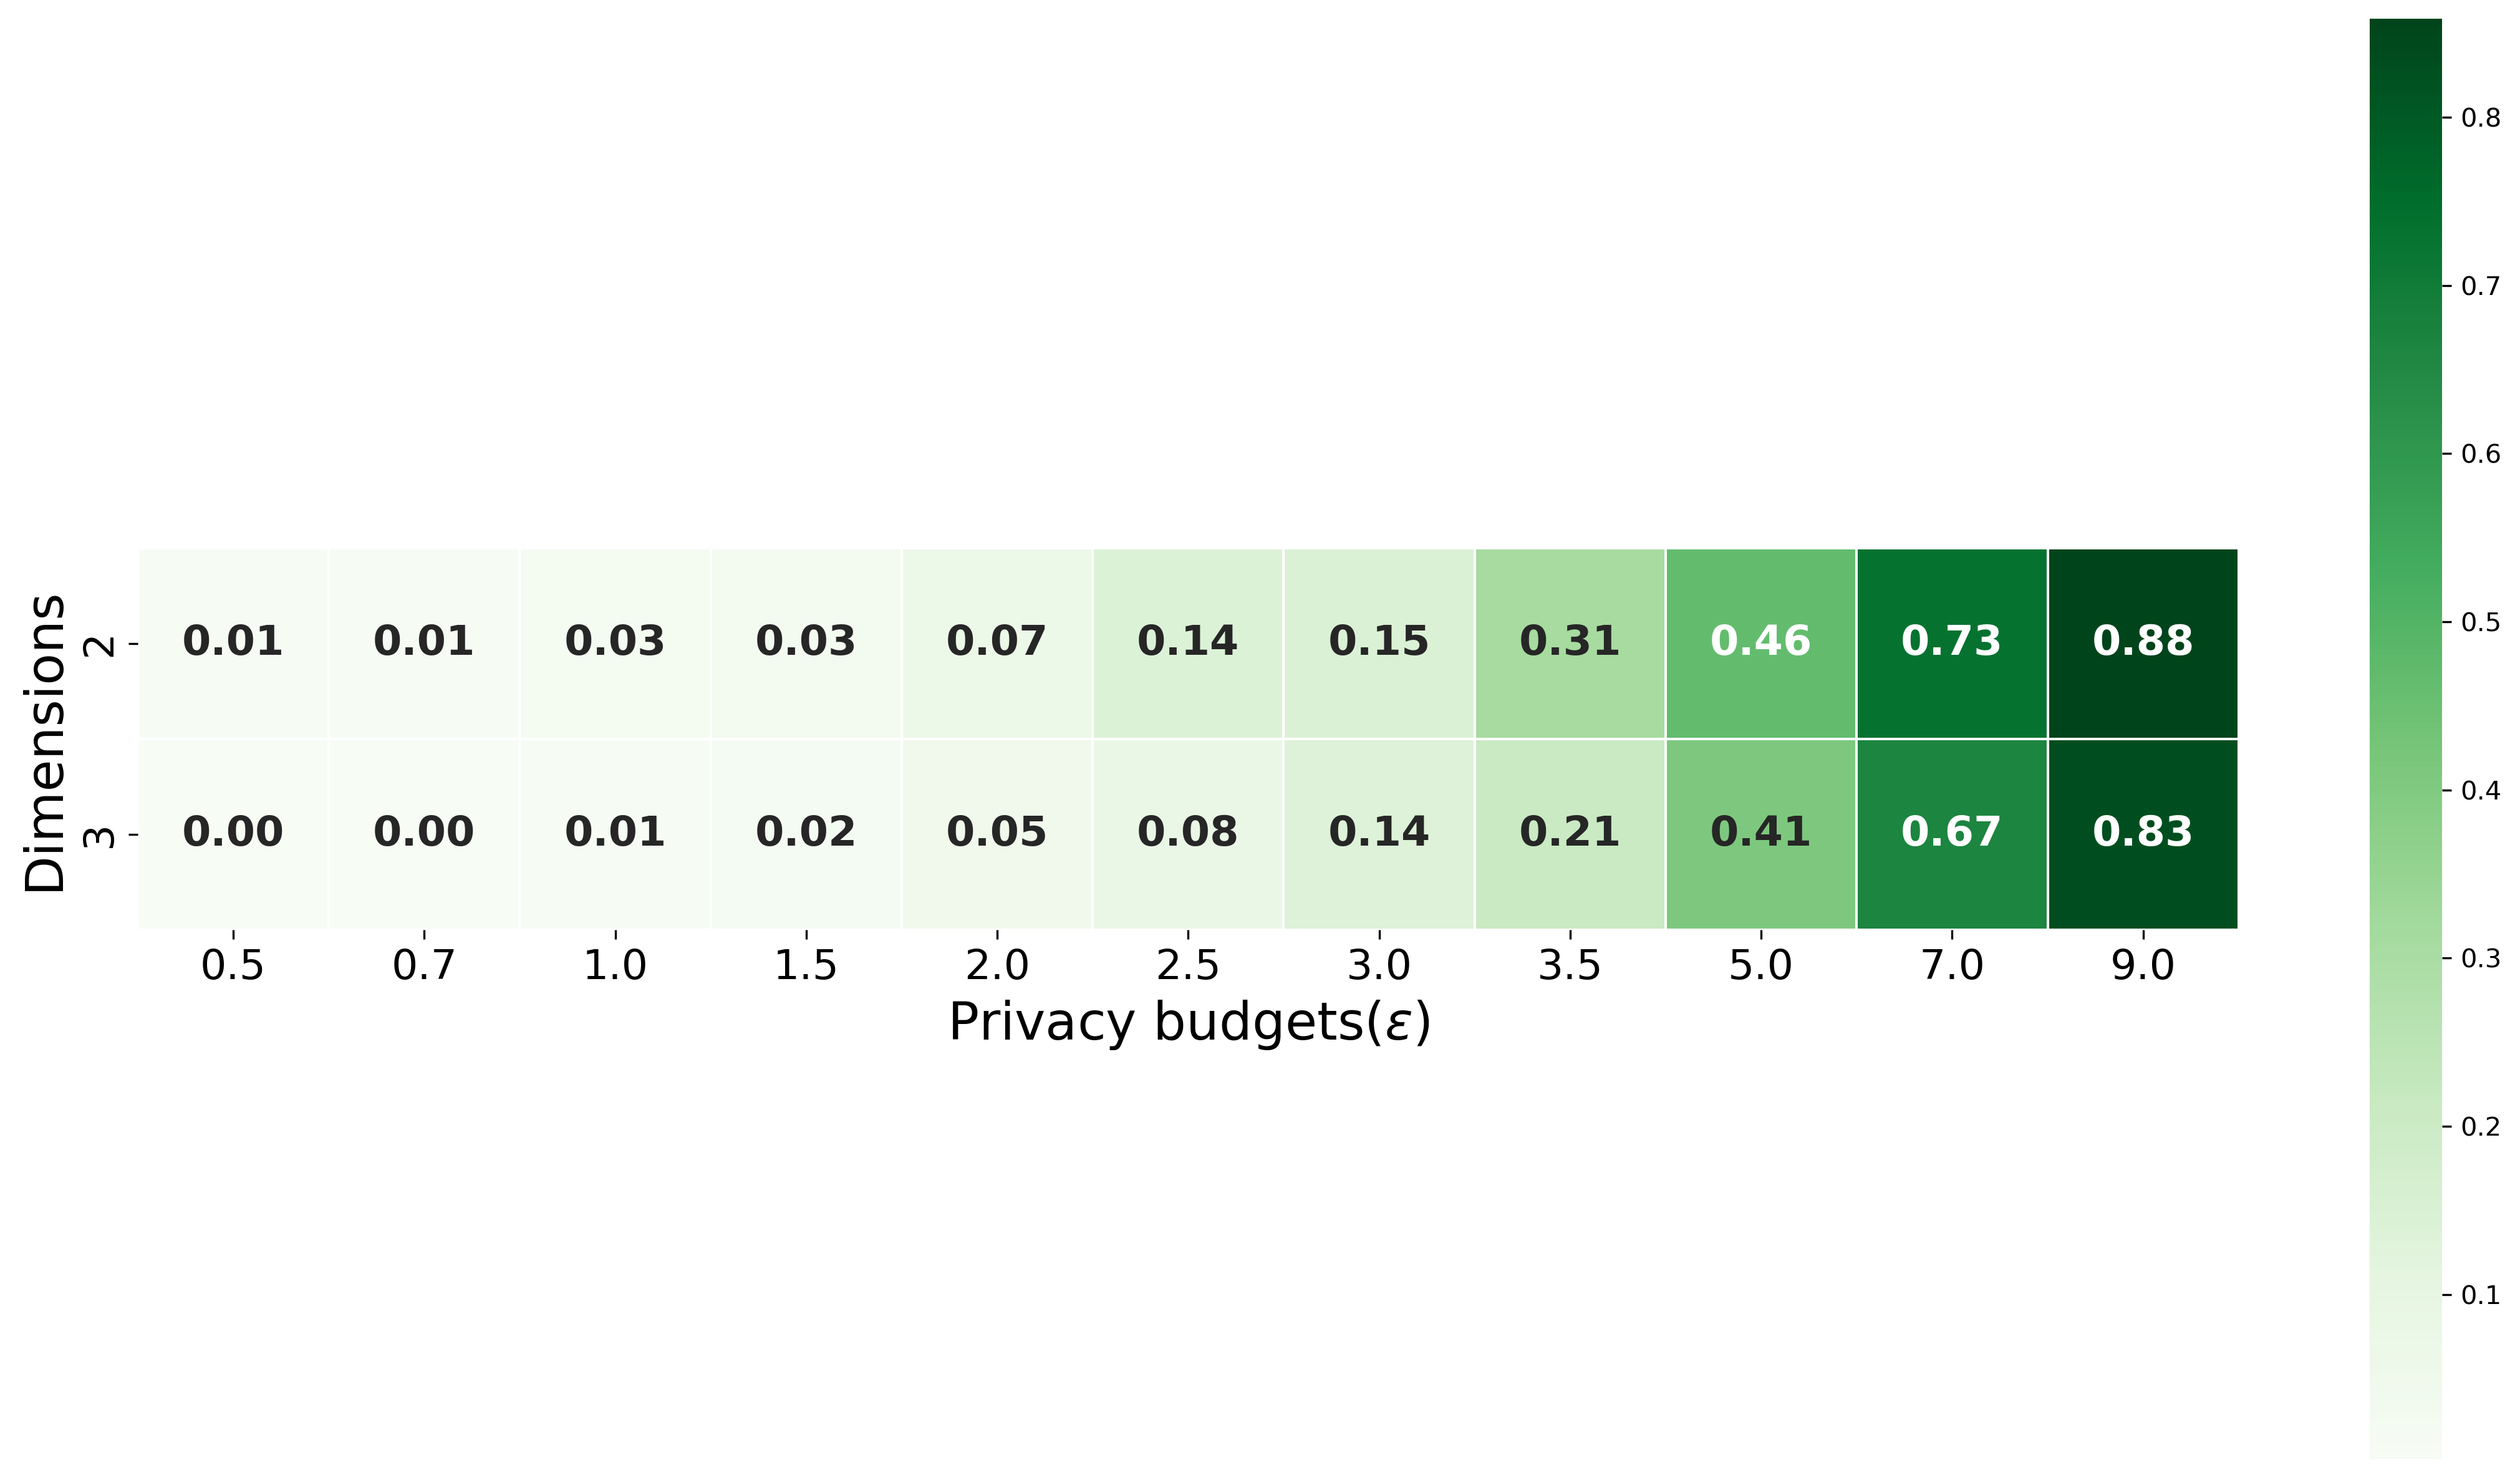
\includegraphics[width=1\textwidth]{Results/kd-laplace/piecewise/skewed-dataset/ami.png}
                  \label{fig:ami_skewed-dataset_comparison_piecewise_2d}
            \end{subfigure}
      \end{subfigure}
      \hfill % horizontal space
      \begin{subfigure}[b]{0.075\textwidth}
            \includegraphics[width=1\textwidth]{Results/kd-laplace/kd-Laplace/skewed-dataset/heatmap_legend_ami.png}
      \end{subfigure}
\end{figure}
The kD-Laplace mechanism performs slightly better from privacy budgets 2 to 5. However, Piecewise performs significantly better after that, achieving around 0.73 and 0.85 \gls{ami} for privacy budgets 7 and 9, respectively.

In contrast, kD-Laplace scores much lower in this range. Furthermore, it appears that the dimensions do not significantly impact the performance of the mechanisms in this context.
\newpage
\section{Privacy}
%The images below display bar plots for the membership advantage and TPR of membership inference attacks as described in the methodology.
%We use the same color scheme in the previous section to display the different mechanisms.
%In addition, a red line was drawn to indicate the baseline TPR (the non-private dataset's TPR). \newline
\subsection{Seeds dataset}
\begin{figure}[H]
      \centering
      \begin{subfigure}[b]{0.9\textwidth}
            \begin{subfigure}[c]{1\textwidth}
                  \caption{\textbf{Heatmap showing adversary advantage for the kD-Laplace mechanism, per privacy budget \& dimension for seeds-dataset.}}
                  \includegraphics[width=1\textwidth]{Results/kd-laplace/kd-Laplace/seeds-dataset/shokri_mi_adv.png}
                  \label{fig:privacy_seeds-dataset_adversial_advantage_kd-laplace}
            \end{subfigure}
            \vfill % vertical space

            \begin{subfigure}[c]{1\textwidth}
                  \caption{\textbf{Heatmap showing adversary advantage for the Piecewise mechanism, per privacy budget \& dimension for seeds-dataset.}}
                  \includegraphics[width=1\textwidth]{Results/kd-laplace/piecewise/seeds-dataset/shokri_mi_adv.png}
                  \label{fig:privacy_seeds-dataset_adversial_advantage_piecewise}
            \end{subfigure}
      \end{subfigure}
      \hfill % horizontal space
      \begin{subfigure}[b]{0.075\textwidth}
            \includegraphics[width=1\textwidth]{Results/kd-laplace/kd-Laplace/seeds-dataset/heatmap_legend_shokri_mi_adv.png}
      \end{subfigure}
\end{figure}
The heatmaps show the adversary advantage of kD-Laplace and Piecewise mechanisms.
For kD-Laplace, the advantage slightly decreases with higher privacy budgets.
Dimension 4 has a relatively high advantage for budgets 0.5 and 0.7. Piecewise generally has a higher advantage, especially for 2 dimensions (around +/- 0.5).
Overall, dimensions don't have a significant impact on the advantage for both mechanisms.
\newpage
\subsection{Heart dataset}
\begin{figure}[H]
      \centering
      \begin{subfigure}[b]{0.85\textwidth}
            \begin{subfigure}[c]{1\textwidth}
                  \caption{\textbf{Heatmap showing adversary advantage for the kD-Laplace mechanism, per privacy budget \& dimension for heart-dataset.}}
                  \includegraphics[width=1\textwidth]{Results/kd-laplace/kd-Laplace/heart-dataset/shokri_mi_adv.png}
                  \label{fig:privacy_heart-dataset_adversial_advantage_kd-laplace}
            \end{subfigure}
            \vfill % vertical space

            \begin{subfigure}[c]{1\textwidth}
                  \caption{\textbf{Heatmap showing adversary advantage for the Piecewise mechanism, per privacy budget \& dimension for heart-dataset.}}
                  \includegraphics[width=1\textwidth]{Results/kd-laplace/piecewise/heart-dataset/shokri_mi_adv.png}
                  \label{fig:privacy_heart-dataset_adversial_advantage_piecewise}
            \end{subfigure}
      \end{subfigure}
      \hfill % horizontal space
      \begin{subfigure}[b]{0.075\textwidth}
            \includegraphics[width=1\textwidth]{Results/kd-laplace/kd-Laplace/heart-dataset/heatmap_legend_shokri_mi_adv.png}
      \end{subfigure}
\end{figure}

\newpage
\subsection{Circle dataset}
\begin{figure}[H]
      \centering
      \begin{subfigure}[b]{0.85\textwidth}
            \begin{subfigure}[c]{1\textwidth}
                  \caption{\textbf{Heatmap showing adversary advantage for the kD-Laplace mechanism, per privacy budget \& dimension for circle-dataset.}}
                  \includegraphics[width=1\textwidth]{Results/kd-laplace/kd-Laplace/circle-dataset/shokri_mi_adv.png}
                  \label{fig:privacy_circle-dataset_adversial_advantage_kd-laplace}
            \end{subfigure}
            \vfill % vertical space

            \begin{subfigure}[c]{1\textwidth}
                  \caption{\textbf{Heatmap showing adversary advantage for the Piecewise mechanism, per privacy budget \& dimension for seeds-dataset.}}
                  \includegraphics[width=1\textwidth]{Results/kd-laplace/piecewise/circle-dataset/shokri_mi_adv.png}
                  \label{fig:privacy_circle-dataset_adversial_advantage_piecewise}
            \end{subfigure}
      \end{subfigure}
      \hfill % horizontal space
      \begin{subfigure}[b]{0.075\textwidth}
            \includegraphics[width=1\textwidth]{Results/kd-laplace/kd-Laplace/circle-dataset/heatmap_legend_shokri_mi_adv.png}
      \end{subfigure}


\end{figure}

\newpage
\subsection{Line dataset}
\begin{figure}[H]
      \centering
      \begin{subfigure}[b]{0.85\textwidth}
            \begin{subfigure}[c]{1\textwidth}
                  \caption{\textbf{Heatmap showing adversary advantage for the kD-Laplace mechanism, per privacy budget \& dimension for seeds-dataset.}}
                  \includegraphics[width=1\textwidth]{Results/kd-laplace/kd-Laplace/line-dataset/shokri_mi_adv.png}
                  \label{fig:privacy_line-dataset_adversial_advantage_kd-laplace}
            \end{subfigure}
            \vfill % vertical space

            \begin{subfigure}[c]{1\textwidth}
                  \caption{\textbf{Heatmap showing adversary advantage for the Piecewise mechanism, per privacy budget \& dimension for seeds-dataset.}}
                  \includegraphics[width=1\textwidth]{Results/kd-laplace/piecewise/line-dataset/shokri_mi_adv.png}
                  \label{fig:privacy_line-dataset_adversial_advantage_piecewise}
            \end{subfigure}
      \end{subfigure}
      \hfill % horizontal space
      \begin{subfigure}[b]{0.075\textwidth}
            \includegraphics[width=1\textwidth]{Results/kd-laplace/kd-Laplace/line-dataset/heatmap_legend_shokri_mi_adv.png}
      \end{subfigure}
\end{figure}
\newpage
\subsection{Skewed dataset}
\begin{figure}[H]
      \centering
      \begin{subfigure}[b]{0.85\textwidth}
            \begin{subfigure}[c]{1\textwidth}
                  \caption{\textbf{Heatmap showing adversary advantage for the kD-Laplace mechanism, per privacy budget \& dimension for seeds-dataset.}}
                  \includegraphics[width=1\textwidth]{Results/kd-laplace/kd-Laplace/skewed-dataset/shokri_mi_adv.png}
                  \label{fig:privacy_skewed-dataset_adversial_advantage_kd-laplace}
            \end{subfigure}
            \vfill % vertical space

            \begin{subfigure}[c]{1\textwidth}
                  \caption{\textbf{Heatmap showing adversary advantage for the Piecewise mechanism, per privacy budget \& dimension for seeds-dataset.}}
                  \includegraphics[width=1\textwidth]{Results/kd-laplace/piecewise/skewed-dataset/shokri_mi_adv.png}
                  \label{fig:privacy_skewed-dataset_adversial_advantage_piecewise}
            \end{subfigure}
      \end{subfigure}
      \hfill % horizontal space
      \begin{subfigure}[b]{0.075\textwidth}
            \includegraphics[width=1\textwidth]{Results/kd-laplace/kd-Laplace/skewed-dataset/heatmap_legend_shokri_mi_adv.png}
      \end{subfigure}
\end{figure}
\newpage
\subsection{Mechanism comparison}
In this section, we compare the different mechanisms for each dataset.
For this purpose, we also include all the different variants of kd-Laplace to see if there is a difference between them.
So, instead of comparing the mechanisms based on the number of dimensions, we compare them on the average scores for all dimensions per mechanism.
We are most interested in the utility and performance, and to compare them, we only show the \gls{ami} and adversary advantage scores.
\todo[inline]{Also needs privacy distance comparison}.
\begin{figure}[H]
      \centering
      \begin{subfigure}{0.30\textwidth}
            \includegraphics[width=\textwidth]{Results/kd-laplace/ami_bar_comparison_legend.png}
      \end{subfigure}
      \begin{subfigure}{1\textwidth}
            \includegraphics[width=1\textwidth]{Results/kd-laplace/ami_seeds-dataset_comparison.png}
      \end{subfigure}
      \begin{subfigure}{1\textwidth}
            \includegraphics[width=1\textwidth]{Results/kd-laplace/shokri_mi_adv_seeds-dataset_comparison.png}
      \end{subfigure}
      \caption{Average AMI (top) and Adversary Advantage (bottom) comparison for each mechanism for seeds-dataset (8 dimensions).}
      \label{fig:utility_seeds-dataset_comparison_nd_plot}
\end{figure}
\todo[inline]{Add interpretation}
\newpage


\begin{figure}[H]
      \centering
      \begin{subfigure}{0.30\textwidth}
            \includegraphics[width=\textwidth]{Results/kd-laplace/ami_bar_comparison_legend.png}
      \end{subfigure}
      \begin{subfigure}{1\textwidth}
            \includegraphics[width=1\textwidth]{Results/kd-laplace/ami_heart-dataset_comparison.png}
      \end{subfigure}
      \begin{subfigure}{1\textwidth}
            \includegraphics[width=1\textwidth]{Results/kd-laplace/shokri_mi_adv_heart-dataset_comparison.png}
      \end{subfigure}
      \caption{Average AMI (top) and Adversary Advantage (bottom) comparison for each mechanism for heart-dataset (10 dimensions).}
      \label{fig:utility_heart-dataset_comparison_nd_plot}
\end{figure}
\todo[inline]{Add interpretation}
\newpage

\subsection{Shape datasets}

\begin{figure}[H]
      \centering
      \begin{subfigure}{0.30\textwidth}
            \includegraphics[width=\textwidth]{Results/kd-laplace/ami_bar_comparison_legend.png}
      \end{subfigure}
      \begin{subfigure}{1\textwidth}
            \includegraphics[width=1\textwidth]{Results/kd-laplace/ami_circle-dataset_comparison.png}
      \end{subfigure}
      \begin{subfigure}{1\textwidth}
            \includegraphics[width=1\textwidth]{Results/kd-laplace/shokri_mi_adv_circle-dataset_comparison.png}
      \end{subfigure}
      \caption{Average AMI (top) and Adversary Advantage (bottom) comparison for each mechanism for circle-dataset (3 dimensions).}
      \label{fig:utility_circle-dataset_comparison_nd_plot}
\end{figure}
\todo[inline]{Add interpretation}
\newpage

\begin{figure}[H]
      \centering
      \begin{subfigure}{0.30\textwidth}
            \includegraphics[width=\textwidth]{Results/kd-laplace/ami_bar_comparison_legend.png}
      \end{subfigure}
      \begin{subfigure}{1\textwidth}
            \includegraphics[width=1\textwidth]{Results/kd-laplace/ami_skewed-dataset_comparison.png}
      \end{subfigure}
      \begin{subfigure}{1\textwidth}
            \includegraphics[width=1\textwidth]{Results/kd-laplace/shokri_mi_adv_skewed-dataset_comparison.png}
      \end{subfigure}
      \caption{Average AMI (top) and Adversary Advantage (bottom) comparison for each mechanism for skewed-dataset (3 dimensions).}
      \label{fig:utility_skewed-dataset_comparison_nd_plot}
\end{figure}
\todo[inline]{Add interpretation}
\newpage



\begin{figure}[H]
      \centering
      \begin{subfigure}{0.30\textwidth}
            \includegraphics[width=\textwidth]{Results/kd-laplace/ami_bar_comparison_legend.png}
      \end{subfigure}
      \begin{subfigure}{1\textwidth}
            \includegraphics[width=1\textwidth]{Results/kd-laplace/ami_line-dataset_comparison.png}
      \end{subfigure}
      \begin{subfigure}{1\textwidth}
            \includegraphics[width=1\textwidth]{Results/kd-laplace/shokri_mi_adv_line-dataset_comparison.png}
      \end{subfigure}
      \caption{Average AMI (top) and Adversary Advantage (bottom) comparison for each mechanism for line-dataset (3 dimensions).}
      \label{fig:utility_line-dataset_comparison_nd_plot}
\end{figure}
\todo[inline]{Add interpretation}
\newpage



\mycomment{\subsection{3-dimensional data}
      \begin{figure}[H]
            \centering
            \begin{minipage}[c]{1.1\textwidth}
                  \includegraphics[width=0.50\textwidth]{Results/RQ2/seeds-dataset/shokri_mi_adv_seeds-dataset_comparison.png}
                  \includegraphics[width=0.50\textwidth]{Results/RQ2/seeds-dataset/tpr_seeds-dataset_comparison.png}
                  \caption{Barplot for adversary advantage (left) and TPR (right) per privacy mechanism for seeds-dataset.}
                  \label{fig:privacy_seeds-dataset_comparison_3d_aa_plot}
            \end{minipage}
            \begin{minipage}[c]{1.1\textwidth}
                  \includegraphics[width=0.50\textwidth]{Results/RQ2/heart-dataset/shokri_mi_adv_heart-dataset_comparison.png}
                  \includegraphics[width=0.50\textwidth]{Results/RQ2/heart-dataset/tpr_heart-dataset_comparison.png}
                  \caption{Barplot for adversary advantage (left) and TPR (right) per privacy mechanism for heart-dataset.}
                  \label{fig:privacy_heart-dataset_comparison_3d_aa_plot}
            \end{minipage}
      \end{figure}
      The graphs above show the adversary advantage (left) and TPR (right) for the seeds dataset (top) and heart dataset (bottom).
      The first dataset we analyze is the seeds dataset. We can observe a clear pattern for the Piecewise mechanism based on the adversary advantage plot for the seeds dataset. It scores between 0.4 and 0.5 for epsilon values ranging from 0.1 to 0.7 and drops below 0.2 for epsilon values higher than 3.
      The kd-Laplace mechanism, particularly the variant without optimizations (red), has a high adversary advantage (0.35) for epsilon 0.1. After that, all kd-Laplace variants perform similarly. When we compare them to the TPR, we still see that Piecewise and the regular kd-Laplace variant have higher scores for epsilon 0.1 (0.5+). After that, the mechanisms perform similarly, but we notice that kd-Laplace/grid/optimal consistently outperforms the others. Additionally, the latter is above the baseline value for epsilon 1.5.

      Now, let's turn our attention to the heart dataset. Here, we can see that the adversary advantage shows less variation than the seeds dataset. For all epsilon values, kd-Laplace without optimizations stands out. The mechanisms perform similarly, but the Piecewise mechanism performs better for epsilon values between 1.5 and 5.0.
      For the TPR, all mechanisms are below the baseline value. They score the same, but the Piecewise mechanism is approximately 0.05 TPR lower than the kd-Laplace variants for epsilon values 0.1 to 3.5.
      \newpage
      \begin{figure}[H]
            \centering
            \begin{minipage}[c]{1\textwidth}
                  \includegraphics[width=1\textwidth]{Results/RQ2/seeds-dataset/privacy_distance_plot.png}
                  \caption{Privacy distance for each mechanism for 3D seeds-dataset.}
                  \label{fig:privacy_seeds-dataset_comparison_3d_privacy_distance_plot}
            \end{minipage}
            \begin{minipage}[c]{1\textwidth}
                  \includegraphics[width=1\textwidth]{Results/RQ2/heart-dataset/privacy_distance_plot.png}
                  \caption{Privacy distance for each mechanism for 3D heart-dataset.}
                  \label{fig:privacy_heart-dataset_comparison_3d_privacy_distance_plot}
            \end{minipage}
      \end{figure}
      %#The above graphs depict the average Euclidean distances between the data with privacy mechanisms applied and without them for the seeds dataset (top) and heart dataset (bottom). 
      %A clear distinction can be observed among the different distances for the seeds dataset. On average, the Piecewise mechanism adds the most distance. 
      At epsilon values 7 and 9, the Piecewise mechanism adds the least distance. Among the various kd-Laplace variants, the variant without optimizations adds the most distance.
      This trend continues until epsilon 5, after which the variants become equal.

      Similarly, a noticeable difference is observed between the Piecewise mechanism and kd-Laplace for the heart dataset. At epsilon 9, the Piecewise mechanism has the same score as kd-Laplace.
      Among the kd-Laplace variants, the variant without optimizations adds the least distance, but it is slightly higher than the other variants for epsilon 0.1.
      \newpage
      %\subsection{Utility}
      %subsubsection*{Cluster comparison}
      %\todo[inline]{Add plot}
      %\subsubsection*{Mechanism comparison}
      %\begin{figure}[H]
      %    \includegraphics[width=\textwidth]{Results/RQ2/heart-dataset/ami_heart-dataset_comparison.png}
      %    \caption{Adjusted Mutual Information comparison for the 3-dimensional heart-dataset}
      %    \label{fig:ami_heart-dataset_comparison_3d}
      %\end{figure}
      %\begin{figure}[H]
      %    \includegraphics[width=\textwidth]{Results/RQ2/seeds-dataset/ami_seeds-dataset_comparison.png}
      %    \caption{Adjusted Mutual Information comparison for the 3-dimensional seeds-dataset}
      %    \label{fig:ami_seeds-dataset_comparison_3d}
      %\end{figure}
      %\todo[inline]{Add links to scilliouette plots and other plots}
      \subsection{n-dimensional data}
      \begin{figure}[H]
            \centering
            \begin{minipage}[c]{1.1\textwidth}
                  \includegraphics[width=0.50\textwidth]{Results/RQ2-nd/seeds-dataset/shokri_mi_adv_seeds-dataset_comparison.png}
                  \includegraphics[width=0.50\textwidth]{Results/RQ2-nd/seeds-dataset/tpr_seeds-dataset_comparison.png}
                  \caption{Barplot for adversary advantage (left) and TPR (right) per privacy mechanism for seeds-dataset.}
                  \label{fig:privacy_seeds-dataset_comparison_nd_aa_plot}
            \end{minipage}
            \begin{minipage}[c]{1.1\textwidth}
                  \includegraphics[width=0.50\textwidth]{Results/RQ2-nd/heart-dataset/shokri_mi_adv_heart-dataset_comparison.png}
                  \includegraphics[width=0.50\textwidth]{Results/RQ2-nd/heart-dataset/tpr_heart-dataset_comparison.png}
                  \caption{Barplot for adversary advantage (left) and TPR (right) per privacy mechanism for heart-dataset.}
                  \label{fig:privacy_heart-dataset_comparison_nd_aa_plot}
            \end{minipage}
      \end{figure}
      %The above graphs display the adversary advantage (left) and TPR (right) per epsilon for the seeds dataset (top) and heart dataset (bottom).

      The seeds dataset shows that Piecewise has a higher adversary advantage for epsilons ranging from 0.1 to 1.
      However, the TPR for Piecewise is consistently lower than that of kd-Laplace. There is no clear distinction among the kd-Laplace variants.
      However, for epsilon values 7 and 9, kd-Laplace/grid/optimal does not exceed the baseline for TPR, while the other variants do.

      For the heart dataset, the Piecewise mechanism scores below 0.10 for adversary advantage for epsilons 0.1 to 3.
      In contrast, the kd-Laplace variants yield values above 0.25 for the same epsilon values.
      The Piecewise mechanism also scores lower for epsilon values 3.5 and 5, but they have nearly equal scores for epsilons 7 and 9.
      Among the variants of kd-Laplace, kd-Laplace, and kd-Laplace/grid perform slightly worse for epsilon 0.1, but for the other epsilons, they function similarly.
      The TPR follows a similar trend to the adversary advantage, except for epsilon 0.1, where the kd-Laplace variants have equal scores.

      \newpage
      %\begin{tabular}{llrr}
\toprule
 &  & True Positive Rate & False Positive Rate \\
algorithm & epsilon &  &  \\
\midrule
\bottomrule
\end{tabular}


      \begin{figure}[H]
            \centering
            \begin{minipage}[c]{0.80\textwidth}
                  \includegraphics[width=1\textwidth]{Results/RQ2-nd/seeds-dataset/privacy_distance_plot.png}
                  \caption{Privacy distance for each mechanism for nD seeds-dataset.}
                  \label{fig:privacy_seeds-dataset_comparison_nd_privacy_distance_plot}
            \end{minipage}
            \begin{minipage}[c]{0.80\textwidth}
                  \includegraphics[width=1\textwidth]{Results/RQ2-nd/heart-dataset/privacy_distance_plot.png}
                  \caption{Privacy distance for each mechanism for nD heart-dataset.}
                  \label{fig:privacy_heart-dataset_comparison_nd_privacy_distance_plot}
            \end{minipage}
      \end{figure}
      The Piecewise mechanism for epsilon 0.1 to 3.5 for the seeds dataset adds the most Euclidean distance. After that, the Piecewise mechanism decreases significantly and scores lower than the kd-Laplace variants. For kd-Laplace/grid/optimal, the privacy distance starts lowest up to epsilon 1.5. After that, the variants of the kd-Laplace score are almost the same.

      For the heart dataset, the Piecewise mechanism also adds the most Euclidean distance, only now for all epsilons. The kd-Laplace/grid/optimal mechanism starts as the lowest again but is then the highest of all variants, and scores for epsilon 9 are almost equal to the Piecewise mechanism. The other two variants of kd-Laplace (grid / no optimization) score the same.

      \newpage
      \section{Dimensionality}
      The chart below provides two heat maps for the seeds dataset (top) and the heart dataset (bottom). The y-axis column represents the privacy budget (epsilon), and the x-axis represents the dimensions. In each cell of the matrix, the TPR (True Positive Rate) is indicated, so the darker the cell, the higher the TPR. A higher value implies that, on average, more information is leaked.
      \begin{figure}[H]
            \includegraphics[width=0.8\textwidth]{Results/RQ3/seeds-dataset/security_dimensions_heatmap_nd-laplace-optimal-truncated.png}
            \caption{Heatmap for TPR and dimensionality for the seeds-dataset for kd-Laplace/grid/optimal}
            \label{fig:security_dimensions_heatmap_seeds-dataset_comparison_nd-laplace-optimal-truncated}
            %\includegraphics[width=0.8\textwidth]{Results/RQ3/heart-dataset/security_dimensions_heatmap_nd-laplace-optimal-truncated.png}
            \caption{Heatmap for TPR and dimensionality for the heart-dataset for kd-Laplace/grid/optimal}
            \label{fig:security_dimensions_heatmap_hearts-dataset_comparison_nd-laplace-optimal-truncated}
      \end{figure}
      Generally, a higher epsilon value corresponds to a higher TPR for the seeds dataset. Dimensions 4 and 5 have the highest scores (0.60 >) starting from epsilon 5. The bottom row achieves the highest scores, and for dimensions 4, 5, and 6, TPR values less than 0.40 are reported for epsilon 0.1. No clear trend is visible for the remaining epsilon values based on increasing dimensions.

      The heart dataset's lowest scores (< 0.50) are also observed for epsilon 0.1 and dimensions 4 and 5. From epsilon 2 onwards, the values increase (> 0.50 TPR) for dimensions 4 and 5. The heatmap becomes darker for dimensions higher than 5, indicating TPR values higher than 0.60. From epsilon 6 and 8 dimensions, the scores exceed 0.70 TPR.
      \newpage

      \section{Shape}
      This chapter examines three datasets with a specific shape: circle, line, and left-skewed.
      The adversary advantages (privacy) and AMI (utility) are compared between the mechanisms for all three datasets.
      We compare kd-Laplace/grid/optimal (green) and Piecewise (yellow).
      \begin{figure}[H]
            \begin{minipage}[c]{0.55\textwidth}
                  %\includegraphics[width=\textwidth]{Results/RQ3/circle-dataset/ami_circle-dataset_comparison.png}
            \end{minipage}
            \begin{minipage}[c]{0.55\textwidth}
                  %\includegraphics[width=\textwidth]{Results/RQ3/circle-dataset/shokri_mi_adv_circle-dataset_comparison.png}
            \end{minipage}
            \label{fig:advantage_circle-dataset_comparison}
            \caption{The AMI (left) and adversary advantage (right) for the circle-dataset}
      \end{figure}
      There's a noticeable difference between the Piecewise and kd-Laplace/grid/optimal mechanisms in the circle dataset. For the AMI, Piecewise scores are significantly higher at epsilon 7 to 9. In comparison, kd-Laplace/grid/optimal scores are lower than 0.2 for most other epsilons. Regarding the adversary advantage, kd-Laplace/grid-optimal scores are lower than Piecewise, except for epsilon 1 and 1.5.
      \begin{figure}[H]
            \begin{minipage}[c]{0.55\textwidth}
                  %\includegraphics[width=\textwidth]{Results/RQ3/line-dataset/ami_line-dataset_comparison.png}
            \end{minipage}
            \begin{minipage}[c]{0.55\textwidth}
                  %\includegraphics[width=\textwidth]{Results/RQ3/line-dataset/shokri_mi_adv_line-dataset_comparison.png}
            \end{minipage}
            \label{fig:advantage_line-dataset_comparison}
            \caption{The AMI (left) and adversary advantage (right) for the line dataset}
      \end{figure}
      In the line dataset, Piecewise outperforms kd-Laplace/grid/optimal for epsilon values above 5 for the AMI metric. For epsilons between 0.1 and 5, kd-Laplace/grid/optimal scores are higher. Regarding adversary advantage, Piecewise performs worse for epsilons between 0.1 and 1.5, while kd-Laplace/grid/optimal scores worse for epsilons 2 to 7.
      \begin{figure}[H]
            \begin{minipage}[c]{0.55\textwidth}
                  % \includegraphics[width=\textwidth]{Results/RQ3/skewed-dataset/ami_skewed-dataset_comparison.png}
            \end{minipage}
            \begin{minipage}[c]{0.55\textwidth}
                  %\includegraphics[width=\textwidth]{Results/RQ3/skewed-dataset/shokri_mi_adv_skewed-dataset_comparison.png}
            \end{minipage}
            \label{fig:advantage_skewed-dataset_comparison}
            \caption{The AMI (left) and adversary advantage (right) for the skewed dataset}

      \end{figure}
      Kd-Laplace/grid/optimal is better than Piecewise for skewed datasets, across all epsilon values, with AMI scores ranging from 0.6 to 0.8. For adversary advantage, Kd-Laplace/grid/optimal outperforms Piecewise between 0.1 and 1.0 epsilon values. The adversary advantage stays low for both mechanisms (below 0.1).
}